\documentclass[a4paper,oneside,11pt]{report}
\usepackage[top=1.5in, bottom=1.5in, left=0.8in, right=0.8in]{geometry}
\usepackage{graphicx} 
\usepackage{caption} 
\usepackage{booktabs}
\usepackage{url}
\usepackage{amsmath,amsfonts,amssymb}
\usepackage{verbatim}                    
\usepackage{color} %only temporary for proof pointing
\usepackage{verbatim} 
\usepackage{setspace} %used to reduce line spacing in algorithm float
\usepackage[colorlinks = true,
            linkcolor = blue,
            urlcolor  = blue,
            citecolor = blue,
            anchorcolor = blue]{hyperref}
\usepackage{epstopdf}
\usepackage{float}
\usepackage{caption}
\usepackage{array}
\usepackage{graphicx}
\usepackage{enumerate}
\usepackage{longtable}
\usepackage{multirow} % tables
\usepackage{rotating} % for rotating texts
\usepackage{paralist}
%\usepackage[linesnumbered,ruled,vlined]{algorithm2e}
%\usepackage{algorithmic}

\usepackage[utf8]{inputenc}
\usepackage{subcaption}
\usepackage{algorithmicx,algorithm}
\usepackage[noend]{algpseudocode}
\usepackage{tikz}
\usepackage{varwidth}
\usepackage{cleveref}
\usepackage{amsmath}
\usepackage{pdflscape}
\usetikzlibrary{backgrounds}%arrows, shapes, trees, 
\usetikzlibrary{positioning}
\usetikzlibrary{shapes.geometric, arrows}
\usetikzlibrary{patterns}

\makeatletter
\let\OldStatex\Statex
\renewcommand{\Statex}[1][3]{%
  \setlength\@tempdima{\algorithmicindent}%
  \OldStatex\hskip\dimexpr#1\@tempdima\relax}
\makeatother

\pagestyle{empty} % hiding page numbering
\sloppy % for tricky allignments
\usepackage[justification=centering]{caption}
%\usepackage[font={small,it}]{caption}
%#############only for fancy header

\usepackage{fancyhdr, blindtext}
%################only for fancy header
 \newcolumntype{L}[1]{>{\raggedright\let\newline\\\arraybackslash\hspace{0pt}}m{#1}}
\newcolumntype{C}[1]{>{\centering\let\newline\\\arraybackslash\hspace{0pt}}m{#1}}
\newcolumntype{R}[1]{>{\raggedleft\let\newline\\\arraybackslash\hspace{0pt}}m{#1}}

\newlength\Colsep
\setlength\Colsep{10pt}

%\usepackage{fancyhdr} 
%\pagestyle{fancy}
%\rightmark  
%\includeonly{chapter_2, chapter_3} 
%\renewcommand{\algorithmicrequire}{\textbf{Input:}}
%\renewcommand{\algorithmicensure}{\textbf{Output:}}
%\newcounter{lemma_counter}[chapter]
%\newcounter{def_counter}[chapter]   
%\newcommand{\lemma}{\refstepcounter{lemma_counter}Lemma \arabic{chapter}.\arabic{lemma_counter}} %macro to track lemma numbers in different chapters

%\newcommand{\defn}{\refstepcounter{def_counter}Definition \arabic{chapter}.\arabic{def_counter}} 

\linespread{1.5} 
       
\begin{document}
  
\pagenumbering{roman}    
\begin{titlepage}
\centering 
 {\sc \Large M.Sc. Engg. Thesis} \\
 \vspace{1 cm}
 {\huge \sc Overcoming Throughput Degradation in Multi-Radio Cognitive Radio Networks}\\
 \vspace{0.5 cm}
 {\Large by \\
\sc Tanvir Ahmed Khan} (1014052013) \\
 \vspace{2cm}
 {\Large Submitted to}\\
 %\vspace{0.5cm}
 {\Large Department of Computer Science \& Engineering\\
 (In partial fulfilment of the requirements for the degree of \\
 Master of Science in Computer Science \& Engineering)} \\
 \vspace{1cm}
 \begin{figure}[h] 
 \centering
 
\includegraphics[scale=0.08]{figures/buet_logo}
 \end{figure}
 \vspace{0.3cm}
 {\Large Department of Computer Science \& Engineering\\
 	Bangladesh University of Engineering \& Technology (BUET)\\
 	Dhaka 1000 \\
 }
 \vspace{1cm}
 {\today}
\end{titlepage}
 %\pagenumbering{roman}
 \newpage
 \begin{flushright}
 \vspace{40cm}
 	 \textit{\Large Dedicated to my loving parents}\\
 \vspace{15cm}
 \textit{\Large \sc Author's Contact}\\
 \line(1,0){200}\\
Tanvir Ahmed Khan\\
Lecturer,\\
Department of Computer Science \& Engineering, \\
Bangladesh University of Engineering \& Technology (BUET), Dhaka.\\
Email: \href{mailto:takhan@cse.buet.ac.bd}{takhan@cse.buet.ac.bd},  \href{mailto:takhandipu@gmail.com}{takhandipu@gmail.com} \\
 \end{flushright}
 \newpage
 \addcontentsline{toc}{chapter}{\textit{Board of Examiners}} 
 { \singlespacing
 The thesis titled ``Overcoming Throughput Degradation in Multi-Radio Cognitive Radio Networks'', submitted by Tanvir Ahmed Khan, Roll No. \textbf{1014052013}, Session October 2014, to the Department of Computer Science \& Engineering, Bangladesh University of Engineering \& Technology, has been accepted as satisfactory in partial fulfillment of the requirements for the degree of Master of Science in Computer Science \& Engineering and approved as to its style and contents. Examination held on July 22, 2017. \\
 \begin{center}
 	\textbf{\Large Board of Examiners}
 \end{center}
 \begin{tabular}{p{12cm} r }
 	\vspace{0.8cm}
 	1. \line(1,0){200} &  \\
 	Dr. A. B. M. Alim Al Islam & Chairman\\ 
 	Associate Professor & (Supervisor)\\
 	Department of Computer Science \& Engineering & \\
 	Bangladesh University of Engineering \& Technology, Dhaka. & \\
 	\vspace{0.8cm}
 	2. \line(1,0){200} &  \\
 	Dr. M. Sohel Rahman  & Member \\ 
 	Head and Professor & (Ex-Officio)\\
 	Department of Computer Science \& Engineering & \\
 	Bangladesh University of Engineering \& Technology, Dhaka. & \\
 	\vspace{0.8cm}
 	3. \line(1,0){200} &  \\
 	Dr. A.K.M. Ashikur Rahman & Member\\ 
 	Professor &\\
 	Department of Computer Science \& Engineering & \\
 	Bangladesh University of Engineering \& Technology, Dhaka. & \\
 	\vspace{0.8cm}
 	4. \line(1,0){200} &  \\
 	Dr. Mahmuda Naznin & Member\\ 
 	Professor & \\
 	Department of Computer Science \& Engineering & \\
 	Bangladesh University of Engineering \& Technology, Dhaka. & \\
 	\vspace{0.8cm}
 	5. \line(1,0){200} &  \\
 	Dr. Md. Abdur Razzaque & Member\\ 
 	Professor & (External)\\
 	Department of Computer Science \& Engineering & \\
 	University of Dhaka, Dhaka. &\\
 \end{tabular}
 } 
 \newpage
 \addcontentsline{toc}{chapter}{\textit{Candidate's Declaration}} 
 \begin{center}
 \LARGE \textbf{Candidate's Declaration}
 \end{center}
 \vspace{3cm}
 This is hereby declared that the work titled ```Overcoming Throughput Degradation in Multi-Radio Cognitive Radio Networks'', is the outcome of research carried out by me under the supervision of Dr. A. B. M. Alim Al Islam, in the Department of Computer Science \& Engineering, Bangladesh University of Engineering \& Technology, Dhaka 1000. It is also declared that this thesis or any part of it has not been submitted elsewhere for the award of any degree or diploma.\\
 \vspace{4cm}
\begin{center}
 \line(1,0){200}\\
 \large
 Tanvir Ahmed Khan\\
 Candidate
\end{center}
 

 
 
 

\chapter*{Acknowledgment}
\chaptermark{Acknowledgment}
\addcontentsline{toc}{chapter}{\textit{Acknowledgment}} 

Foremost, I express my heart-felt gratitude to my supervisor, Dr. A. B. M. Alim Al Islam, for his constant supervision of this work. He helped me a lot in every aspect of this work and guided me with proper directions whenever I sought one. His patient hearing of my ideas, critical analysis of my observations and detecting flaws (and amending thereby) in my thinking and writing have made this thesis a success.

I would also want to thank the members of my thesis examination committee: Dr. M. Sohel Rahman, Dr. A.K.M. Ashikur Rahman, Dr. Mahmuda Naznin, and specially the external member Dr. Md. Abdur Razzaque, for their encouragements, insightful comments, and valuable suggestions.

I am also thankful to Chowdhury Sayeed Hyder (Software Engineer, DS SQL Engineering, Microsoft, Redmond, WA, USA.). I sought help from him a number of occasions regarding simulation set-up and performance evaluation of this thesis. In addition, I am grateful to Md. Jahidul Islam (PhD Candidate, University of Minnesota -Twin Cities), Novia Nurain (Assistant Professor, CSE-UIU), Abdus Salam Azad (Lecturer, CSE-BUET), and Md. Ishat-E-Rabban (Lecturer, CSE-BUET) for their help and valuable suggestions regarding the writing and presentation of this thesis.

Last but not the least, I remain ever grateful to my beloved parents, who always exists as sources of inspiration behind every success of mine.

\chapter*{Abstract}
\chaptermark{Abstract}
%\pagenumbering{roman}
%\newpage
%\begin{center}  
%	{\Huge \textbf{ Abstract}}
%\end{center}
\addcontentsline{toc}{chapter}{\textit{Abstract}} In recent years, Cognitive Radio Networks (CRNs) have been widely investigated to solve the spectrum scarcity problem. Another well-accepted technique to enhance network performance is to utilize multiple radios on a single node. Simultaneous usage of both these techniques is therefore expected to improve network performance. However, little research efforts have been spent in incorporating multiple radios for CRNs. Existing studies propose several medium access control (MAC) and routing protocols for Cognitive Multi-Radio Networks (CMRNs), however, none of them focuses on enhancing throughput in the network to the best of our knowledge. Therefore, in this paper, we propose a feedback-based multi-radio exploitation approach for CRNs where information obtained from lower layers (Physical layer and Data Link layer) is incorporated in the process of decision making in an upper layer (Application layer) to enhance network throughput. We implement our proposed approach in \texttt{ns-3} to measure different performance metrics including throughput, delay, and drop ratio. We compare the performance against that of existing multi-radio approaches. Our simulation results suggest that the proposed feedback-based approach always achieves substantially improved network throughput compared to existing approaches, in parallel to achieving improved delay and drop-ratio in most of the cases.

\tableofcontents         
\listoffigures 
\listoftables
\listofalgorithms 
\cleardoublepage   


\fancyhf{}     
\fancyhead[L]{\slshape \leftmark}
\fancyhead[R]{\thepage}
\pagestyle{fancy}
\pagenumbering{arabic}  
\chapter{Introduction}\label{intro}
%\Cref{fig:sample}
% What is the problem?
%\section{Background and Motivation}
The famous spectrum scarcity problem along with significant spectrum under-utilization in traditional spectrum management has lead towards the notion of dynamic spectrum access~\cite{akyildiz2006next} through cognitive radios. A \textit{cognitive radio} monitors its operational electromagnetic environment to dynamically adjust its operating parameters~\cite{Mitola}. Thus, a cognitive radio is capable of accessing temporal free spectrum. The architecture of the Cognitive Radio Networks (CRNs) comprises of two types of users. The first type refers to \textit{primary users} (PUs), who possess licenses to operate in the spectrum bands. The second type refers to \textit{secondary users} (SUs), who are unlicensed and employ cognitive radios to opportunistically access instantaneous spectrum holes.

\begin{figure}[!htbp]
    \begin{center}
        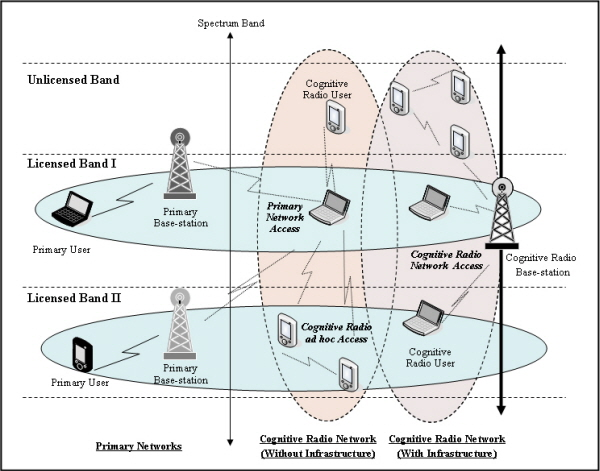
\includegraphics[width=0.5\textwidth]{myFigures/cogArch.jpg}
        \caption{Cognitive radio networks architecture~\cite{bwnGatechProjectDescription}}
        \label{fig:cogArch}
    \end{center}
\end{figure}

% Why is it interesting and important?
%The importance of our study lies on the fact that almost all the modern mobile devices contain multiple radios.

On the other hand, classical wireless networks frequently adopt the notion of deploying users with multiple radios~\cite{bahl2004reconsidering, adya2004multi}. Such deployment of multiple radios improves capacity of the networks \cite{draves2004routing, bahl2004reconsidering}, enhances loss resilience \cite{miu2005improving}, and enables heterogeneous wireless access for smart devices \cite{song2012performance}. However, this augmentation also demands modified routing, medium-access, and link-layer protocols \cite{kyasanur2006routing, chatterjee2013low}. Nonetheless, as such deployment of multiple radios in wireless nodes is known to improve the performance of a user and  deployment of cognitive radios also aims to improve the performance of secondary users through spectrum utilization, it is intuitive that simultaneous utilization of both these techniques, i.e., Cognitive Multi-Radio Networks (CMRNs), will result in significantly improved network performance. Therefore, the notion of exploiting multiple radios in CRNs to supplement the dynamic spectrum access has been proposed in the contemporary literature. Existing studies in this regard present that such multi-radio deployment in CRNs improves delay up to a certain point, however, throughput always degrades with an increase in the number of radios per secondary user~\cite{khan2015towards}. Therefore, the main motivation behind this study is to examine how to improve network throughput while equipping secondary users with multiple radios.

% Why is it hard? (E.g., why do naive approaches fail?)
The main challenge of improving total network throughput in CMRNs lies on the silent features of the architecture of CRNs. In CRNs, nodes generally have limited spectrum knowledge covering only its own neighborhood. Thus, the knowledge is conventionally gathered in a distributed manner. Therefore, graph-based and MILP optimization-based solutions~\cite{hoang2008downlink,ahmed2014channel} for improving throughput can not be directly incorporated due to their nature of performing centralized computations. Moreover, the relation between two different performance metrics (throughput and delay) may be opposing in nature~\cite{gamal2004throughput} and improving one of them may result in degradation of the another. Consequently, a trade-off between these two metrics demands special attention in CMRNs in road to improving throughput.

% Why hasn't it been solved before? (Or, what's wrong with previous proposed solutions? How does mine differ?)
Most of the existing studies on CMRNs fail to solve our research problem, as they overlook the effect of utilizing multiple radios on different performance metrics. The studies~\cite{de2012survey, feng2009joint, zhong2014capacity, li2014deterministic} usually integrate MAC and routing protocols for the multi-radio network architectures and solve the channel assignment problem for multi-channel scenario. While assigning multiple channels among multiple radios, the existing studies either randomly select the channels~\cite{khan2015towards} or only rank the channels~\cite{zhong2014capacity}. Due to all these reasons, to the best of our knowledge, no existing research study provides a viable solution for enhancing throughput in CMRNs.

% What are the key components of my approach and results? Also include any specific limitations.
To this end, in this paper, we propose to integrate feedback obtained from lower layers (Physical layer and Data Link layer) in the process of decision making in an upper layer (Application layer) to enhance network throughput. Here, to obtain lower layer feedback, we keep different packet counters for radios as well as channels in each secondary user. Using values of these counters, we rank all available radios and channels of a secondary user. Subsequently, based on the ranking, we make packet queuing decisions from the Application layer and channel switching decisions from the Data link layer while retaining a stochastic flavor. We implement our proposed feedback-based approach in \texttt{ns-3} to evaluate its performance in terms of throughput along with delay and drop ratio. Our simulation results demonstrate that the proposed approach can achieve significant improvement in terms of all the performance metrics in most of the cases.

% Summary of Contributions
%Then have a final paragraph or subsection: "Summary of Contributions". It should list the major contributions in bullet form, mentioning in which sections they can be found. This material doubles as an outline of the rest of the paper, saving space and eliminating redundancy.

%\section{Summary of Contributions}

Based on our study in this paper, we make the following set of contributions:

\begin{itemize}
\item We propose a feedback-based multi-radio exploitation approach, along with several variants, to solve the throughput degradation problem in CMRNs.
\item We implement the proposed approach and its variants in \texttt{ns-3} to demonstate their radio selection and channel selection policies.
\item We compare performance of our proposed approach against that of existing approaches in the literature. Comparative results confirm significant improvement over existing approaches through using our proposed approach.
\end{itemize}
\endinput


\chapter{Background and Related Work}\label{relatedWork}

%CRN backgrounds, motivation
Traditional analog model for spectrum management resulted into the inefficient utilization of most radio frequency spectrum~\cite{valenta2010survey}. While several mobile network spectrum bands are highly congested, other spectrum bands like TV space and non-commercial radio bands are overly under-utilized. Moreover, these utilization varies depending on time and place resulting into spectrum hole~\cite{tandra2009spectrum}. Subsequently, the notion of cognitive radio was proposed to exploit these temporal and spatial spectrum holes.

%CR definition
\section{Cognitive Radio}
Cognitive radio is a special kind of radio with two unique attributes, cognitive capability and reconfigurability~\cite{akyildiz2006next, thomas2005cognitive, haykin2005cognitive}. Cognitive capability enables cognitive radio to sense its radio environment. The radio environment sensing process involves observing the power in various spectrum bands as well as identifying temporal and spatial spectrum holes~\cite{akyildiz2006next}. On the other hand, reconfigurability helps cognitive radio to communicate over various spectrum bands to improve spectrum utilization based on its spectrum awareness~\cite{jondral2005software}.

Based on these two special characteristics, the primary objective of cognitive radio can be best understood from its widely adopted definition~\cite{federal2005notice}:

\begin{quote}
A cognitive radio is a radio or system that senses its operational electromagnetic environment and can dynamically and autonomously adjust its radio operating parameters to modify system operation, such as maximize throughput, mitigate interference, facilitate interoperability, access secondary markets.
\end{quote}

Given the fixed nature of traditional spectrum allocation, the primary challenge of cognitive radio is to exploit spectrum holes in the licensed band while not causing any interruption to the licensed users. Therefore, while using a temporally and/or spatially free spectrum, if the licensed user starts using the corresponding spectrum, the cognitive radio must have the capability to switch to another spectrum or change its other transmission parameters to avoid interruption with the licensed user. Next, we will see how does a cognitive radio achieve this in greater detail.

\subsection{Working Method of A Cognitive Radio}

\begin{figure}[!htbp]
\begin{center}
    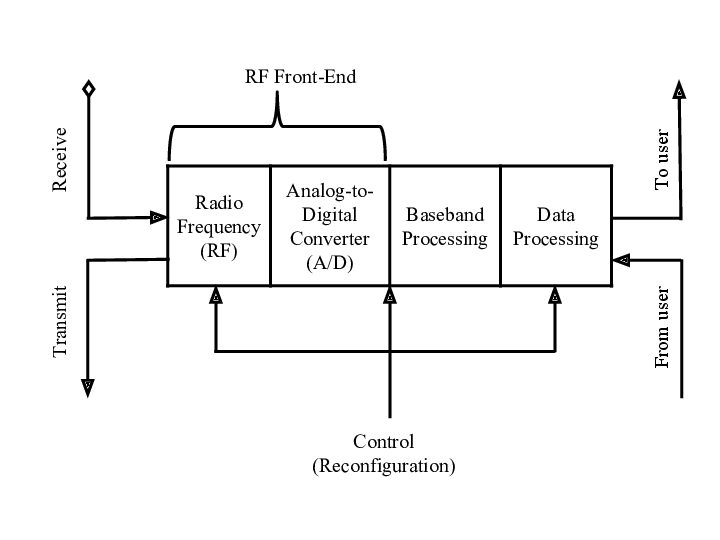
\includegraphics[scale=0.5]{myFigures/PhysicalCR}
    \caption{Cognitive radio transceiver (redrawn from~\cite{jondral2005software})}
    \label{fig:PhysicalCR}
\end{center}
\end{figure}

As shown in Figure~\ref{fig:PhysicalCR}~\cite{jondral2005software}, the cognitive radio transceiver is consisted of a radio front-end and a processing unit~\cite{akyildiz2006next}. The most important fact that distinguishes cognitive radios from other traditional radios is cognitive radio's ability to reconfigure itself via a control bus parameterizing both the radio front-end and processing units~\cite{jondral2005software}. The radio front-end amplifies and mixes the received signal and then converts it from analog to digital signal. The processing unit doing the job of baseband and data processing is quite similar to conventional radio transceivers. Nonetheless, the unique design of cognitive radio's front end also attributes to its novelty, and therefore, we will discuss the radio front-end up next.

\begin{figure}[!htbp]
\begin{center}
    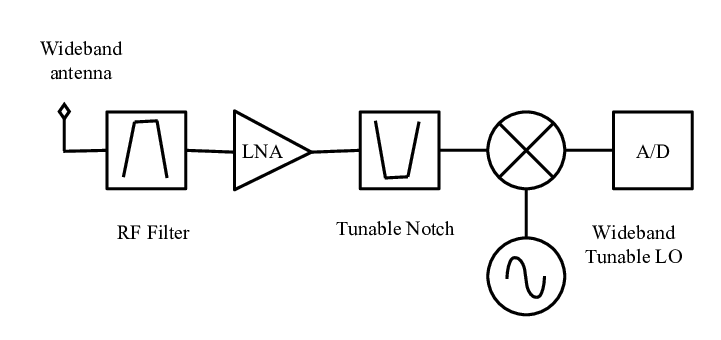
\includegraphics[scale=0.5]{myFigures/RFFrontEnd}
    \caption{Wideband RF/analog front-end architecture for cognitive radio (redrawn from~\cite{cabric2004implementation})}
    \label{fig:RFFrontEnd}
\end{center}
\end{figure}

The radio front-end of a cognitive radio is illustrated in Figure~\ref{fig:RFFrontEnd}~\cite{cabric2004implementation}. It has a wideband sensing capability mainly due to its components like wideband antenna, power amplifier, and adaptive filter. This wideband sensing capability of the radio front end enables cognitive radio to tune to any part of a wide spectrum band. This capability also helps cognitive radio to measure any spectrum information of radio surroundings. To accomplish all this, a wideband radio front-end needs to have several components~\cite{akyildiz2006next}: RF filter, low noise amplifier (LNA), tunable notch, wideband tunable local oscillator (LO), and analog to digital (A/D) converter. RF filter works as a bandpass filter selecting only the desired band RF signal. LNA minimizes the signal noise and amplifies the desired signals amplitude. Tunable notch filters the selected channel from the signal and rejects adjacent channels. Wideband tunable LO has mainly two components: voltage-controlled oscillator (VCO) and mixer. VCO usually can generate signals at any specific frequency and this locally generated RF signal is mixed with desired signal at mixer to convert it into a baseband signal. A/D converter samples and quantizes this signal with very high resolution.

Now that we have described the definition and the working procedure of cognitive radios, we will see how the cognitive radio networks (CRNs) architecture employs cognitive radios to increase spectrum utilization. 

\section{Cognitive Radio Networks (CRNs)}

The Cognitive Radio Networks (CRNs) architecture is shown in Figure~\ref{fig:cogArch}. The components of the architecture can be widely categorized in two groups, the primary network and the secondary network~\cite{akyildiz2006next}. The primary network is the existing network infrastructure. In the existing infrastructure, some spectrum bands are licensed (Example, cellular network, TV broadcast networks) and some other bands are unlicensed. Licensed band users have exclusive right to their spectrum band and are called primary users (PUs). Primary users' access to their licensed band is supervised by the primary base stations and these users require no adaptation to include in cognitive radio networks architecture. 

\begin{figure}[!htbp]
    \begin{center}
        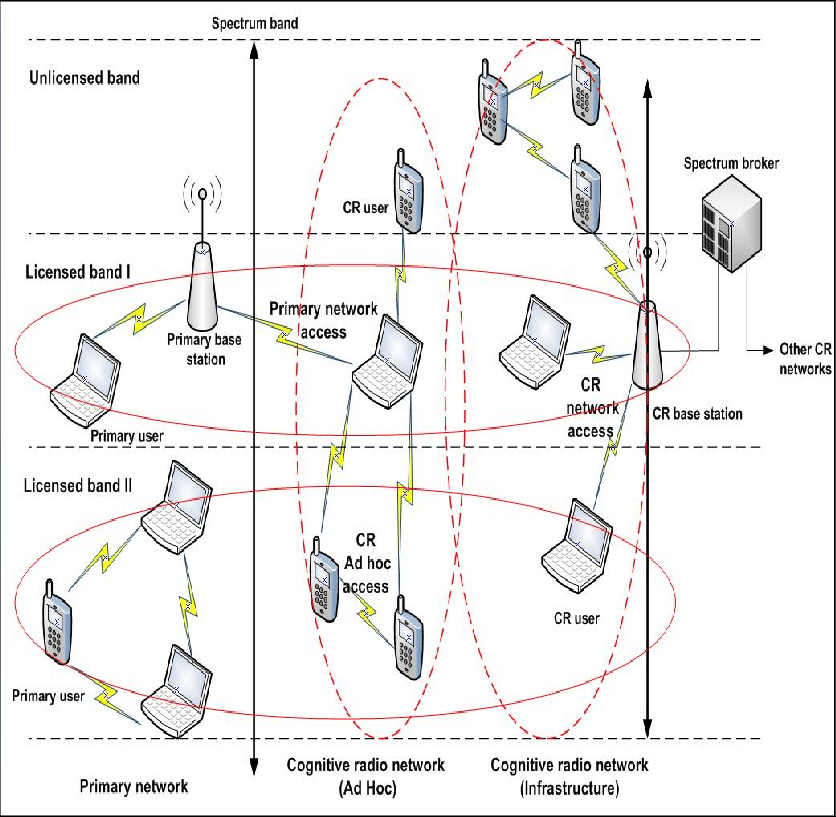
\includegraphics[width=0.6\textwidth]{myFigures/cogArch.png}
        \caption{Cognitive radio networks architecture~\cite{bwnGatechProjectDescription}}
        \label{fig:cogArch}
    \end{center}
\end{figure}

The secondary network is also known as dynamic spectrum access network, unlicensed network, xG network, and cognitive radio network~\cite{akyildiz2006next}. The users of this network contains no license to use the spectrum band and are called secondary users (SUs). These users employ cognitive radios to opportunistically exploit temporal spectrum holes. The secondary network can operate under the provision of secondary base stations or just work in an ad hoc manner. Another important component of cognitive radio networks is a central network entity called spectrum broker that works as a spectrum information manager to maintain the coexistence of multiple cognitive radio networks~\cite{akyildiz2006next, buddhikot2005dimsumnet, ileri2005demand, zekavat2005user}.

\section{Applications of CRNs}
The unconventional architecture of cognitive radio networks has several applications including high-speed rural internet infrastructure development~\cite{fitch2011wireless}, military networks~\cite{murty2003software}, emergency networks~\cite{maldonado2005cognitive}, leased networks~\cite{stine2005spectrum}, and cognitive mesh networks~\cite{berlemann2005policy}.

California based Carlson wireless technologies markets cognitive radio enabled RuralConnect device~\cite{ruralConnect}. This device exploits TV white space to deliver high speed internet connectivity to rural people. It can also be deployed in densly populated areas with significant spectrum contention.

Military networks is another significant applications of CRNs. CRNs support military radios' requirements of choosing any random frequency, modulation and coding techniques, and adaptation to the changing battle-field environment~\cite{akyildiz2006next}.

Emergency networks in the times of natural disasters can be established using CRNs. CRNs establishes such emergency networks by enabling data communication over existing spectrum without installing any new infrastructures~\cite{maldonado2005cognitive}.

\begin{figure}[!htbp]
    \begin{center}
        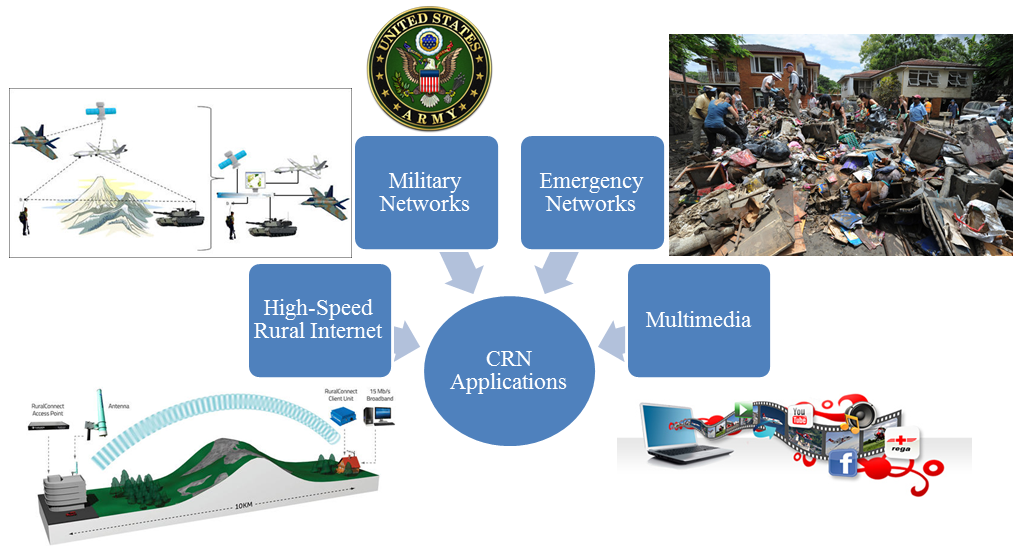
\includegraphics[width=0.8\textwidth]{myFigures/CRNApplications.png}
        \caption{Applications of cognitive radio networks~\cite{akyildiz2006next}}
        \label{fig:CRNApplications}
    \end{center}
\end{figure}

\section{Multi-Radio Networks}

The price of RF transceivers has rapidly reduced in the last few years. This price reduction has prompted to install multiple low-cost radios in a single node of wireless networks~\cite{raniwala2005architecture}. Such networks are known as multi-radio networks. These multi-radio networks impose unique research challenges due to the nature of two conflicting objectives: channel diversity and node connectivity~\cite{wang2007survey}. Multiple radios on a single node enables simultaneous multiple channel access which results in improved network capacity. On the contrary, the transmitter and the receiver must be adjusted to the same channel to maintain network connectivity. Consequently, common control radio based protocols has been proposed in the recent literature to address these challenges~\cite{ko2007distributed, al2016channel, gabale2013classification, kyasanur2006routing, chatterjee2013low}.

One of significant advantage of installing multiple radios on a single node in multi-radio networks is the network performance improvement through parallel spectrum access. On the other hand, the basic motivation behind using cognitive radio networks is also to improve network performance through opportunistic dynamic spectrum access. Therefore, these two paradigms are combined into another network architecture, multi-radio cognitive radio networks. 

\section{Multi-Radio Cognitive Radio Networks(MRCRNs)}
In multi-radio cognitive radio networks, secondary users are equipped with multiple transceivers. This enables secondary users to increase spectrum access just like any multi-radio networks. Moreover, the channel switching time for cognitive radio networks is also reduced as illustrated in Figure~\ref{fig:switchingDelay}. Secondary users have to vacant their currently used channel when the channel's licensed primary user becomes active. This results into secondary users looking for another free channel and switching into that free channel. Secondary users equipped with multiple radios can exploit their additional radios to reduce this switching delay.

\begin{figure}[!htbp]
\begin{center}
    \noindent\begin{minipage}{\textwidth}
    \begin{minipage}[c][6cm][c]{\dimexpr0.5\textwidth-0.5\Colsep\relax}
    \begin{center}
    \begin{tikzpicture} [scale=1.0, transform shape]%show background rectangle,
        \tikzstyle{every node} = [draw, shape = rectangle, node distance=0mm, minimum width=5mm, minimum height=5.2mm]
        \node[draw=black, thick, label=below:Channel 2] (channel2) {
            \begin{tikzpicture}
                \node (puidle) [fill=red!20, minimum width=30mm] {\small Busy};%
            \end{tikzpicture}
        };
        \node[draw=black, thick, label=below:Channel 1] (channel1) [above=of channel2, yshift=7.5mm] {
            \begin{tikzpicture}
                \node (pubusy) [minimum width=30mm] {\small Idle};
            \end{tikzpicture}
        };
        \node[draw=black, thick, label=below:Channel 3] (channel3) [below=of channel2, yshift=-7.5mm] {
            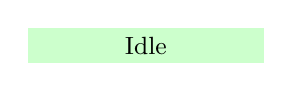
\begin{tikzpicture}
                \node (pubusy) [fill=green!20, minimum width=30mm] {\small Idle};
            \end{tikzpicture}
        };
        \node[draw=black, thick, label=below:Channel 4] (channel4) [below=of channel3, yshift=-7.5mm] {
            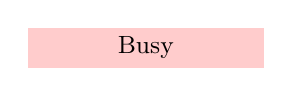
\begin{tikzpicture}
                \node (pubusy) [fill=red!20, minimum width=30mm] {\small Busy};
            \end{tikzpicture}
        };

        \node[draw] (mrcrn) [right=of channel3, yshift=0.8cm, xshift=0.25cm] {
            \begin{tikzpicture} [scale=0.625, transform shape]
            \node[draw=white, thick] (su2) [right=of channel3, xshift=1mm] {
            \begin{tikzpicture} [scale=0.5]
            \draw [line width=0.25mm, green!50!black] (2, -0.44) to (2.5,0.44);
            \draw [line width=0.25mm, green!50!black] (3, -0.44) to (2.5,0.44);
            \draw [line width=0.25mm, green!50!black] (2, -0.44) to (3,-0.44);
            \draw [line width=0.25mm, green!50!black] (2.5, -0.44) to (2.5,0.44);
            \draw [fill=green!50!black, green!50!black] (2.5,0.44) circle(1.5mm);

            \draw [line width=0.25mm, green!50!black] (2.5, 0.725) to (2.5,1.0);
            \draw [line width=0.25mm, green!50!black] (2.65, 0.65) to (2.825,0.85);
            \draw [line width=0.25mm, green!50!black] (2.725, 0.44) to (3,0.44);
            \draw [line width=0.25mm, green!50!black] (2.35, 0.65) to (2.175,0.85);
            \draw [line width=0.25mm, green!50!black] (2.275, 0.44) to (2,0.44);

            \end{tikzpicture}
        };

        

        \node[draw=white, thick] (su3) [right=of channel2, xshift=1mm] {
            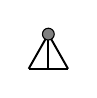
\begin{tikzpicture} [scale=0.5]
            \draw [line width=0.25mm] (2, -0.44) to (2.5,0.44);
            \draw [line width=0.25mm] (3, -0.44) to (2.5,0.44);
            \draw [line width=0.25mm] (2, -0.44) to (3,-0.44);
            \draw [line width=0.25mm] (2.5, -0.44) to (2.5,0.44);
            \draw [fill=gray] (2.5,0.44) circle(1.5mm);

            \end{tikzpicture}
        };
        
        \end{tikzpicture}
        };

        \node[draw=white, thick] (pu1) [left=of channel1, xshift=-1mm] {
            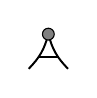
\begin{tikzpicture} [scale=0.5]
            \draw [line width=0.25mm, bend right = 15] (2, -0.44) to (2.5,0.44);
            \draw [line width=0.25mm, bend left = 15] (3, -0.44) to (2.5,0.44);
            \draw [line width=0.25mm] (2.25, -0.15) to (2.75,-0.15);
            %\draw [line width=0.25mm] (2.5, -0.44) to (2.5,0.44);
            \draw [fill=gray] (2.5,0.44) circle(1.5mm);

            \end{tikzpicture}
        };

        \node[draw=white, thick] (pu2) [left=of channel2, xshift=-1mm] {
            
\begin{tikzpicture} [scale=0.5]
            \draw [line width=0.25mm, bend right = 15, red] (2, -0.44) to (2.5,0.44);
            \draw [line width=0.25mm, bend left = 15, red] (3, -0.44) to (2.5,0.44);
            \draw [line width=0.25mm, red] (2.25, -0.15) to (2.75,-0.15);
            %\draw [line width=0.25mm] (2.5, -0.44) to (2.5,0.44);
            \draw [fill=red, red] (2.5,0.44) circle(1.5mm);

            \draw [line width=0.25mm, red] (2.5, 0.725) to (2.5,1.0);
            \draw [line width=0.25mm, red] (2.65, 0.65) to (2.825,0.85);
            \draw [line width=0.25mm, red] (2.725, 0.44) to (3,0.44);
            \draw [line width=0.25mm, red] (2.35, 0.65) to (2.175,0.85);
            \draw [line width=0.25mm, red] (2.275, 0.44) to (2,0.44);

            \end{tikzpicture}
        };

        \node[draw=white, thick] (pu3) [left=of channel3, xshift=-1mm] {
            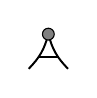
\begin{tikzpicture} [scale=0.5]
            \draw [line width=0.25mm, bend right = 15] (2, -0.44) to (2.5,0.44);
            \draw [line width=0.25mm, bend left = 15] (3, -0.44) to (2.5,0.44);
            \draw [line width=0.25mm] (2.25, -0.15) to (2.75,-0.15);
            %\draw [line width=0.25mm] (2.5, -0.44) to (2.5,0.44);
            \draw [fill=gray] (2.5,0.44) circle(1.5mm);

            \end{tikzpicture}
        };

        \node[draw=white, thick] (pu4) [left=of channel4, xshift=-1mm] {
            
\begin{tikzpicture} [scale=0.5]
            \draw [line width=0.25mm, bend right = 15, red] (2, -0.44) to (2.5,0.44);
            \draw [line width=0.25mm, bend left = 15, red] (3, -0.44) to (2.5,0.44);
            \draw [line width=0.25mm, red] (2.25, -0.15) to (2.75,-0.15);
            %\draw [line width=0.25mm] (2.5, -0.44) to (2.5,0.44);
            \draw [fill=red, red] (2.5,0.44) circle(1.5mm);

            \draw [line width=0.25mm, red] (2.5, 0.725) to (2.5,1.0);
            \draw [line width=0.25mm, red] (2.65, 0.65) to (2.825,0.85);
            \draw [line width=0.25mm, red] (2.725, 0.44) to (3,0.44);
            \draw [line width=0.25mm, red] (2.35, 0.65) to (2.175,0.85);
            \draw [line width=0.25mm, red] (2.275, 0.44) to (2,0.44);

            \end{tikzpicture}
        };
    \end{tikzpicture}
    \end{center}
    \end{minipage}\hfill
    \begin{minipage}[c][6cm][c]{\dimexpr0.5\textwidth-0.5\Colsep\relax}
    \begin{center}
    \begin{tikzpicture} [scale=1.0, transform shape]%show background rectangle,
        \tikzstyle{every node} = [draw, shape = rectangle, node distance=0mm, minimum width=5mm, minimum height=5.2mm]
        \node[draw=black, thick, label=below:Channel 2] (channel2) {
            \begin{tikzpicture}
                \node (puidle) [fill=green!20, minimum width=30mm] {\small Idle};%
            \end{tikzpicture}
        };
        \node[draw=black, thick, label=below:Channel 1] (channel1) [above=of channel2, yshift=7.5mm] {
            \begin{tikzpicture}
                \node (pubusy) [minimum width=30mm] {\small Idle};
            \end{tikzpicture}
        };
        \node[draw=black, thick, label=below:Channel 3] (channel3) [below=of channel2, yshift=-7.5mm] {
            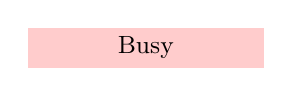
\begin{tikzpicture}
                \node (pubusy) [fill=red!20, minimum width=30mm] {\small Busy};
            \end{tikzpicture}
        };
        \node[draw=black, thick, label=below:Channel 4] (channel4) [below=of channel3, yshift=-7.5mm] {
            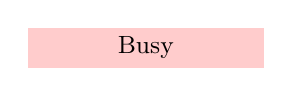
\begin{tikzpicture}
                \node (pubusy) [fill=red!20, minimum width=30mm] {\small Busy};
            \end{tikzpicture}
        };

        \node[draw] (mrcrn) [right=of channel3, yshift=0.8cm, xshift=0.25cm] {
            \begin{tikzpicture} [scale=0.625, transform shape]

        

        \node[draw=white, thick] (su2) [right=of channel3, xshift=1mm] {
            \begin{tikzpicture} [scale=0.5]
            \draw [line width=0.25mm] (2, -0.44) to (2.5,0.44);
            \draw [line width=0.25mm] (3, -0.44) to (2.5,0.44);
            \draw [line width=0.25mm] (2, -0.44) to (3,-0.44);
            \draw [line width=0.25mm] (2.5, -0.44) to (2.5,0.44);
            \draw [fill=gray] (2.5,0.44) circle(1.5mm);

            \end{tikzpicture}
        };

        \node[draw=white, thick] (su3) [right=of channel2, xshift=1mm] {
            
\begin{tikzpicture} [scale=0.5]
            \draw [line width=0.25mm, green!50!black] (2, -0.44) to (2.5,0.44);
            \draw [line width=0.25mm, green!50!black] (3, -0.44) to (2.5,0.44);
            \draw [line width=0.25mm, green!50!black] (2, -0.44) to (3,-0.44);
            \draw [line width=0.25mm, green!50!black] (2.5, -0.44) to (2.5,0.44);
            \draw [fill=green!50!black, green!50!black] (2.5,0.44) circle(1.5mm);

            \draw [line width=0.25mm, green!50!black] (2.5, 0.725) to (2.5,1.0);
            \draw [line width=0.25mm, green!50!black] (2.65, 0.65) to (2.825,0.85);
            \draw [line width=0.25mm, green!50!black] (2.725, 0.44) to (3,0.44);
            \draw [line width=0.25mm, green!50!black] (2.35, 0.65) to (2.175,0.85);
            \draw [line width=0.25mm, green!50!black] (2.275, 0.44) to (2,0.44);

            \end{tikzpicture}
        };
        \end{tikzpicture}
        };

        \node[draw=white, thick] (pu1) [left=of channel1, xshift=-1mm] {
            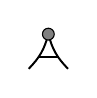
\begin{tikzpicture} [scale=0.5]
            \draw [line width=0.25mm, bend right = 15] (2, -0.44) to (2.5,0.44);
            \draw [line width=0.25mm, bend left = 15] (3, -0.44) to (2.5,0.44);
            \draw [line width=0.25mm] (2.25, -0.15) to (2.75,-0.15);
            %\draw [line width=0.25mm] (2.5, -0.44) to (2.5,0.44);
            \draw [fill=gray] (2.5,0.44) circle(1.5mm);

            \end{tikzpicture}
        };

        \node[draw=white, thick] (pu2) [left=of channel2, xshift=-1mm] {
            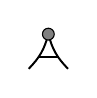
\begin{tikzpicture} [scale=0.5]
            \draw [line width=0.25mm, bend right = 15] (2, -0.44) to (2.5,0.44);
            \draw [line width=0.25mm, bend left = 15] (3, -0.44) to (2.5,0.44);
            \draw [line width=0.25mm] (2.25, -0.15) to (2.75,-0.15);
            %\draw [line width=0.25mm] (2.5, -0.44) to (2.5,0.44);
            \draw [fill=gray] (2.5,0.44) circle(1.5mm);

            \end{tikzpicture}
        };

        \node[draw=white, thick] (pu3) [left=of channel3, xshift=-1mm] {
            
\begin{tikzpicture} [scale=0.5]
            \draw [line width=0.25mm, bend right = 15, red] (2, -0.44) to (2.5,0.44);
            \draw [line width=0.25mm, bend left = 15, red] (3, -0.44) to (2.5,0.44);
            \draw [line width=0.25mm, red] (2.25, -0.15) to (2.75,-0.15);
            %\draw [line width=0.25mm] (2.5, -0.44) to (2.5,0.44);
            \draw [fill=red, red] (2.5,0.44) circle(1.5mm);

            \draw [line width=0.25mm, red] (2.5, 0.725) to (2.5,1.0);
            \draw [line width=0.25mm, red] (2.65, 0.65) to (2.825,0.85);
            \draw [line width=0.25mm, red] (2.725, 0.44) to (3,0.44);
            \draw [line width=0.25mm, red] (2.35, 0.65) to (2.175,0.85);
            \draw [line width=0.25mm, red] (2.275, 0.44) to (2,0.44);

            \end{tikzpicture}
        };

        \node[draw=white, thick] (pu4) [left=of channel4, xshift=-1mm] {
            
\begin{tikzpicture} [scale=0.5]
            \draw [line width=0.25mm, bend right = 15, red] (2, -0.44) to (2.5,0.44);
            \draw [line width=0.25mm, bend left = 15, red] (3, -0.44) to (2.5,0.44);
            \draw [line width=0.25mm, red] (2.25, -0.15) to (2.75,-0.15);
            %\draw [line width=0.25mm] (2.5, -0.44) to (2.5,0.44);
            \draw [fill=red, red] (2.5,0.44) circle(1.5mm);

            \draw [line width=0.25mm, red] (2.5, 0.725) to (2.5,1.0);
            \draw [line width=0.25mm, red] (2.65, 0.65) to (2.825,0.85);
            \draw [line width=0.25mm, red] (2.725, 0.44) to (3,0.44);
            \draw [line width=0.25mm, red] (2.35, 0.65) to (2.175,0.85);
            \draw [line width=0.25mm, red] (2.275, 0.44) to (2,0.44);

            \end{tikzpicture}
        };
    \end{tikzpicture}
    \end{center}
    \end{minipage}%
\end{minipage}

    \caption{Secondary users (SUs) equipped with multiple radios experience reduced switching delay}
    \label{fig:switchingDelay}
\end{center}
\end{figure}

Due to these advantages, several studies have investigated the various research problems in MRCRNs. In next section, we will survey the existing research works on MRCRNs.

\section{Existing Studies on MRCRNs}
Existing studies on MRCRNs mainly investigate how to incorporate multiple radios in dynamic spectrum sharing scenario. These studies mainly propose medium access control protocols~\cite{cormio2009survey, de2012survey}, routing protocols~\cite{zhu2008stod, feng2009joint}, and channel assignment~\cite{ahmadi2012distributed, zhong2014capacity} for MRCRNs. Zhu et al., present a spectrum-tree based on-demand routing protocol that considers multi-radio nodes~\cite{zhu2008stod}. Such nodes belong to multiple spectrum-trees and are called overlapping nodes. As these nodes simultaneously work in different spectrum-trees, they can be used for inter-spectrum routing. The study shows that the proposed approach significantly reduces the average end-to-end delay.  Besides, Feng et al., propose a novel spectrum handoff scheduling approach for multi-hop MRCRNs~\cite{feng2009joint}. This study presents a routing protocol with the help of aging-based priority assignment to minimize the latency. Thus none of these approaches addresses the problem of overcoming throughput degradation problem in MRCRNs.

Ahmadi et al., present one of the earliest CRN studies involving multiple radios, which considers two sender radios for each secondary user~\cite{ahmadi2012distributed}. This study strives to solve channel assignment problem for the scenario. However, as there is only one receiver radio for each user in the proposed network model and channels are assigned to the receiver radio, the corresponding channel assignment problem becomes close to the single-radio channel assignment problem. This is because, as in single-radio scenario, only one channel needs to be assigned for each receiver node and the node can not exploit multiple available channels while receiving packets. Further, the study always uses a fixed number of transmitter radios (two) and do not investigate performance of the network for varying numbers of radios.

Another MRCRN study~\cite{zhong2014capacity} by Zhong et al., aims to solve the channel assignment problem for MRCRNs. Here, their proposed channel assignment approach assigns multiple channels among multiple radios available for secondary users. Despite ranking channels, while assigning them among radios, the approach does not consider the state of those radios. Besides, the paper does not provide any analysis on throughput with an increase in the number of radios.

The analysis of any performance metric based on an increase in the number of radios in CRNs is first presented in the study~\cite{li2014deterministic} by Li et al., to the best of our knowledge. The study presents a rendezvous channel establishment approach for MRCRNs. It shows that the maximum time to rendezvous reduces with an increase in the number of radios used in CRNs. However, the study does not provide any solution on how these radios will be used for data transmission and its subsequent effect on performance metrics such as throughput and delay.

Later, Khan et al.,~\cite{khan2015towards} propose another MRCRNs architecture where each secondary user employs multiple radios for data transmission. The study shows that per packet average end-to-end delay gets improved at the cost of throughput degradation with an increase in the number of radios. This study does the radio-channel assignment in a random manner and does not avoid inter-user channel interface. Thus, this study fails to improve throughput with an increase in the number of radios.

In summary, none of the existing studies focuses on enhancing throughput in MRCRNs. Therefore, we attempt to propose a new channel assignment approach to enhance throughput in MRCRNs in this thesis. Before presenting the approach, we first elaborate our system model and problem formulation.
\endinput


\begin{tikzpicture}[scale=1.0, transform shape]
    %\draw [help lines] (0, 0) grid (10, 7);
    \draw (0, 0) node {\begin{tikzpicture}[scale=1.0, transform shape]
    \node[draw=white, thick] (puRadio) {
        \begin{tikzpicture} [scale=0.5]
        \draw [line width=0.25mm, bend right = 15, red] (2, -0.44) to (2.5,0.44);
        \draw [line width=0.25mm, bend left = 15, red] (3, -0.44) to (2.5,0.44);
        \draw [line width=0.25mm, red] (2.15, -0.3) to (2.85,-0.3);
        \draw [line width=0.25mm, red] (2.25, -0.15) to (2.75,-0.15);
        \draw [line width=0.25mm, red] (2.35, 0) to (2.65,0);
        %\draw [line width=0.25mm] (2.5, -0.44) to (2.5,0.44);
        \draw [fill=red, red] (2.5,0.44) circle(1.5mm);

        \draw [line width=0.25mm, red] (2.5, 0.725) to (2.5,1.0);
        \draw [line width=0.25mm, red] (2.65, 0.65) to (2.825,0.85);
        \draw [line width=0.25mm, red] (2.725, 0.44) to (3,0.44);
        \draw [line width=0.25mm, red] (2.35, 0.65) to (2.175,0.85);
        \draw [line width=0.25mm, red] (2.275, 0.44) to (2,0.44);

        \end{tikzpicture}
    };
\end{tikzpicture}};
    \draw (0, 7) node {\begin{tikzpicture}[scale=1.0, transform shape]
    \node[draw=white, thick] (puRadio) {
        \begin{tikzpicture} [scale=0.5]
        \draw [line width=0.25mm, bend right = 15, red] (2, -0.44) to (2.5,0.44);
        \draw [line width=0.25mm, bend left = 15, red] (3, -0.44) to (2.5,0.44);
        \draw [line width=0.25mm, red] (2.15, -0.3) to (2.85,-0.3);
        \draw [line width=0.25mm, red] (2.25, -0.15) to (2.75,-0.15);
        \draw [line width=0.25mm, red] (2.35, 0) to (2.65,0);
        %\draw [line width=0.25mm] (2.5, -0.44) to (2.5,0.44);
        \draw [fill=red, red] (2.5,0.44) circle(1.5mm);

        \draw [line width=0.25mm, red] (2.5, 0.725) to (2.5,1.0);
        \draw [line width=0.25mm, red] (2.65, 0.65) to (2.825,0.85);
        \draw [line width=0.25mm, red] (2.725, 0.44) to (3,0.44);
        \draw [line width=0.25mm, red] (2.35, 0.65) to (2.175,0.85);
        \draw [line width=0.25mm, red] (2.275, 0.44) to (2,0.44);

        \end{tikzpicture}
    };
\end{tikzpicture}};
    \draw (10, 7) node {\begin{tikzpicture}[scale=1.0, transform shape]
    \node[draw=white, thick] (puRadio) {
        \begin{tikzpicture} [scale=0.5]
        \draw [line width=0.25mm, bend right = 15, red] (2, -0.44) to (2.5,0.44);
        \draw [line width=0.25mm, bend left = 15, red] (3, -0.44) to (2.5,0.44);
        \draw [line width=0.25mm, red] (2.15, -0.3) to (2.85,-0.3);
        \draw [line width=0.25mm, red] (2.25, -0.15) to (2.75,-0.15);
        \draw [line width=0.25mm, red] (2.35, 0) to (2.65,0);
        %\draw [line width=0.25mm] (2.5, -0.44) to (2.5,0.44);
        \draw [fill=red, red] (2.5,0.44) circle(1.5mm);

        \draw [line width=0.25mm, red] (2.5, 0.725) to (2.5,1.0);
        \draw [line width=0.25mm, red] (2.65, 0.65) to (2.825,0.85);
        \draw [line width=0.25mm, red] (2.725, 0.44) to (3,0.44);
        \draw [line width=0.25mm, red] (2.35, 0.65) to (2.175,0.85);
        \draw [line width=0.25mm, red] (2.275, 0.44) to (2,0.44);

        \end{tikzpicture}
    };
\end{tikzpicture}};
    \draw (10, 0) node {\begin{tikzpicture}[scale=1.0, transform shape]
    \node[draw=white, thick] (puRadio) {
        \begin{tikzpicture} [scale=0.5]
        \draw [line width=0.25mm, bend right = 15, red] (2, -0.44) to (2.5,0.44);
        \draw [line width=0.25mm, bend left = 15, red] (3, -0.44) to (2.5,0.44);
        \draw [line width=0.25mm, red] (2.15, -0.3) to (2.85,-0.3);
        \draw [line width=0.25mm, red] (2.25, -0.15) to (2.75,-0.15);
        \draw [line width=0.25mm, red] (2.35, 0) to (2.65,0);
        %\draw [line width=0.25mm] (2.5, -0.44) to (2.5,0.44);
        \draw [fill=red, red] (2.5,0.44) circle(1.5mm);

        \draw [line width=0.25mm, red] (2.5, 0.725) to (2.5,1.0);
        \draw [line width=0.25mm, red] (2.65, 0.65) to (2.825,0.85);
        \draw [line width=0.25mm, red] (2.725, 0.44) to (3,0.44);
        \draw [line width=0.25mm, red] (2.35, 0.65) to (2.175,0.85);
        \draw [line width=0.25mm, red] (2.275, 0.44) to (2,0.44);

        \end{tikzpicture}
    };
\end{tikzpicture}};
    %\draw [fill=green!50!white] (-2, -2) rectangle (2, -1);
    
    \draw (5, 6.2) node {\begin{tikzpicture}[scale=0.375, transform shape]
    \node (controlRadio)
    {
        \begin{tikzpicture} [scale=1.0]
        \draw [fill=blue!25!white, blue!75!black] (2.3, -0.44) -- (2.5,0.44) -- (2.7, -0.44);
        \draw [fill=blue!25!white, blue!75!black] (2.5,0.44) circle(1.5mm);

        \draw [line width=0.25mm, blue!25!white] (2.5, 0.725) to (2.5,1.0);
        \draw [line width=0.25mm, blue!25!white] (2.65, 0.65) to (2.825,0.85);
        \draw [line width=0.25mm, blue!25!white] (2.725, 0.44) to (3,0.44);
        \draw [line width=0.25mm, blue!25!white] (2.35, 0.65) to (2.175,0.85);
        \draw [line width=0.25mm, blue!25!white] (2.275, 0.44) to (2,0.44);

        \end{tikzpicture}
    };
    \node (dataRadio1) [below=of controlRadio, xshift=-1.0cm, yshift=0.5cm] %, xshift=-1.5mm
    {
        
\begin{tikzpicture} [scale=0.75]
        \draw [line width=0.25mm, green!50!black] (2, -0.44) to (2.5,0.44);
        \draw [line width=0.25mm, green!50!black] (3, -0.44) to (2.5,0.44);
        \draw [line width=0.25mm, green!50!black] (2, -0.44) to (3,-0.44);
        \draw [line width=0.25mm, green!50!black] (2.5, -0.44) to (2.5,0.44);
        \draw [fill=green!50!black, green!50!black] (2.5,0.44) circle(1.5mm);

        \draw [line width=0.25mm, green!50!black] (2.5, 0.725) to (2.5,1.0);
        \draw [line width=0.25mm, green!50!black] (2.65, 0.65) to (2.825,0.85);
        \draw [line width=0.25mm, green!50!black] (2.725, 0.44) to (3,0.44);
        \draw [line width=0.25mm, green!50!black] (2.35, 0.65) to (2.175,0.85);
        \draw [line width=0.25mm, green!50!black] (2.275, 0.44) to (2,0.44);

        \end{tikzpicture}
    };
    %()
    \draw[fill=green!50!black, green!50!black] (-0.25,-2.15) circle (0.025);
    \draw[fill=green!50!black, green!50!black] (0,-2.15) circle (0.025);
    \draw[fill=green!50!black, green!50!black] (0.25,-2.15) circle (0.025);
    %
    \node (dataRadio2) [right=of dataRadio1] %, xshift=-1.5mm
    {
        
\begin{tikzpicture} [scale=0.75]
        \draw [line width=0.25mm, green!50!black] (2, -0.44) to (2.5,0.44);
        \draw [line width=0.25mm, green!50!black] (3, -0.44) to (2.5,0.44);
        \draw [line width=0.25mm, green!50!black] (2, -0.44) to (3,-0.44);
        \draw [line width=0.25mm, green!50!black] (2.5, -0.44) to (2.5,0.44);
        \draw [fill=green!50!black, green!50!black] (2.5,0.44) circle(1.5mm);

        \draw [line width=0.25mm, green!50!black] (2.5, 0.725) to (2.5,1.0);
        \draw [line width=0.25mm, green!50!black] (2.65, 0.65) to (2.825,0.85);
        \draw [line width=0.25mm, green!50!black] (2.725, 0.44) to (3,0.44);
        \draw [line width=0.25mm, green!50!black] (2.35, 0.65) to (2.175,0.85);
        \draw [line width=0.25mm, green!50!black] (2.275, 0.44) to (2,0.44);

        \end{tikzpicture}
    };%fill=green!50!black,
    \draw[line width=0.25mm, green!25!black] (0.25,-1) circle (3);
\end{tikzpicture}
};
    \draw (1.5, 4) node {\begin{tikzpicture}[scale=0.375, transform shape]
    \node (controlRadio)
    {
        \begin{tikzpicture} [scale=1.0]
        \draw [fill=blue!25!white, blue!75!black] (2.3, -0.44) -- (2.5,0.44) -- (2.7, -0.44);
        \draw [fill=blue!25!white, blue!75!black] (2.5,0.44) circle(1.5mm);

        \draw [line width=0.25mm, blue!25!white] (2.5, 0.725) to (2.5,1.0);
        \draw [line width=0.25mm, blue!25!white] (2.65, 0.65) to (2.825,0.85);
        \draw [line width=0.25mm, blue!25!white] (2.725, 0.44) to (3,0.44);
        \draw [line width=0.25mm, blue!25!white] (2.35, 0.65) to (2.175,0.85);
        \draw [line width=0.25mm, blue!25!white] (2.275, 0.44) to (2,0.44);

        \end{tikzpicture}
    };
    \node (dataRadio1) [below=of controlRadio, xshift=-1.0cm, yshift=0.5cm] %, xshift=-1.5mm
    {
        
\begin{tikzpicture} [scale=0.75]
        \draw [line width=0.25mm, green!50!black] (2, -0.44) to (2.5,0.44);
        \draw [line width=0.25mm, green!50!black] (3, -0.44) to (2.5,0.44);
        \draw [line width=0.25mm, green!50!black] (2, -0.44) to (3,-0.44);
        \draw [line width=0.25mm, green!50!black] (2.5, -0.44) to (2.5,0.44);
        \draw [fill=green!50!black, green!50!black] (2.5,0.44) circle(1.5mm);

        \draw [line width=0.25mm, green!50!black] (2.5, 0.725) to (2.5,1.0);
        \draw [line width=0.25mm, green!50!black] (2.65, 0.65) to (2.825,0.85);
        \draw [line width=0.25mm, green!50!black] (2.725, 0.44) to (3,0.44);
        \draw [line width=0.25mm, green!50!black] (2.35, 0.65) to (2.175,0.85);
        \draw [line width=0.25mm, green!50!black] (2.275, 0.44) to (2,0.44);

        \end{tikzpicture}
    };
    %()
    \draw[fill=green!50!black, green!50!black] (-0.25,-2.15) circle (0.025);
    \draw[fill=green!50!black, green!50!black] (0,-2.15) circle (0.025);
    \draw[fill=green!50!black, green!50!black] (0.25,-2.15) circle (0.025);
    %
    \node (dataRadio2) [right=of dataRadio1] %, xshift=-1.5mm
    {
        
\begin{tikzpicture} [scale=0.75]
        \draw [line width=0.25mm, green!50!black] (2, -0.44) to (2.5,0.44);
        \draw [line width=0.25mm, green!50!black] (3, -0.44) to (2.5,0.44);
        \draw [line width=0.25mm, green!50!black] (2, -0.44) to (3,-0.44);
        \draw [line width=0.25mm, green!50!black] (2.5, -0.44) to (2.5,0.44);
        \draw [fill=green!50!black, green!50!black] (2.5,0.44) circle(1.5mm);

        \draw [line width=0.25mm, green!50!black] (2.5, 0.725) to (2.5,1.0);
        \draw [line width=0.25mm, green!50!black] (2.65, 0.65) to (2.825,0.85);
        \draw [line width=0.25mm, green!50!black] (2.725, 0.44) to (3,0.44);
        \draw [line width=0.25mm, green!50!black] (2.35, 0.65) to (2.175,0.85);
        \draw [line width=0.25mm, green!50!black] (2.275, 0.44) to (2,0.44);

        \end{tikzpicture}
    };%fill=green!50!black,
    \draw[line width=0.25mm, green!25!black] (0.25,-1) circle (3);
\end{tikzpicture}
};
    \draw (2.5, 1) node {\begin{tikzpicture}[scale=0.375, transform shape]
    \node (controlRadio)
    {
        \begin{tikzpicture} [scale=1.0]
        \draw [fill=blue!25!white, blue!75!black] (2.3, -0.44) -- (2.5,0.44) -- (2.7, -0.44);
        \draw [fill=blue!25!white, blue!75!black] (2.5,0.44) circle(1.5mm);

        \draw [line width=0.25mm, blue!25!white] (2.5, 0.725) to (2.5,1.0);
        \draw [line width=0.25mm, blue!25!white] (2.65, 0.65) to (2.825,0.85);
        \draw [line width=0.25mm, blue!25!white] (2.725, 0.44) to (3,0.44);
        \draw [line width=0.25mm, blue!25!white] (2.35, 0.65) to (2.175,0.85);
        \draw [line width=0.25mm, blue!25!white] (2.275, 0.44) to (2,0.44);

        \end{tikzpicture}
    };
    \node (dataRadio1) [below=of controlRadio, xshift=-1.0cm, yshift=0.5cm] %, xshift=-1.5mm
    {
        
\begin{tikzpicture} [scale=0.75]
        \draw [line width=0.25mm, green!50!black] (2, -0.44) to (2.5,0.44);
        \draw [line width=0.25mm, green!50!black] (3, -0.44) to (2.5,0.44);
        \draw [line width=0.25mm, green!50!black] (2, -0.44) to (3,-0.44);
        \draw [line width=0.25mm, green!50!black] (2.5, -0.44) to (2.5,0.44);
        \draw [fill=green!50!black, green!50!black] (2.5,0.44) circle(1.5mm);

        \draw [line width=0.25mm, green!50!black] (2.5, 0.725) to (2.5,1.0);
        \draw [line width=0.25mm, green!50!black] (2.65, 0.65) to (2.825,0.85);
        \draw [line width=0.25mm, green!50!black] (2.725, 0.44) to (3,0.44);
        \draw [line width=0.25mm, green!50!black] (2.35, 0.65) to (2.175,0.85);
        \draw [line width=0.25mm, green!50!black] (2.275, 0.44) to (2,0.44);

        \end{tikzpicture}
    };
    %()
    \draw[fill=green!50!black, green!50!black] (-0.25,-2.15) circle (0.025);
    \draw[fill=green!50!black, green!50!black] (0,-2.15) circle (0.025);
    \draw[fill=green!50!black, green!50!black] (0.25,-2.15) circle (0.025);
    %
    \node (dataRadio2) [right=of dataRadio1] %, xshift=-1.5mm
    {
        
\begin{tikzpicture} [scale=0.75]
        \draw [line width=0.25mm, green!50!black] (2, -0.44) to (2.5,0.44);
        \draw [line width=0.25mm, green!50!black] (3, -0.44) to (2.5,0.44);
        \draw [line width=0.25mm, green!50!black] (2, -0.44) to (3,-0.44);
        \draw [line width=0.25mm, green!50!black] (2.5, -0.44) to (2.5,0.44);
        \draw [fill=green!50!black, green!50!black] (2.5,0.44) circle(1.5mm);

        \draw [line width=0.25mm, green!50!black] (2.5, 0.725) to (2.5,1.0);
        \draw [line width=0.25mm, green!50!black] (2.65, 0.65) to (2.825,0.85);
        \draw [line width=0.25mm, green!50!black] (2.725, 0.44) to (3,0.44);
        \draw [line width=0.25mm, green!50!black] (2.35, 0.65) to (2.175,0.85);
        \draw [line width=0.25mm, green!50!black] (2.275, 0.44) to (2,0.44);

        \end{tikzpicture}
    };%fill=green!50!black,
    \draw[line width=0.25mm, green!25!black] (0.25,-1) circle (3);
\end{tikzpicture}
};
    \draw (7.5, 1) node {\begin{tikzpicture}[scale=0.375, transform shape]
    \node (controlRadio)
    {
        \begin{tikzpicture} [scale=1.0]
        \draw [fill=blue!25!white, blue!75!black] (2.3, -0.44) -- (2.5,0.44) -- (2.7, -0.44);
        \draw [fill=blue!25!white, blue!75!black] (2.5,0.44) circle(1.5mm);

        \draw [line width=0.25mm, blue!25!white] (2.5, 0.725) to (2.5,1.0);
        \draw [line width=0.25mm, blue!25!white] (2.65, 0.65) to (2.825,0.85);
        \draw [line width=0.25mm, blue!25!white] (2.725, 0.44) to (3,0.44);
        \draw [line width=0.25mm, blue!25!white] (2.35, 0.65) to (2.175,0.85);
        \draw [line width=0.25mm, blue!25!white] (2.275, 0.44) to (2,0.44);

        \end{tikzpicture}
    };
    \node (dataRadio1) [below=of controlRadio, xshift=-1.0cm, yshift=0.5cm] %, xshift=-1.5mm
    {
        
\begin{tikzpicture} [scale=0.75]
        \draw [line width=0.25mm, green!50!black] (2, -0.44) to (2.5,0.44);
        \draw [line width=0.25mm, green!50!black] (3, -0.44) to (2.5,0.44);
        \draw [line width=0.25mm, green!50!black] (2, -0.44) to (3,-0.44);
        \draw [line width=0.25mm, green!50!black] (2.5, -0.44) to (2.5,0.44);
        \draw [fill=green!50!black, green!50!black] (2.5,0.44) circle(1.5mm);

        \draw [line width=0.25mm, green!50!black] (2.5, 0.725) to (2.5,1.0);
        \draw [line width=0.25mm, green!50!black] (2.65, 0.65) to (2.825,0.85);
        \draw [line width=0.25mm, green!50!black] (2.725, 0.44) to (3,0.44);
        \draw [line width=0.25mm, green!50!black] (2.35, 0.65) to (2.175,0.85);
        \draw [line width=0.25mm, green!50!black] (2.275, 0.44) to (2,0.44);

        \end{tikzpicture}
    };
    %()
    \draw[fill=green!50!black, green!50!black] (-0.25,-2.15) circle (0.025);
    \draw[fill=green!50!black, green!50!black] (0,-2.15) circle (0.025);
    \draw[fill=green!50!black, green!50!black] (0.25,-2.15) circle (0.025);
    %
    \node (dataRadio2) [right=of dataRadio1] %, xshift=-1.5mm
    {
        
\begin{tikzpicture} [scale=0.75]
        \draw [line width=0.25mm, green!50!black] (2, -0.44) to (2.5,0.44);
        \draw [line width=0.25mm, green!50!black] (3, -0.44) to (2.5,0.44);
        \draw [line width=0.25mm, green!50!black] (2, -0.44) to (3,-0.44);
        \draw [line width=0.25mm, green!50!black] (2.5, -0.44) to (2.5,0.44);
        \draw [fill=green!50!black, green!50!black] (2.5,0.44) circle(1.5mm);

        \draw [line width=0.25mm, green!50!black] (2.5, 0.725) to (2.5,1.0);
        \draw [line width=0.25mm, green!50!black] (2.65, 0.65) to (2.825,0.85);
        \draw [line width=0.25mm, green!50!black] (2.725, 0.44) to (3,0.44);
        \draw [line width=0.25mm, green!50!black] (2.35, 0.65) to (2.175,0.85);
        \draw [line width=0.25mm, green!50!black] (2.275, 0.44) to (2,0.44);

        \end{tikzpicture}
    };%fill=green!50!black,
    \draw[line width=0.25mm, green!25!black] (0.25,-1) circle (3);
\end{tikzpicture}
};
    \draw (8.5, 4) node {\begin{tikzpicture}[scale=0.375, transform shape]
    \node (controlRadio)
    {
        \begin{tikzpicture} [scale=1.0]
        \draw [fill=blue!25!white, blue!75!black] (2.3, -0.44) -- (2.5,0.44) -- (2.7, -0.44);
        \draw [fill=blue!25!white, blue!75!black] (2.5,0.44) circle(1.5mm);

        \draw [line width=0.25mm, blue!25!white] (2.5, 0.725) to (2.5,1.0);
        \draw [line width=0.25mm, blue!25!white] (2.65, 0.65) to (2.825,0.85);
        \draw [line width=0.25mm, blue!25!white] (2.725, 0.44) to (3,0.44);
        \draw [line width=0.25mm, blue!25!white] (2.35, 0.65) to (2.175,0.85);
        \draw [line width=0.25mm, blue!25!white] (2.275, 0.44) to (2,0.44);

        \end{tikzpicture}
    };
    \node (dataRadio1) [below=of controlRadio, xshift=-1.0cm, yshift=0.5cm] %, xshift=-1.5mm
    {
        
\begin{tikzpicture} [scale=0.75]
        \draw [line width=0.25mm, green!50!black] (2, -0.44) to (2.5,0.44);
        \draw [line width=0.25mm, green!50!black] (3, -0.44) to (2.5,0.44);
        \draw [line width=0.25mm, green!50!black] (2, -0.44) to (3,-0.44);
        \draw [line width=0.25mm, green!50!black] (2.5, -0.44) to (2.5,0.44);
        \draw [fill=green!50!black, green!50!black] (2.5,0.44) circle(1.5mm);

        \draw [line width=0.25mm, green!50!black] (2.5, 0.725) to (2.5,1.0);
        \draw [line width=0.25mm, green!50!black] (2.65, 0.65) to (2.825,0.85);
        \draw [line width=0.25mm, green!50!black] (2.725, 0.44) to (3,0.44);
        \draw [line width=0.25mm, green!50!black] (2.35, 0.65) to (2.175,0.85);
        \draw [line width=0.25mm, green!50!black] (2.275, 0.44) to (2,0.44);

        \end{tikzpicture}
    };
    %()
    \draw[fill=green!50!black, green!50!black] (-0.25,-2.15) circle (0.025);
    \draw[fill=green!50!black, green!50!black] (0,-2.15) circle (0.025);
    \draw[fill=green!50!black, green!50!black] (0.25,-2.15) circle (0.025);
    %
    \node (dataRadio2) [right=of dataRadio1] %, xshift=-1.5mm
    {
        
\begin{tikzpicture} [scale=0.75]
        \draw [line width=0.25mm, green!50!black] (2, -0.44) to (2.5,0.44);
        \draw [line width=0.25mm, green!50!black] (3, -0.44) to (2.5,0.44);
        \draw [line width=0.25mm, green!50!black] (2, -0.44) to (3,-0.44);
        \draw [line width=0.25mm, green!50!black] (2.5, -0.44) to (2.5,0.44);
        \draw [fill=green!50!black, green!50!black] (2.5,0.44) circle(1.5mm);

        \draw [line width=0.25mm, green!50!black] (2.5, 0.725) to (2.5,1.0);
        \draw [line width=0.25mm, green!50!black] (2.65, 0.65) to (2.825,0.85);
        \draw [line width=0.25mm, green!50!black] (2.725, 0.44) to (3,0.44);
        \draw [line width=0.25mm, green!50!black] (2.35, 0.65) to (2.175,0.85);
        \draw [line width=0.25mm, green!50!black] (2.275, 0.44) to (2,0.44);

        \end{tikzpicture}
    };%fill=green!50!black,
    \draw[line width=0.25mm, green!25!black] (0.25,-1) circle (3);
\end{tikzpicture}
};
    
    \draw (5, 4.9) node {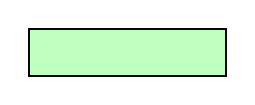
\begin{tikzpicture}[scale=1.0, transform shape]
    \tikzstyle{every node} = [draw, shape = rectangle, node distance=0mm, minimum width=4mm, minimum height=6mm, fill=green!25!white]
    \node[draw=black, thick, minimum width=25mm] (channel1) {};
\end{tikzpicture}
};
    \draw (5, 4.2) node {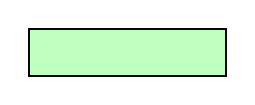
\begin{tikzpicture}[scale=1.0, transform shape]
    \tikzstyle{every node} = [draw, shape = rectangle, node distance=0mm, minimum width=4mm, minimum height=6mm, fill=green!25!white]
    \node[draw=black, thick, minimum width=25mm] (channel1) {};
\end{tikzpicture}
};
    \draw (5, 3.5) node {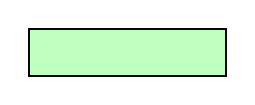
\begin{tikzpicture}[scale=1.0, transform shape]
    \tikzstyle{every node} = [draw, shape = rectangle, node distance=0mm, minimum width=4mm, minimum height=6mm, fill=green!25!white]
    \node[draw=black, thick, minimum width=25mm] (channel1) {};
\end{tikzpicture}
};
    \draw (5, 2.8) node {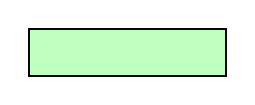
\begin{tikzpicture}[scale=1.0, transform shape]
    \tikzstyle{every node} = [draw, shape = rectangle, node distance=0mm, minimum width=4mm, minimum height=6mm, fill=green!25!white]
    \node[draw=black, thick, minimum width=25mm] (channel1) {};
\end{tikzpicture}
};%[label=below:{\tiny \(n\) spectrum channels}]
    \draw (5, 1.25) node {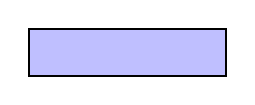
\begin{tikzpicture}[scale=1.0, transform shape]
    \tikzstyle{every node} = [draw, shape = rectangle, node distance=0mm, minimum width=4mm, minimum height=6mm, fill=blue!25!white]
    \node[draw=black, thick, minimum width=25mm] (channel1) {};
\end{tikzpicture}
};%[label=below:{\tiny dedicated control channel}]
\end{tikzpicture}


\chapter{Proposed Methodology: Feedback-based Multi-radio Exploitation Approach}\label{chap:feedback}

Our proposed approach consists of mainly two different types of feedbacks. Firstly, we measure packet transmission ratio for each radio to evaluate radio performance. Secondly, we calculate channel utilization ratio for each channel to assess corresponding channel condition.

\section{Overview of The Proposed Approach}

We present a brief overview of our proposed feedback-based approach in \cref{fig:overview}. As SUs are equipped with multiple radios, a single radio is first selected to send an application layer packet. The radio selection process as described in \cref{sec:radioSelect} is based on packet transmission ratio. The selected radio then senses the PU activity on its current channel. If the current channel is idle, it transmits the packet following an standard CSMA-CA protocol. However, if the current channel is busy, then the radio selects another channel and starts switching to that channel. The channel selection process is based on channel utilization ratio and is described in \cref{sec:channelSelect}.

\iffalse
\begin{figure}[!htb]
\begin{center}
%\resizebox{0.625\textwidth}{!}{
\begin{center}

\end{center}
%}
\caption{High-level overview of the proposed approach}
\label{fig:overview}
\end{center}
\end{figure}
\fi

\begin{figure}[!htb]
\begin{center}
\begin{tikzpicture}[scale=1.0, transform shape]
    \node {\begin{tikzpicture}[node distance=2cm, scale=1.0, transform shape]
\tikzset{every node/.style={text width=4cm}}
\tikzstyle{startstop} = [rectangle, rounded corners, minimum width=3cm, minimum height=1cm,text centered, draw=black, fill=red!30]
\tikzstyle{io} = [trapezium, trapezium left angle=70, trapezium right angle=110, minimum width=3cm, minimum height=1cm, text centered, draw=black, fill=blue!30]
\tikzstyle{process} = [rectangle, minimum width=3cm, minimum height=1cm, text centered, draw=black, fill=orange!30]
\tikzstyle{decision} = [diamond, minimum width=1cm,  text badly centered, inner sep=0pt, draw=black, fill=green!30]
\tikzstyle{arrow} = [thick,->,>=stealth]
\node (sendPacket) [startstop] {Transport layer packet is sent to the SU agent, \texttt{sendPacket}};
\node (getSelectedRadio) [process, below of=sendPacket] {SU agent selects a radio to transmit the packet, \texttt{getSelectedRadio}};
\node (startSensing) [decision, text width=3cm, aspect=2, below of=getSelectedRadio, yshift=-1cm] {Radio senses PU's activities, \texttt{startSensing}};
\node (startSwitching) [process, text width=3.5cm, below right =0.75cm and -0.625 cm of startSensing, xshift=-0.5cm] {Radio switches its channel, \texttt{startSwitching}};
%right of=startSensing, yshift=-3cm
\node (getSelectedChannel) [process, below=0.65cm of startSwitching, xshift=-0.25cm] {SU agent selects a channel for radio, \texttt{getSelectedChannel}};
\node (transmitPacket) [process, text width=3.5cm, below left =0.75cm and -0.625 cm of startSensing] {Radio transmits the packet, \texttt{transmitPacket}};
\node (endTransmit) [decision, text width=3cm, aspect=2, below=0.5cm of transmitPacket] {Transmission end?};
\node (end) [startstop, text width=0.5cm, below of=endTransmit] {End};
\draw [arrow] (sendPacket) -- (getSelectedRadio);
\draw [arrow] (getSelectedRadio) -- (startSensing);
\draw [arrow] (transmitPacket) -- (endTransmit);
\draw [arrow] (endTransmit) -- (end);
\node at (-3, -10) {No};
\node at (-1.4, -10.75) {Yes};
\node at (-1.75, -5) {Idle};
\node at (5.2, -5) {Busy};
\draw [arrow] (-4.9,-9.575) -- (-6,-9.575) -- (-6, -3.35) -- (0, -3.35);
\draw [arrow] (-2.8,-5) -- (-3,-5) -- (-3,-6.475);
\draw [arrow] (2.8,-5) -- (3,-5) -- (3,-6.475);
\draw [arrow] (3,-8.025) --  (3,-8.675);
\draw [arrow] (4.05,-9.575) -- (5.2,-9.575) -- (5.2, -3.35) -- (0, -3.35);
\end{tikzpicture}
};
\end{tikzpicture}
\caption{High-level overview of the proposed approach}
\label{fig:overview}
\end{center}
\end{figure}

\section{Radio Selection Based on Packet Transmission Ratio}
\label{sec:radioSelect}

When SUs are equipped with multiple data transmission radios, the first issue comes into play is to select the radio for transmitting data packets. For this selection, our proposed approach maintains two counters for each radio namely \texttt{pktQueued} denoting the number of packets queued for the radio and \texttt{pktSent} denoting the number of packets already transmitted by the radio. Whenever the Application layer of an SU sends a packet for transmission to the lower layers, the secondary user agent calculates the ratio between 	\texttt{pktSent} and \texttt{pktQueued} for each radio. We define the ratio as Packet Transmission Ratio, \texttt{sentQueuedRatio}. Subsequently, we normalize values of the ratio to rank the radios in a uniform manner. A larger value of such packet transmission ratio implies that the corresponding radio has been successful to transmit more packets than others. Using these packet transmission ratios as the weights, our proposed approach conducts a weighted lottery to select radios for transmission of packets.

At the beginning of the packet transmission process, an SU's radio senses its current channel. If the cognitive radio finds that the current channel is busy, then the radio starts a channel switching process. At the beginning of the channel switching process, the SU agent lists all the channels currently not used by any radio of the corresponding SU. If no such channel can be found, the radio is reported as Off and the queued packets are discarded as dropped. Otherwise, a channel is selected from the list of available channels, \texttt{availableChannels} based on current channel utilization ratio. We present the selection process along with the definition of the channel utilization ratio next.

\section{Channel Selection Based on Channel Utilization Ratio}
\label{sec:channelSelect}

In our proposed approach, each SU keeps two counters for each channel. First, \texttt{pktTransmitted} counts the number of packets transmitted in the channel by the corresponding SU radios. Besides, \texttt{pktReceived} counts the number of packets successfully received by the corresponding receiver. The counter, \texttt{pktReceived} is incremented after reception of each acknowledgment packet. When a switching radio requires selecting a channel among \texttt{availableChannels}, the SU agent calculates the ratio between \texttt{pktReceived} and \texttt{pktTransmitted} for each channel on the list, \texttt{availableChannels}. We define the ratio as Channel Utilization Ratio, \texttt{RxTxRatio}. We normalize this ratio to rank the channels in a uniform manner. Using these channel utilization ratios as the weights, the SU agent conducts a weighted lottery to select the channel to switch over.

The last two important aspects of our feedback-based multi-radio exploitation approach are the reactivation of Off radios and probabilistic channel switching. Radios marked Off at the beginning of a channel switching process, are reactivated probabilistically by the radio selection process. While calculating packet transmission ratio from \texttt{pktSent} and \texttt{pktQueued}, in the case of Off radios, the ratio is multiplied by \texttt{wakeUpProbability} to make it less likely to be selected as the next radio for sending a packet. Though, if selected, the Off radio is reported as On and it starts its cognitive cycle through the channel sensing process. The probabilistic channel switching implies that radios do not always switch after finding their current channel busy. The channel switching process occurs at a probability of \texttt{switchingProbability}.

\begin{algorithm}
\caption{$\mathit{sendPacket}$: SU agent sending a packet, $p$}
\label{alg:sendPacket}
\begin{algorithmic}[1]
\Function{$\mathit{sendPacket}$}{}
\State $\mathit{radioIndex}\gets \mathit{getSelectedRadio}()$
\State $pktQueued[radioIndex]\gets $\Statex$ 1+\mathit{pktQueued}[\mathit{radioIndex}]$
\State $\mathit{radioStatus}[\mathit{radioIndex}]\gets \mathit{On}$
\State $\mathit{startSensing}(\mathit{radioIndex})$
\EndFunction
\end{algorithmic}
\end{algorithm}

\begin{algorithm}
\caption{$\mathit{startSensing}$: SU's radio sensing its channel}
\label{alg:startSensing}
\begin{algorithmic}[1]
\Function{$\mathit{startSensing}$}{$\mathit{radioIndex}$}
\If{$\mathit{currentChannel}[\mathit{radioIndex}]$ is $\mathit{Busy}$}
\State $\mathit{startSwitching}(\mathit{radioIndex})$
\Else
\State $\mathit{transmitPacket}(\mathit{radioIndex})$
\EndIf
\EndFunction
\end{algorithmic}
\end{algorithm}

\begin{algorithm}
\caption{$\mathit{startSwitching}$: SU's radio changing its channel}\label{alg:startSwitching}
\begin{algorithmic}[1]
\Function{$\mathit{startSwitching}$}{$\mathit{radioIndex}$}
\State Stop the switching process and \textbf{return} with the probability $(1-\mathit{switchingProbability})$
\State $\mathit{availableChannels} \gets $ all the channels currently not used by any radio of the SU
\If{$\mathit{availableChannels}=\varnothing$}
\State $\mathit{radioStatus}[\mathit{radioIndex}]\gets \mathit{Off}$
\State $\mathit{dropPacket}()$
\Else
\State $\mathit{channelIndex}\gets$\Statex$ \mathit{getSelectedChannel}(\mathit{availableChannels})$
\State $\mathit{currentChannel}[\mathit{radioIndex}] \gets \mathit{channelIndex}$
\State $\mathit{channels}[\mathit{channelIndex}] \gets \mathit{Used}$
\State $\mathit{startSensing}(\mathit{radioIndex})$
\EndIf
\EndFunction
\end{algorithmic}
\end{algorithm}

\begin{algorithm}
\caption{$\mathit{transmitPacket}$: SU's radio transmitting a packet, $p$}
\label{alg:transmitPacket}
\begin{algorithmic}[1]
\Function{$\mathit{transmitPacket}$}{$\mathit{radioIndex}$}
\State $\mathit{pktSent}[\mathit{radioIndex}]\gets \mathit{pktSent}[\mathit{radioIndex}]+1$
\State $\mathit{pktTransmitted}[\mathit{currentChannel}[\mathit{radioIndex}]]\gets$\par\hskip\algorithmicindent$\mathit{pktTransmitted}[\mathit{currentChannel}[\mathit{radioIndex}]]$\par\hskip\algorithmicindent$+1$
\State encapsulate $\mathit{radioIndex}$ within the packet, $p$ and transmit it following CSMA-CA
\EndFunction
\end{algorithmic}
\end{algorithm}
\begin{algorithm}
\caption{$\mathit{receiveAckPacket}$: SU's radio receiving an Ack packet, $p$}
\label{alg:receivePacket}
\begin{algorithmic}[1]
\Function{$\mathit{receivePacket}$}{$p$}
\State $\mathit{radioIndex} \gets $ the radio index extracted from the packet
\If{$\mathit{radioIndex}=$ current radio's index}
\State $\mathit{pktReceivedRadio}[\mathit{radioIndex}]\gets$\Statex$ \mathit{pktReceivedRadio}[\mathit{radioIndex}]+1$
\State $\mathit{pktReceived}[\mathit{currentChannel}[\mathit{radioIndex}]]\gets$\Statex$ \mathit{pktReceived}[\mathit{currentChannel}[\mathit{radioIndex}]]+1$
\EndIf
\EndFunction
\end{algorithmic}
\end{algorithm}

\begin{algorithm}
\caption{$\mathit{getSelectedRadio}$: Selects an SU radio to send a packet}
\label{alg:getSelectedRadio}
\begin{algorithmic}[1]
\Function{$\mathit{getSelectedRadio}$}{}
%\State $\mathit{radios} \gets$ all the radios
\State $k \gets$ the number of radios
\State $\mathit{sentQueuedRatio} [0\ldots k] \gets $a new array of floating point values
\State $\mathit{total} \gets 0.0$
\For{$r=1$ \textbf{to} $k$}
\State $\mathit{sentQueuedRatio}[r] \gets \dfrac{(1+\mathit{pktSent}[\mathit{r}])}{(1+\mathit{pktQueued}[\mathit{r}])}$
\If{$\mathit{radioStatus}[\mathit{r}]=\mathit{Off}$}
\State $\mathit{sentQueuedRatio}[r] \gets$\Statex[2]$ \mathit{sentQueuedRatio}[r] \times \mathit{wakeUpProbability}$
\EndIf
\State $\mathit{total} \gets \mathit{total} + \mathit{sentQueuedRatio}[r]$
\EndFor
\For{$r=1$ \textbf{to} $k$}
\State $\mathit{sentQueuedRatio}[r] \gets \dfrac{\mathit{sentQueuedRatio}[r]}{\mathit{total}}$
\EndFor
\State $\mathit{radioIndex} \gets$ winner of the weighted lottery among all the radios with weight, $\mathit{sentQueuedRatio}$
\State \textbf{return} $\mathit{radioIndex}$
\EndFunction
\end{algorithmic}
\end{algorithm}

\begin{algorithm}
\caption{$\mathit{getSelectedChannel}$: Selects a new channel to switch for an SU radio over the $\mathit{availableChannels}$}
\label{alg:getSelectedRadio}
\begin{algorithmic}[1]
\Function{$\mathit{getSelectedChannel}$}{$\mathit{availableChannels}$}
\State $k \gets$ the number of channels in $\mathit{availableChannels}$
\State $\mathit{RxTxRatio} [0\ldots k] \gets $ a new array of floating point values
\State $\mathit{total} \gets 0.0$
\For{$r=1$ \textbf{to} $k$}
\State $\mathit{RxTxRatio}[r] \gets \dfrac{(1+\mathit{pktReceived}[\mathit{r}])}{(1+\mathit{pktTransmitted}[\mathit{r}])}$
\State $\mathit{total} \gets \mathit{total} + \mathit{RxTxRatio}[r]$
\EndFor
\For{$r=1$ \textbf{to} $k$}
\State $\mathit{RxTxRatio}[r] \gets \dfrac{\mathit{RxTxRatio}[r]}{\mathit{total}}$
\EndFor
\State $\mathit{channelIndex} \gets$ winner of the weighted lottery among all the channels in $\mathit{availableChannels}$ with weight, $\mathit{RxTxRatio}$
\State \textbf{return} $\mathit{channelIndex}$
\EndFunction
\end{algorithmic}
\end{algorithm}

\section{Variants of Our Proposed Approach}

We create three variants of our proposed approach introducing radio and channel selection based on a random variable following a uniform distribution. While selecting the next radio for data packet transmission, we can randomly select any one of data radios ignoring the packet transmission ratios. Similarly, the next channel to switch can also be chosen randomly from the available channels irrespective of the channel utilization ratio. We define this random radio and channel selection policy as unweighted lottery. From this unweighted lottery, we devise three variants of our proposed approach as described in \cref{tab:variantDefintion}. The approach of randomly selecting both the radio and the channel has not be listed as the variants of the proposed approach as that approach is quite similar to the approach proposed by Zhong et al.,~\cite{zhong2014capacity}.

\begin{table*}
\begin{center}
  \caption{Several variants of the proposed feedback-based approach}
  \label{tab:variantDefintion}
  \begin{tabular}{p{0.2\textwidth}p{0.35\textwidth}p{0.35\textwidth}}
    \toprule
    Variant name & Radio selection policy & Channel selection policy\\
    \midrule
    Radio feedback & Weighted lottery based on radio transmission ratio & Unweighted lottery \\
    Channel feedback & Unweighted lottery  & Weighted lottery based on channel utilization ratio \\
    Radio channel feedback & Weighted lottery based on radio transmission ratio & Weighted lottery based on channel utilization ratio \\
    \bottomrule
  \end{tabular}
\end{center}
\vspace{-0.8cm}
\end{table*}
\endinput


\chapter{Experimental Evaluation}
\label{chap:results}

Our proposed system requires wireless devices with multiple networking interface modules. Each of these modules must also have cognitive capability to ensure the basic requirements of our proposed architecture. The development of such devices involves a highly complex level of sophistication and fabrication. Such a development of cognitive radio networks in real setup is still under research. Therefore, we evaluate the performance of our proposed feedback-based multi-radio exploitation approach through extensive discrete-event simulation using \texttt{ns-3}. Yet, we have to make several modifications on the \texttt{ns-3} simulator to evaluate our proposed approach on CMRNs.

\section{Simulator Modifications}

We implement our proposed approach on top of the Cognitive radio extension for ns-3 namely CRE-NS3~\cite{al2014simulating}. We modify the cognitive module of CRE-NS3 to incorporate our feedback-based approach. The existing cognitive module of CRE-NS3 provides three interfaces for each device namely control interface, transmitter interface, and receiver interface. The transmitter and receiver interfaces of the module emulate a real cognitive transceivers. Therefore, we introduce the functionality of varying number of cognitive transceivers through varying the number of the transmitter and receiver interfaces.

To implement this functionality, we utilize the \texttt{Callback} mechanism of \texttt{ns-3} extensively. Using this mechanism, we make sure that our counters (\texttt{pktQueued}, \texttt{pktSent}, \texttt{pktTransmitted}, and \texttt{pktReceived}) are incremented after corresponding events. The \texttt{Callback} mechanism has also been used to update \texttt{radioStatus}, \texttt{availableChannels}, and \texttt{currentChannel} lists.

 We also employ \texttt{ns-3} flow tagging feature, \texttt{FlowIdTag} to encapsulate and extract extra information to and from packets. As multiple radios on a single SU node share the same upper layer address (IP address), the extra \texttt{FlowIdTag} of each packet determines the radio reference (sender and receiver), using which upper layers can distinguish among multiple radios. Moreover, we add \texttt{DelayJitterEstimationTimestampTag} to each packet to calculate delay each packet experiences.

Apart from these changes, we have also made several changes in the \texttt{wifi} module of the \texttt{ns-3} simulator. Specifically, we have modified the \texttt{YansWifiPhy}, \texttt{YansWifiChannel}, \texttt{WifiPhyStateHelper}, \texttt{RegularWifiMac}, and \texttt{WifiNetDevice} models of the \texttt{wifi} module to add the cross-layer implementation of the multi-radio functionailty.

Using the modified simulator, we implement our proposed approach and evaluate its performance on the basis of four performance metrics -- total network throughput, end-to-end delay, packet drop ratio, and application layer packet delivery ratio. Besides, we measure values of these metrics for two existing CMRN protocols and compared them against that obtained using several variants of our proposed approach. We briefly describe our simulation settings next before presenting the evaluation results.

\section{Simulation Settings}

We consider that arrival and departure of a PU follow a Poisson process~\cite{heo2008mathematical}. Accordingly, we consider an exponential distribution for both inter-arrival time and service time. Hence we adopt the mean time between two successive arrivals to be 5 seconds and the mean service time to be 2 seconds. Besides, we consider that each secondary user enables a constant bit rate application where the data transmission rate is varied from 1 Mbps to 32 Mbps. Here, each secondary user is equipped with a variable number of radios. Each of the radios consists of one transmitter interface and one receiver interface. The transmitter interface transmits data over any of the eleven orthogonal channels that conventionally operate with OFDM WiFi mode having 18Mbps data rate. For each transmitter interface or radio, we associate a drop-tail queue with a maximum capacity of 100 packets, each of 1KB in size. These interfaces have a transmission range of 130m and a sensing range of 250m. To ensure that the destination users are reachable from the source users, we place the destinations at an average distance of 80m from the sources. Maintaining such average distance, primary users and secondary users are placed randomly in an area of $500$m$\times 500$m. Here, we vary the number of secondary users from 12 to 40 with a granularity of 4. For each such settings, we perform 99 simulation iterations, each of 50 seconds, and then take average results of all the iterations. It is to be noted here that the maximum iteration count for obtaining 95\% confidence interval according to Monte Carlo Sampling~\cite{winston2000simulation} is found to be 61 in our experiment settings. 

We carefully set the tuning parameters of the proposed approach after numerous simulation trials. The channel switching probability of SU radios, \texttt{switchingProbability} was varied from 0.1 to 0.9 with a granularity of 0.05 and the reactivation probability of switched-off radios, \texttt{wakeUpProbability} was varied from 0.05 to 0.5 with a granularity of 0.05. Following these initial simulation results, we selected the value of these parameters that yielded best results in terms of throughput, delay, and packet drop ratio. The \texttt{switchingProbability} is set as 0.75 and the \texttt{wakeUpProbability} is set as 0.2. The channel sensing time for each of the cognitive radio is set as 0.01s while the channel switching time is set as 0.05s.

\section{Simulation Results and Analysis}

We start presenting our simulation results for a topology having 11 primary users and 24 secondary users. Here, we vary the application data rate from the source of a flow over secondary users from 1 Mbps to 32 Mbps. Fig.~\ref{fig:topology4T}, \ref{fig:topology4D}, and \ref{fig:topology4P} show the performance of several variants of our proposed approach and other existing approaches.

\begin{figure*}[!htbp]
    \centering
    \begin{subfigure}[t]{0.45\textwidth}
        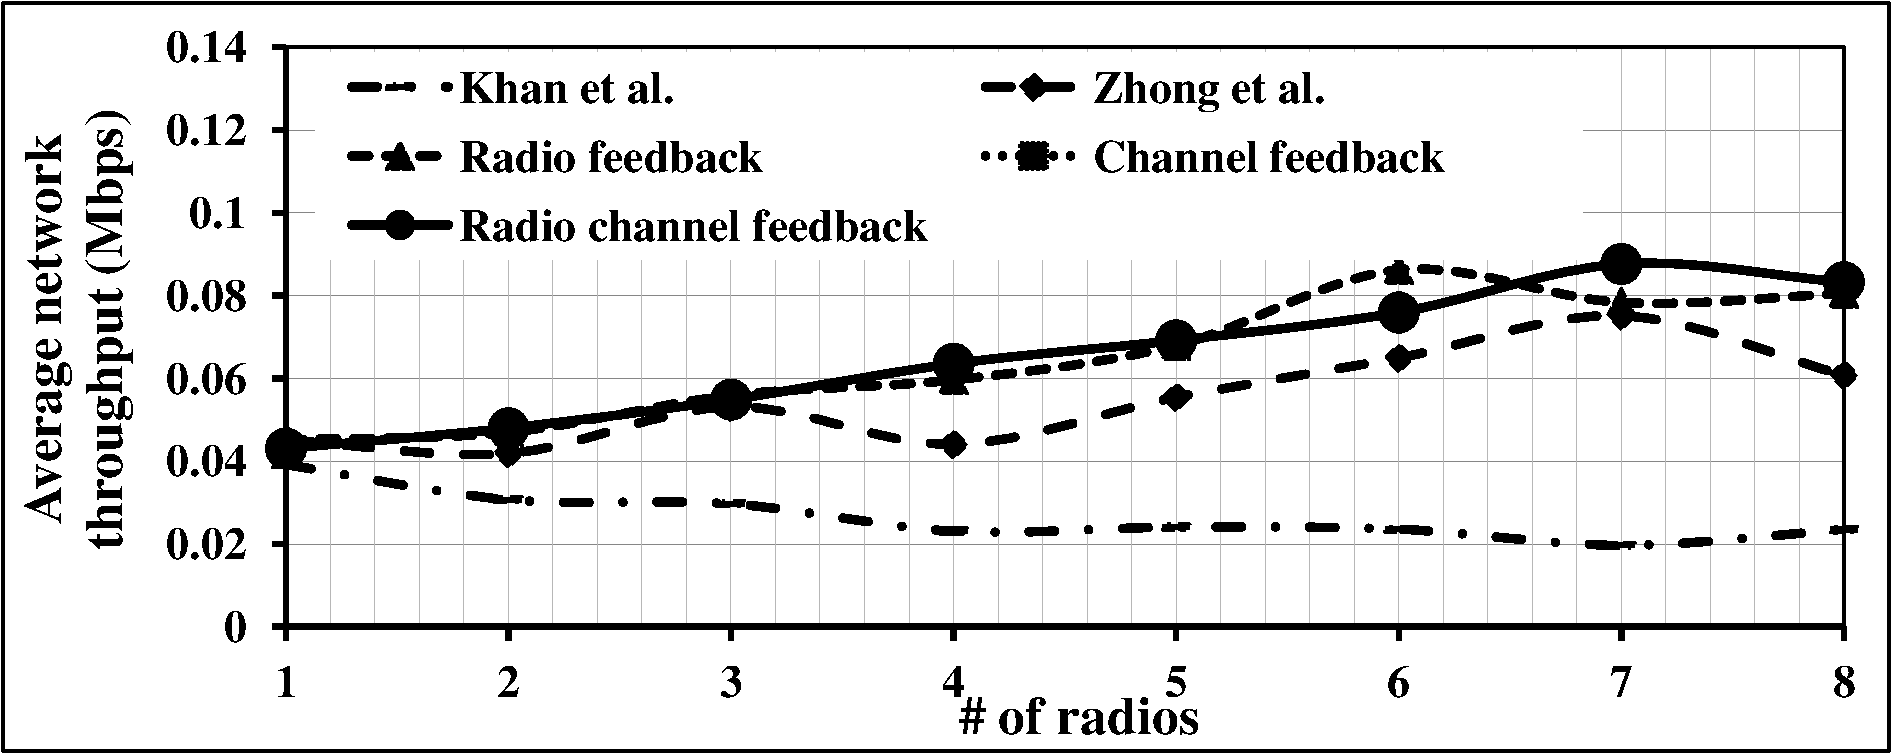
\includegraphics[width=\textwidth]{topology4/Throughput24d1}
        \caption{1Mbps application data rate}
        \label{fig:topology4T1}
    \end{subfigure}
    ~
    \begin{subfigure}[t]{0.45\textwidth}
        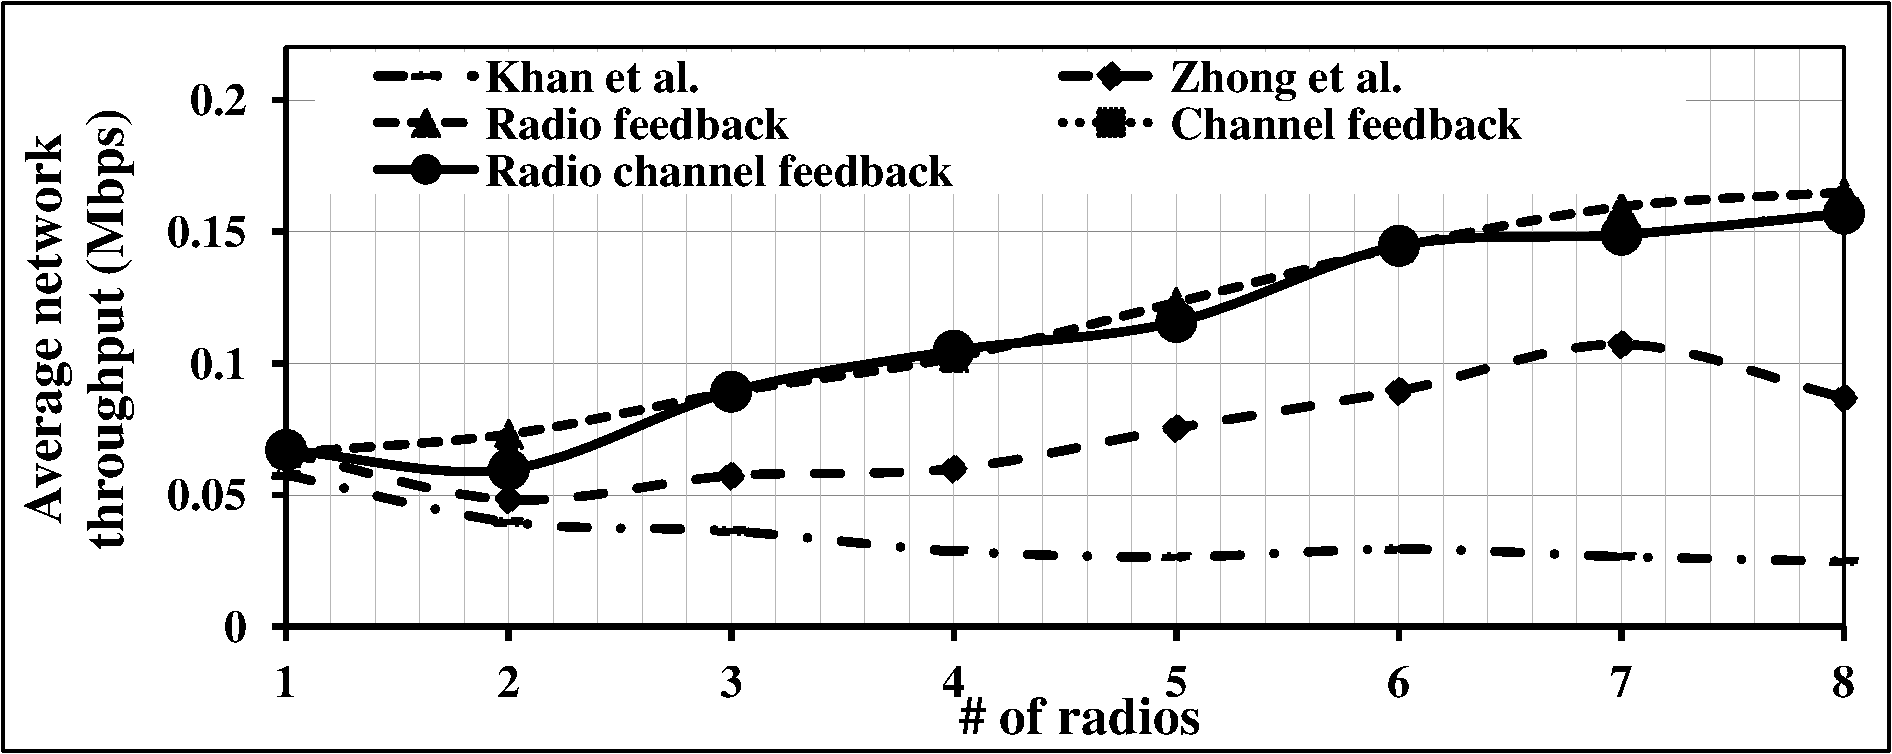
\includegraphics[width=\textwidth]{topology4/Throughput24d2}
        \caption{2Mbps application data rate}
        \label{fig:topology4T2}
    \end{subfigure}
    ~\\
    \begin{subfigure}[t]{0.45\textwidth}
        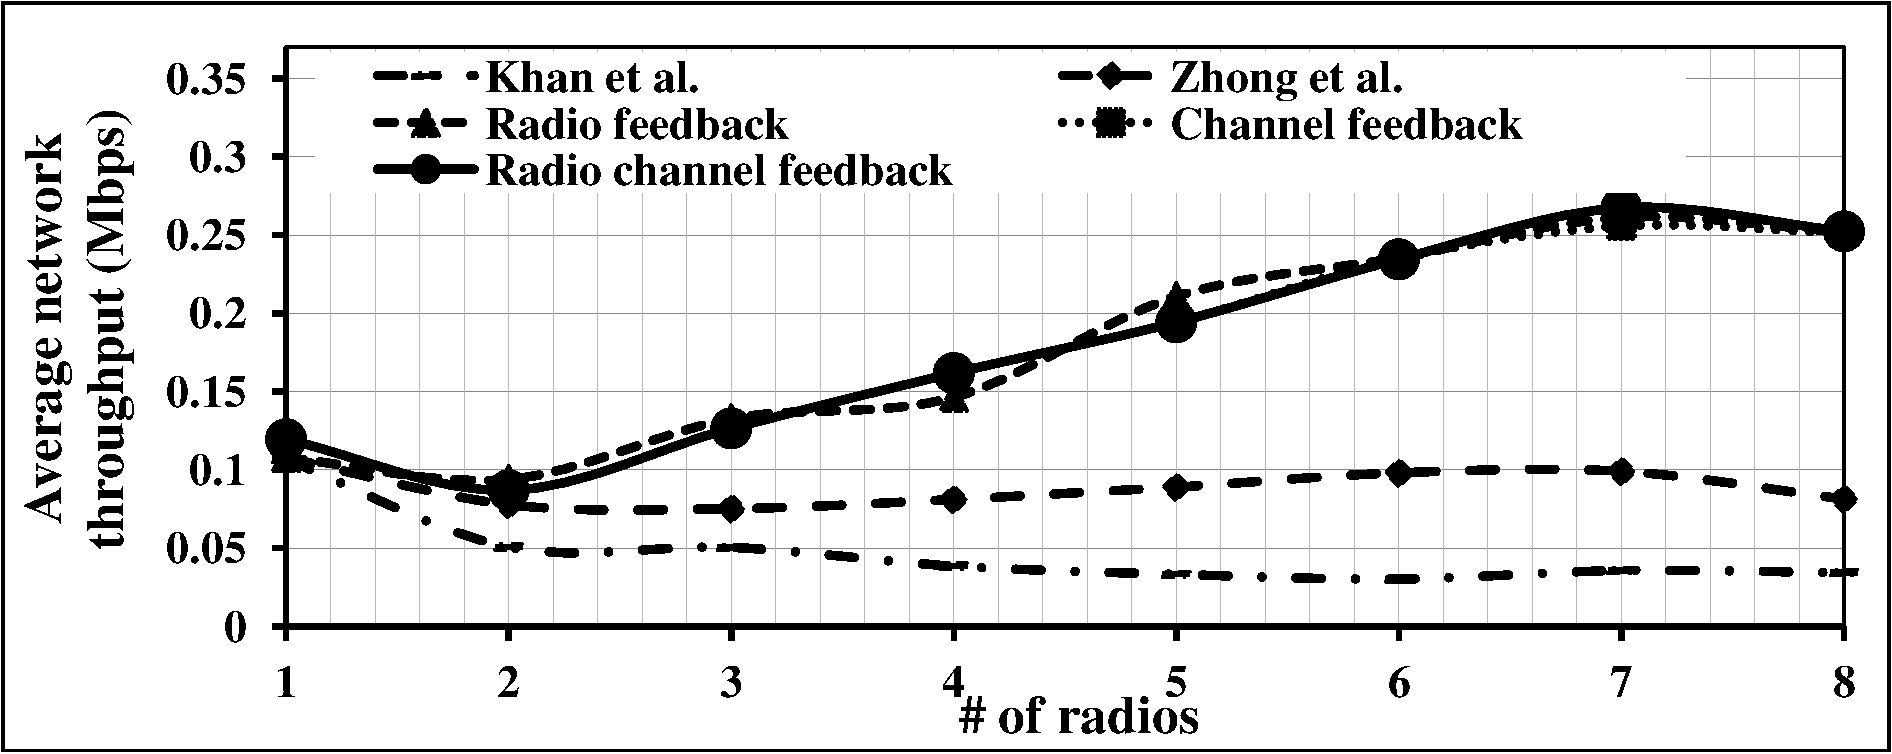
\includegraphics[width=\textwidth]{topology4/Throughput24d4}
        \caption{4Mbps application data rate}
        \label{fig:topology4T3}
    \end{subfigure}
    ~
    \begin{subfigure}[t]{0.45\textwidth}
        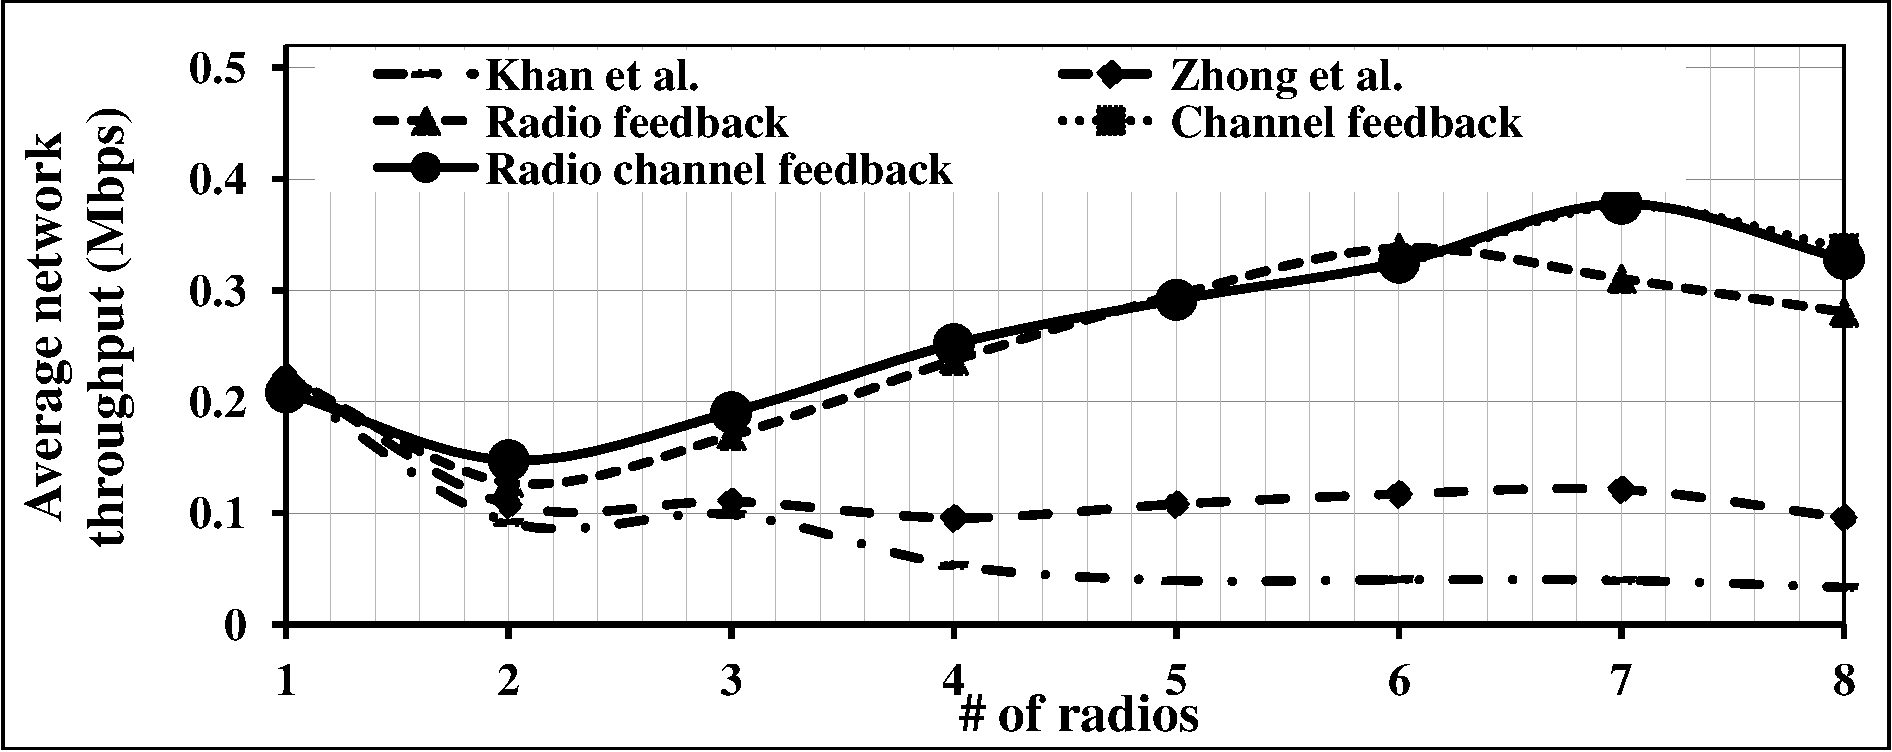
\includegraphics[width=\textwidth]{topology4/Throughput24d8}
        \caption{8Mbps application data rate}
        \label{fig:topology4T4}
    \end{subfigure}
    ~\\
    \begin{subfigure}[t]{0.45\textwidth}
        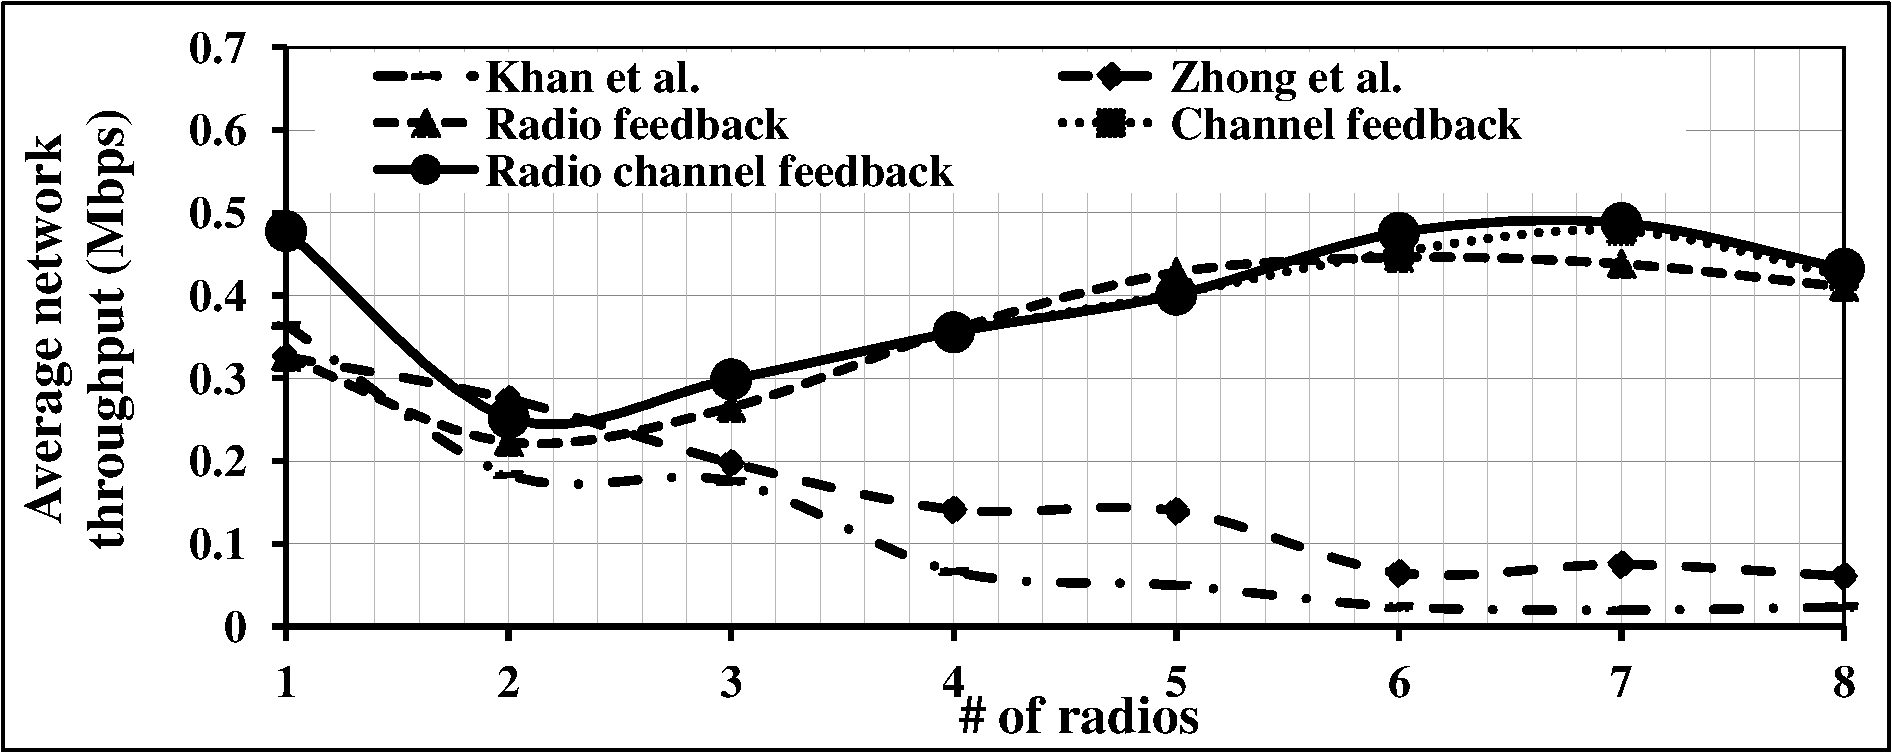
\includegraphics[width=\textwidth]{topology4/Throughput24d16}
        \caption{16Mbps application data rate}
        \label{fig:topology4T5}
    \end{subfigure}
    ~
    \begin{subfigure}[t]{0.45\textwidth}
        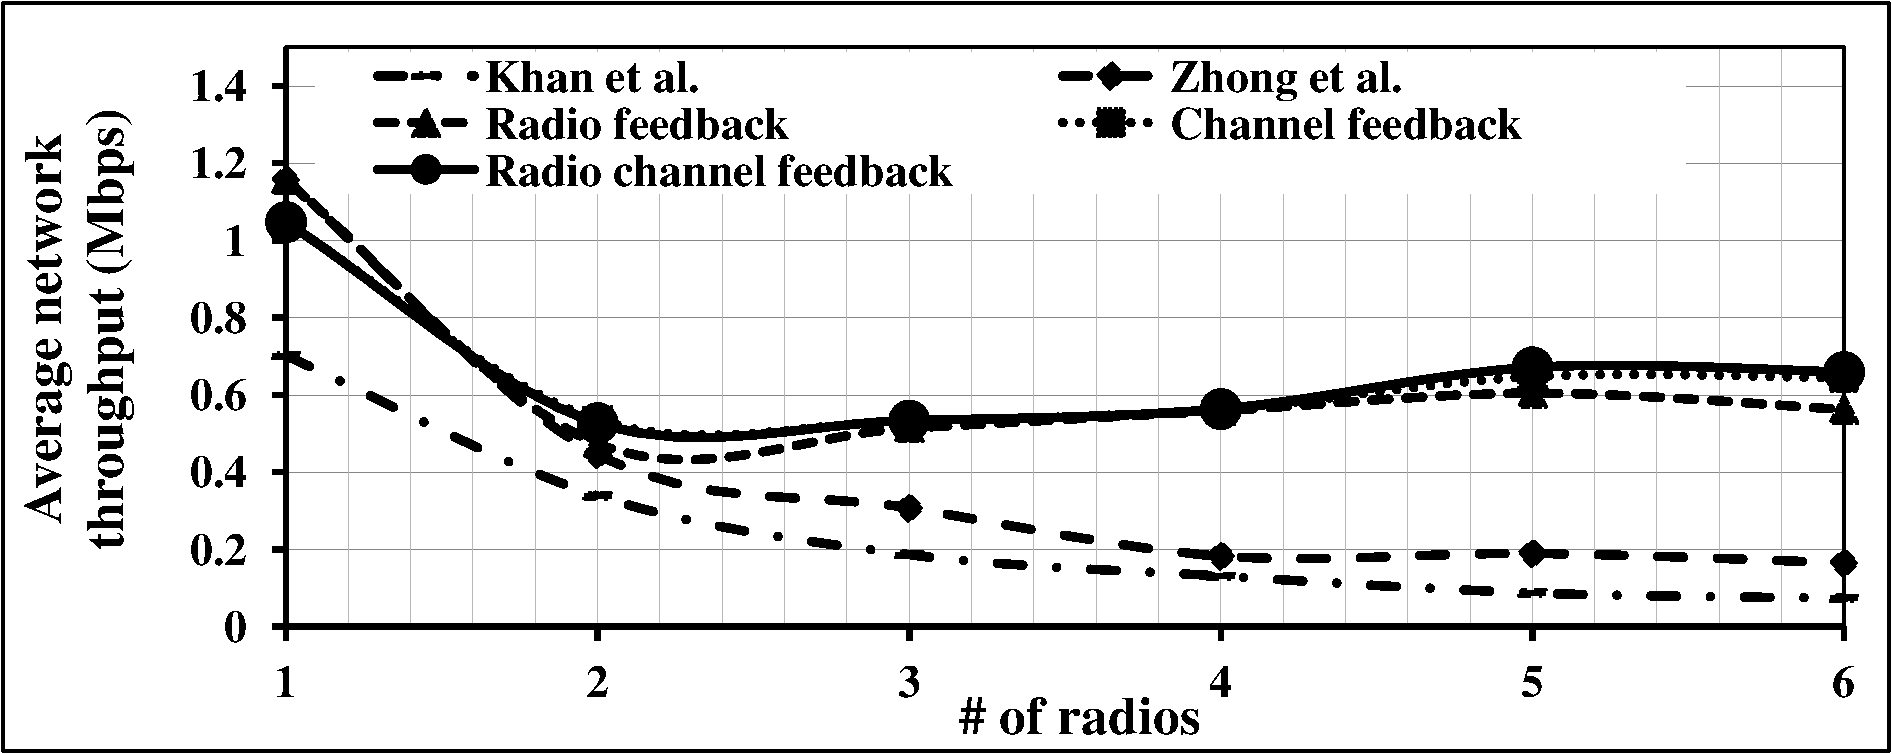
\includegraphics[width=\textwidth]{topology4/Throughput24d32}
        \caption{32Mbps application data rate}
        \label{fig:topology4T6}
    \end{subfigure}
    \caption{Average network throughput with varying number of radios for various application data rates}
    \label{fig:topology4T}
\end{figure*}

\begin{figure*}[!htbp]
    \centering
    \begin{subfigure}[t]{0.45\textwidth}
        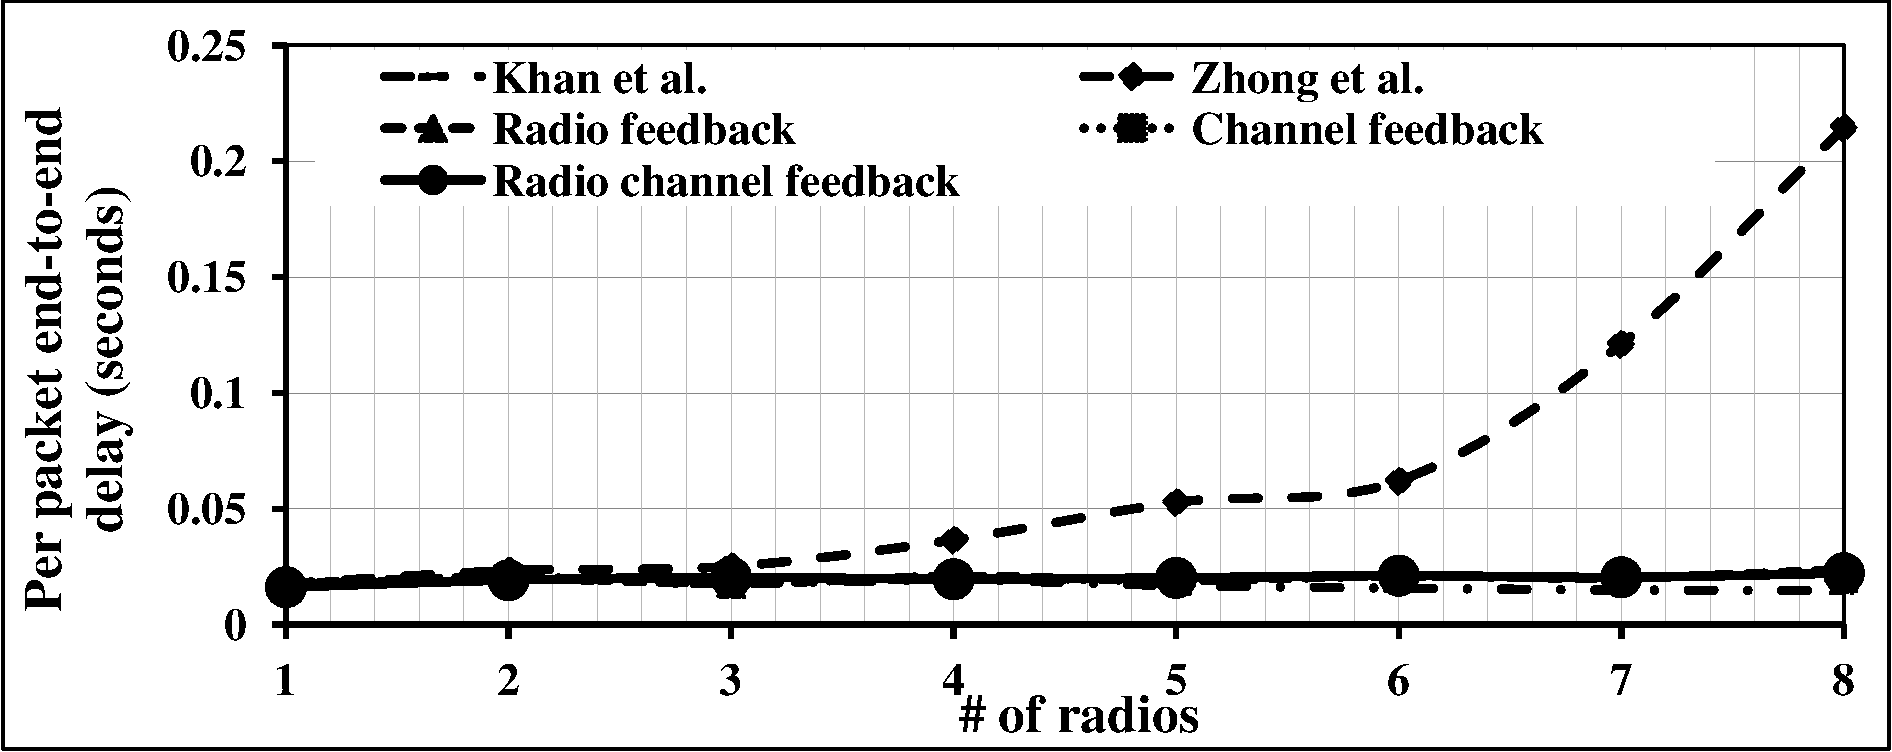
\includegraphics[width=\textwidth]{topology4/Delay24d1}
        \caption{1Mbps application data rate}
        \label{fig:topology4D1}
    \end{subfigure}
    ~
    \begin{subfigure}[t]{0.45\textwidth}
        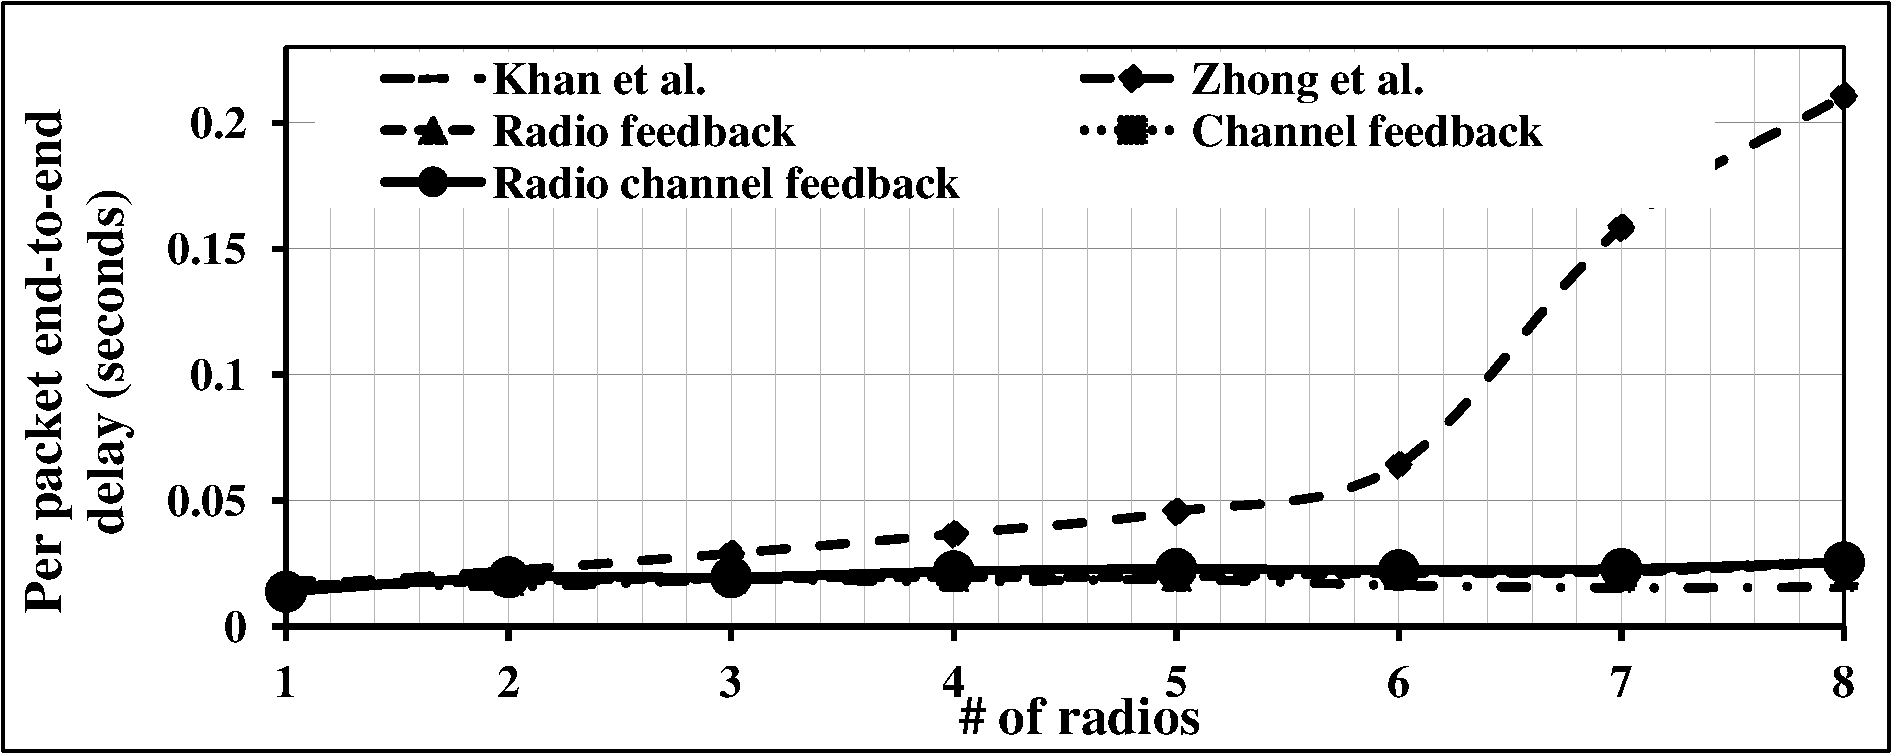
\includegraphics[width=\textwidth]{topology4/Delay24d2}
        \caption{2Mbps application data rate}
        \label{fig:topology4D2}
    \end{subfigure}
    ~\\
    \begin{subfigure}[t]{0.45\textwidth}
        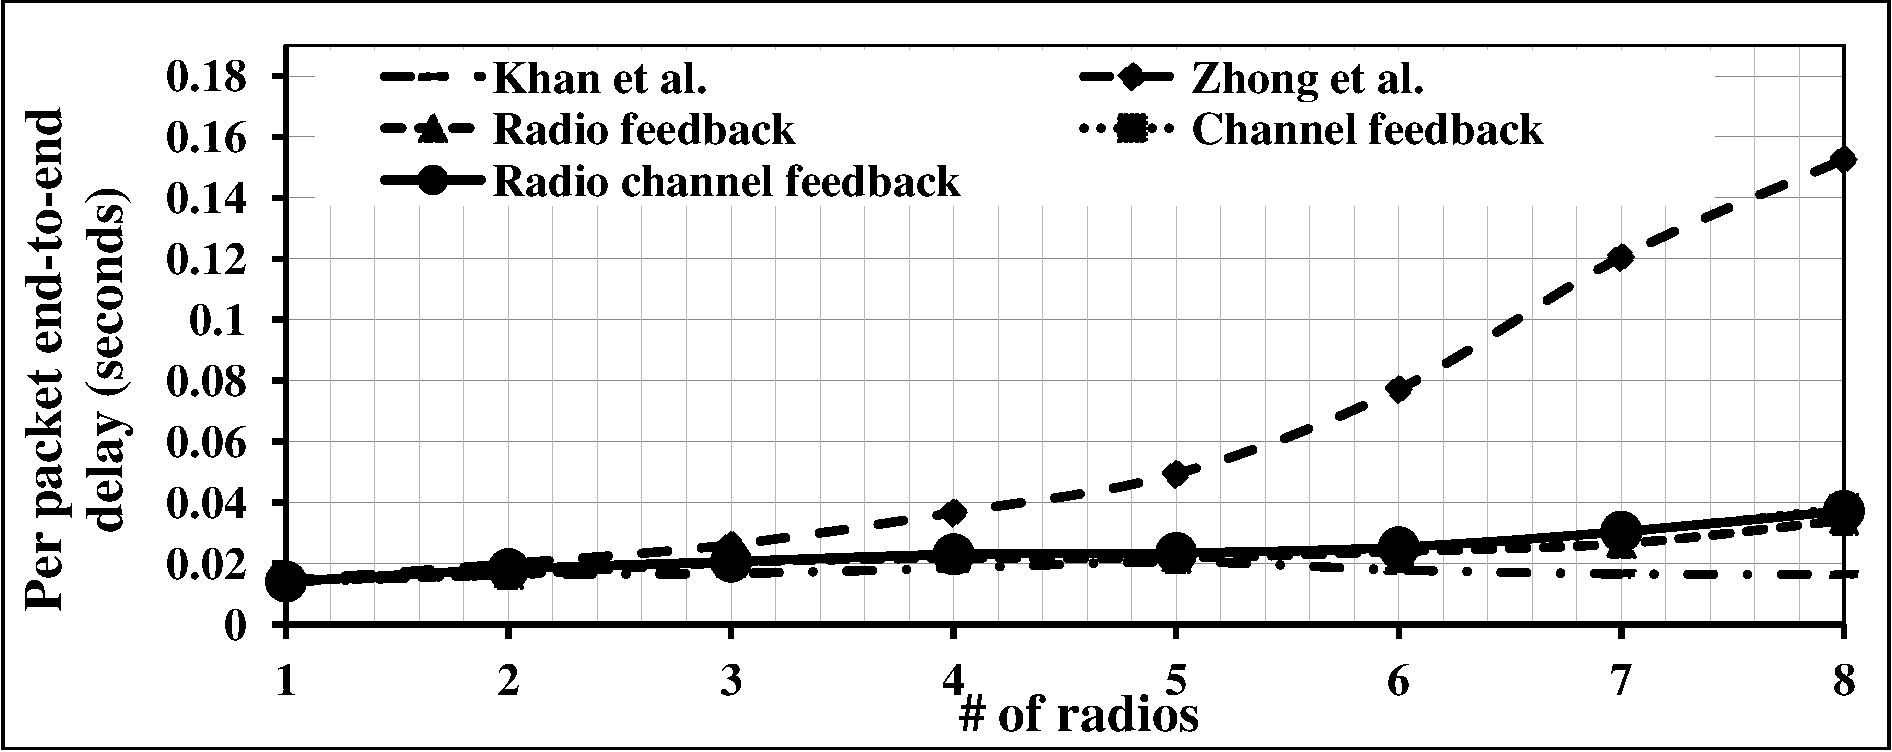
\includegraphics[width=\textwidth]{topology4/Delay24d4}
        \caption{4Mbps application data rate}
        \label{fig:topology4D3}
    \end{subfigure}
    ~
    \begin{subfigure}[t]{0.45\textwidth}
        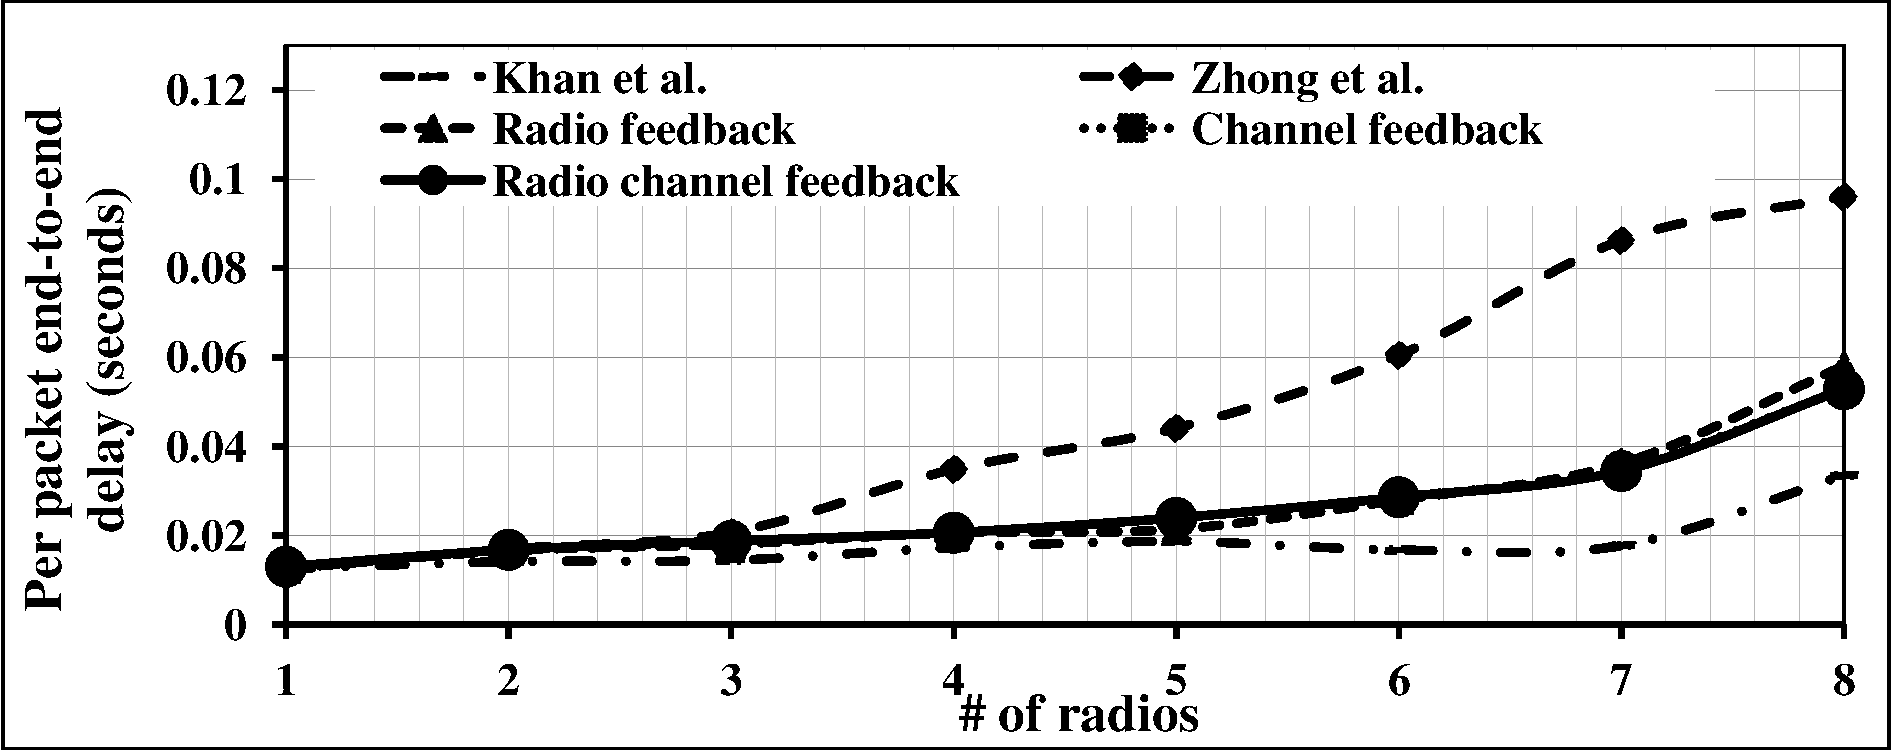
\includegraphics[width=\textwidth]{topology4/Delay24d8}
        \caption{8Mbps application data rate}
        \label{fig:topology4D4}
    \end{subfigure}
    ~\\
    \begin{subfigure}[t]{0.45\textwidth}
        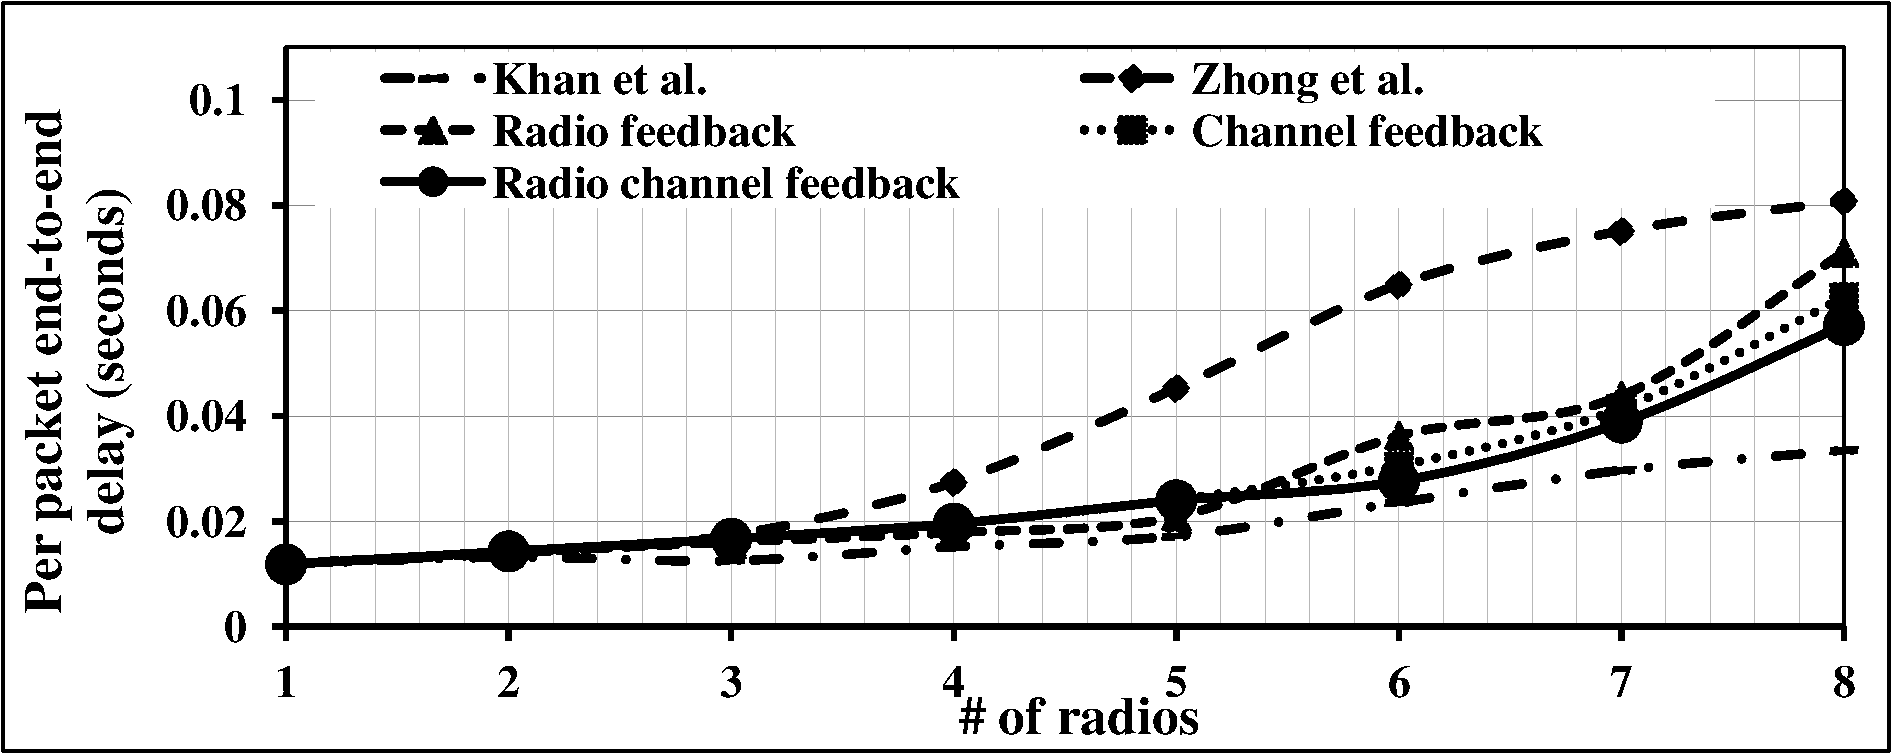
\includegraphics[width=\textwidth]{topology4/Delay24d16}
        \caption{16Mbps application data rate}
        \label{fig:topology4D5}
    \end{subfigure}
    ~
    \begin{subfigure}[t]{0.45\textwidth}
        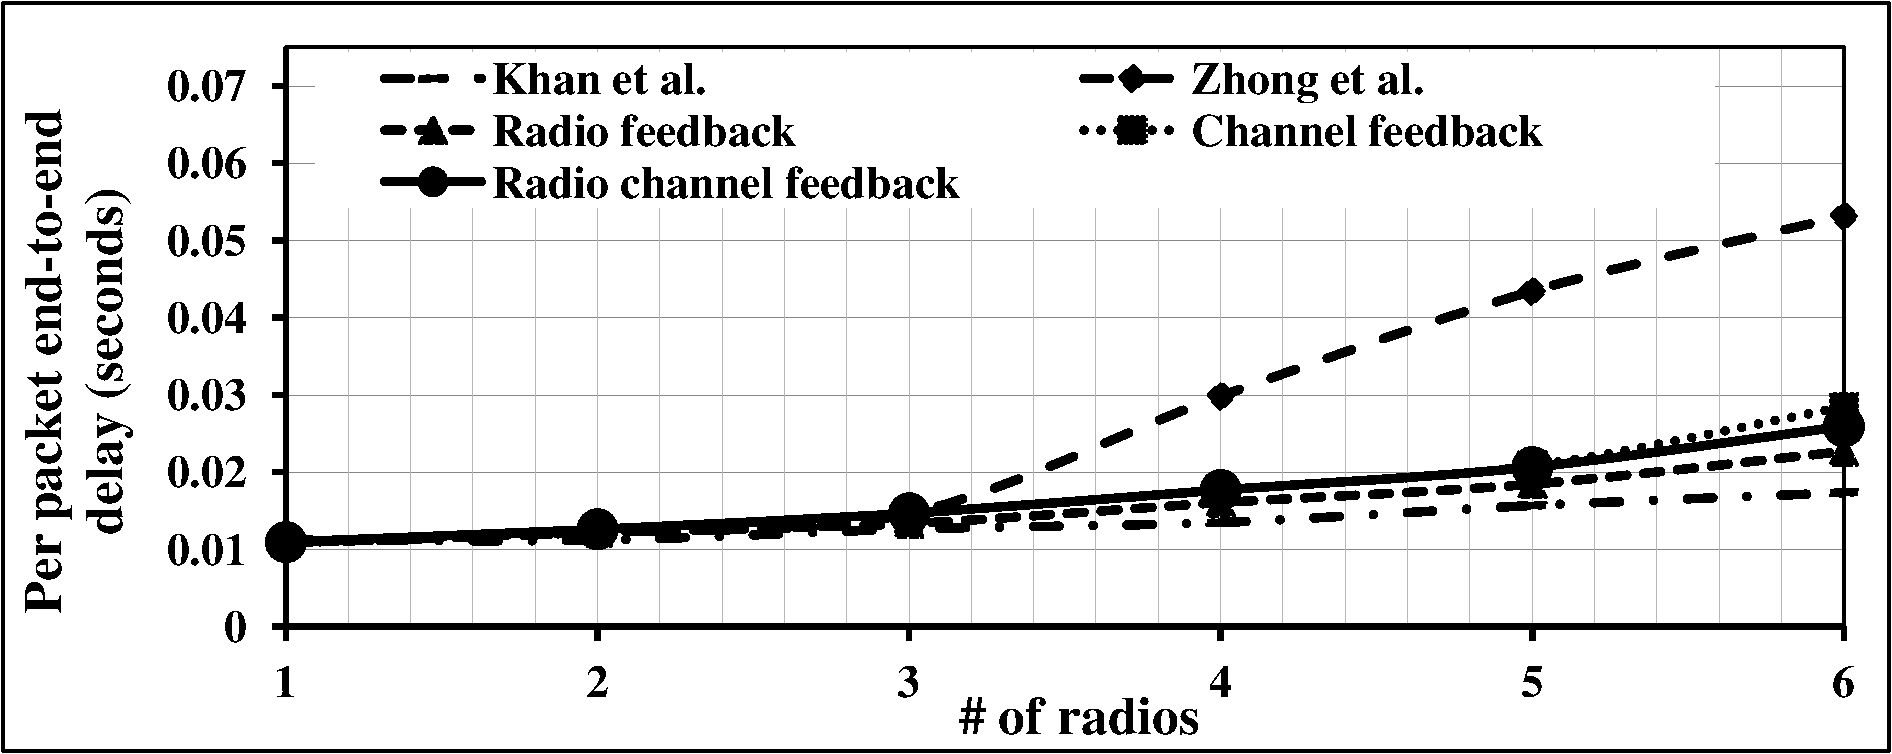
\includegraphics[width=\textwidth]{topology4/Delay24d32}
        \caption{32Mbps application data rate}
        \label{fig:topology4D6}
    \end{subfigure}
    \caption{Average end-to-end delay with varying number of radios for various application data rates}
    \label{fig:topology4D}
\end{figure*}

\begin{landscape}
\begin{figure*}[!htbp]
    \centering
    \begin{subfigure}[t]{0.625\textwidth}
        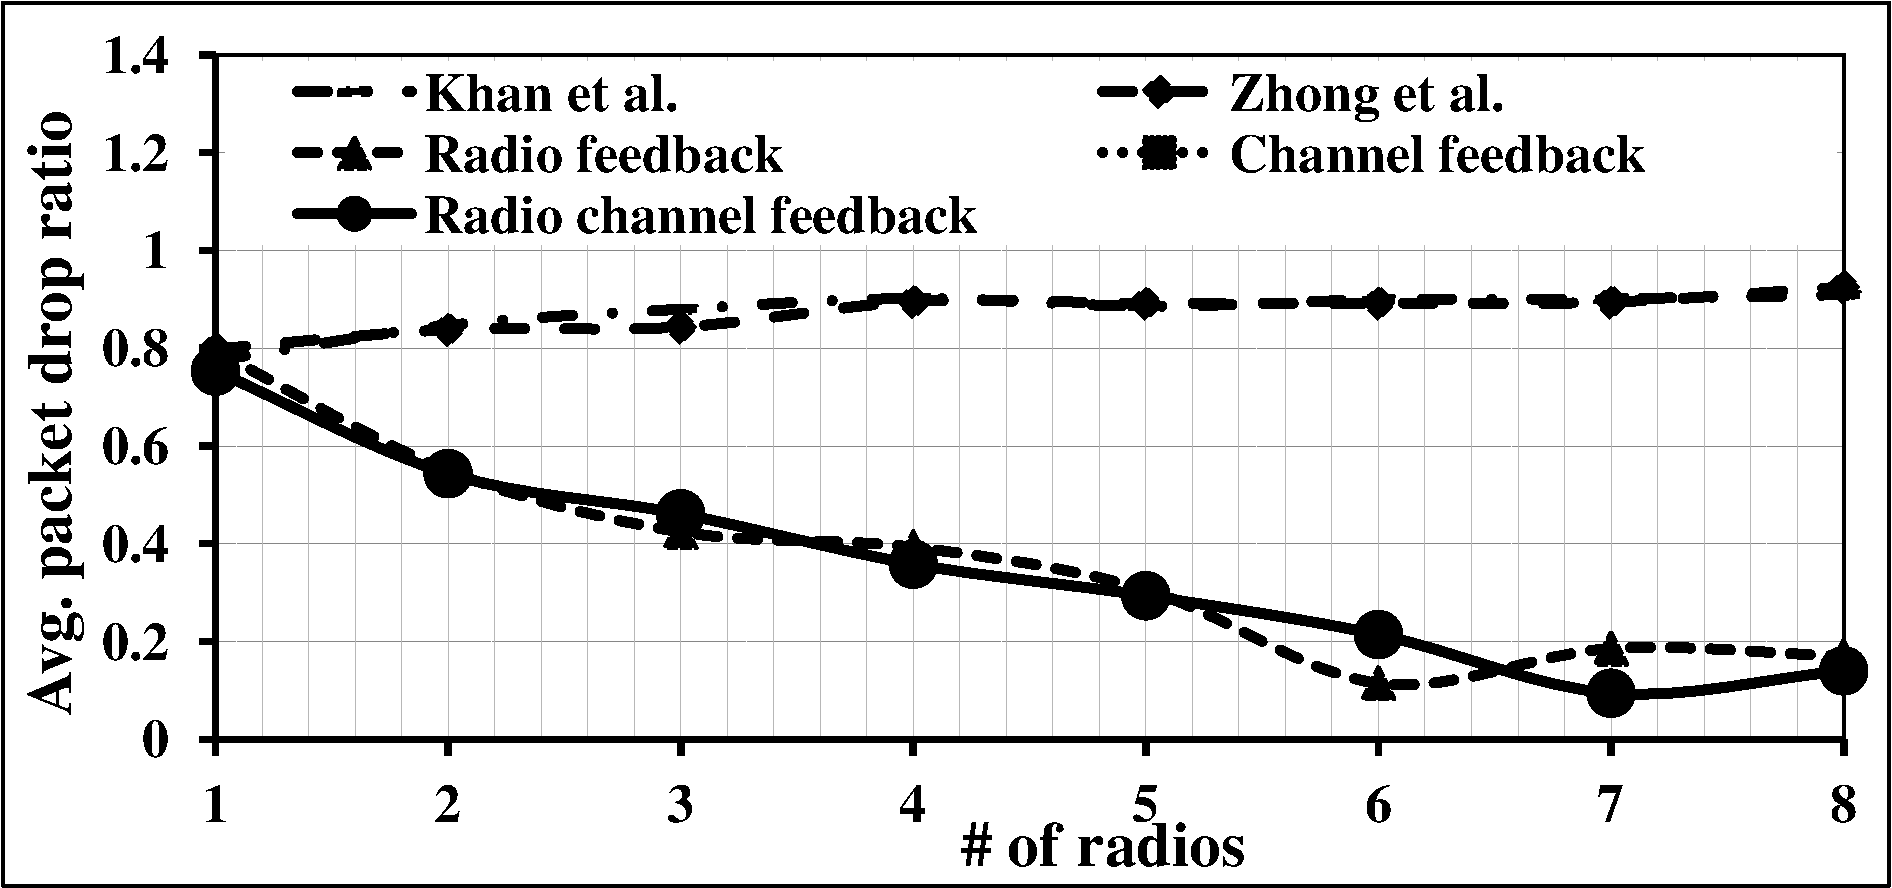
\includegraphics[width=\textwidth]{topology4/PacketDropRatio24d1}
        \caption{1Mbps application data rate}
        \label{fig:topology4P1}
    \end{subfigure}
    ~
    \begin{subfigure}[t]{0.625\textwidth}
        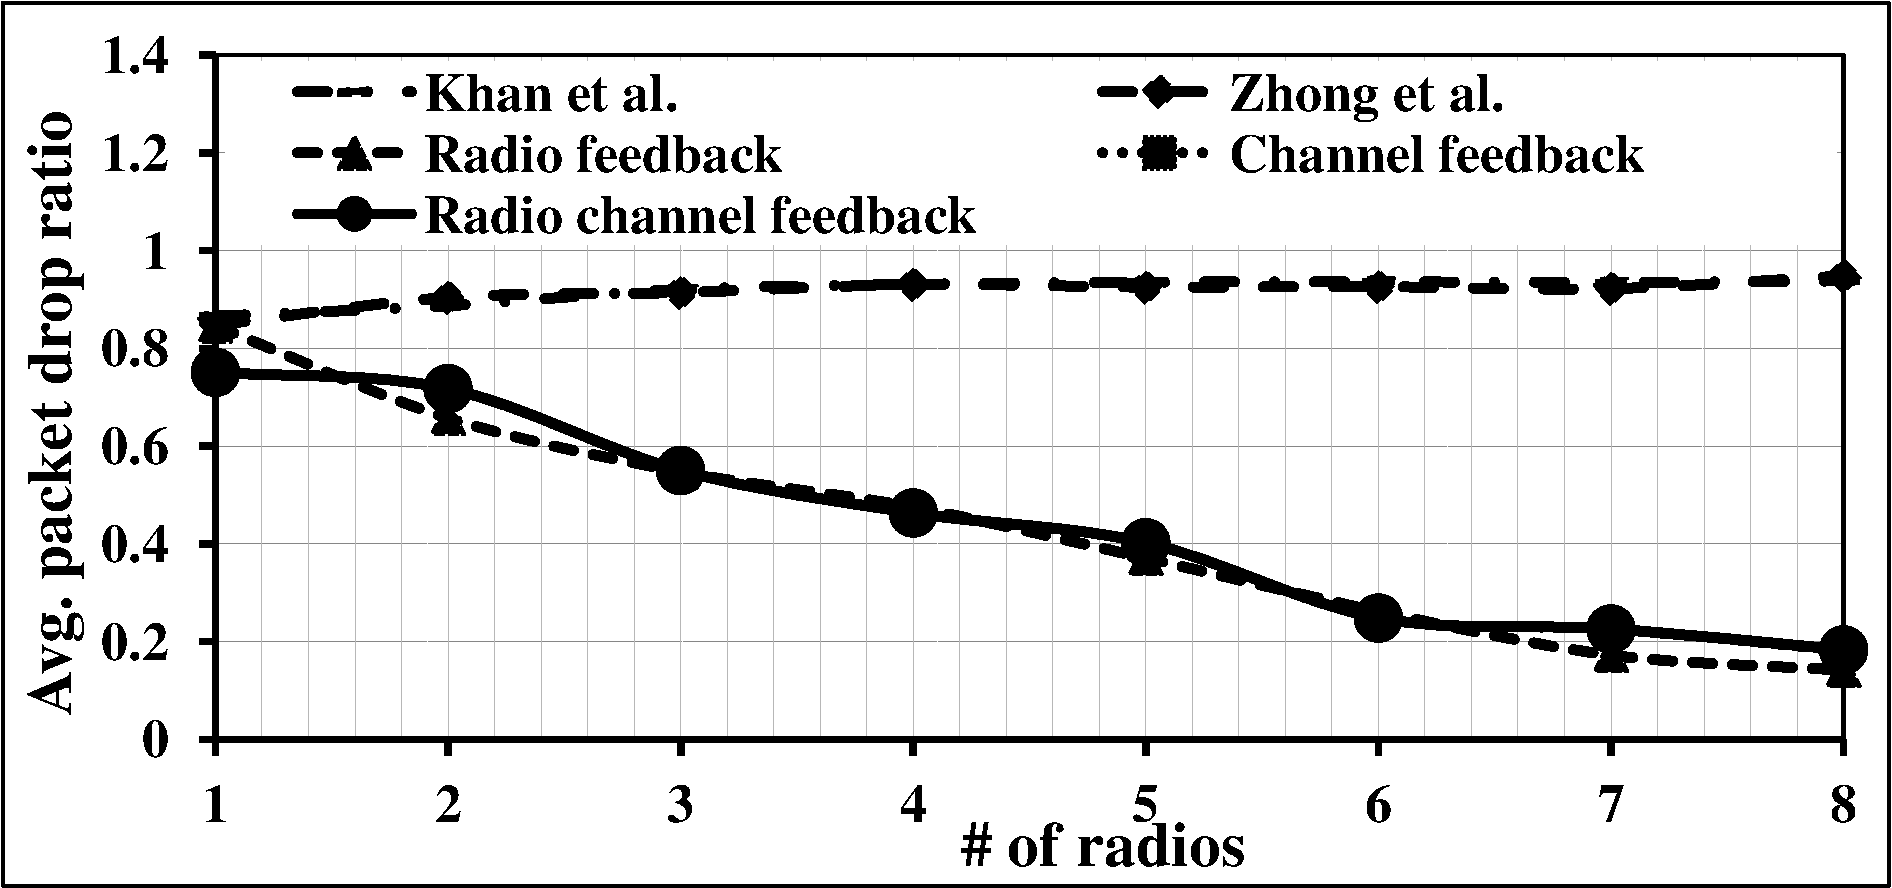
\includegraphics[width=\textwidth]{topology4/PacketDropRatio24d2}
        \caption{2Mbps application data rate}
        \label{fig:topology4P2}
    \end{subfigure}
    ~\\
    \begin{subfigure}[t]{0.625\textwidth}
        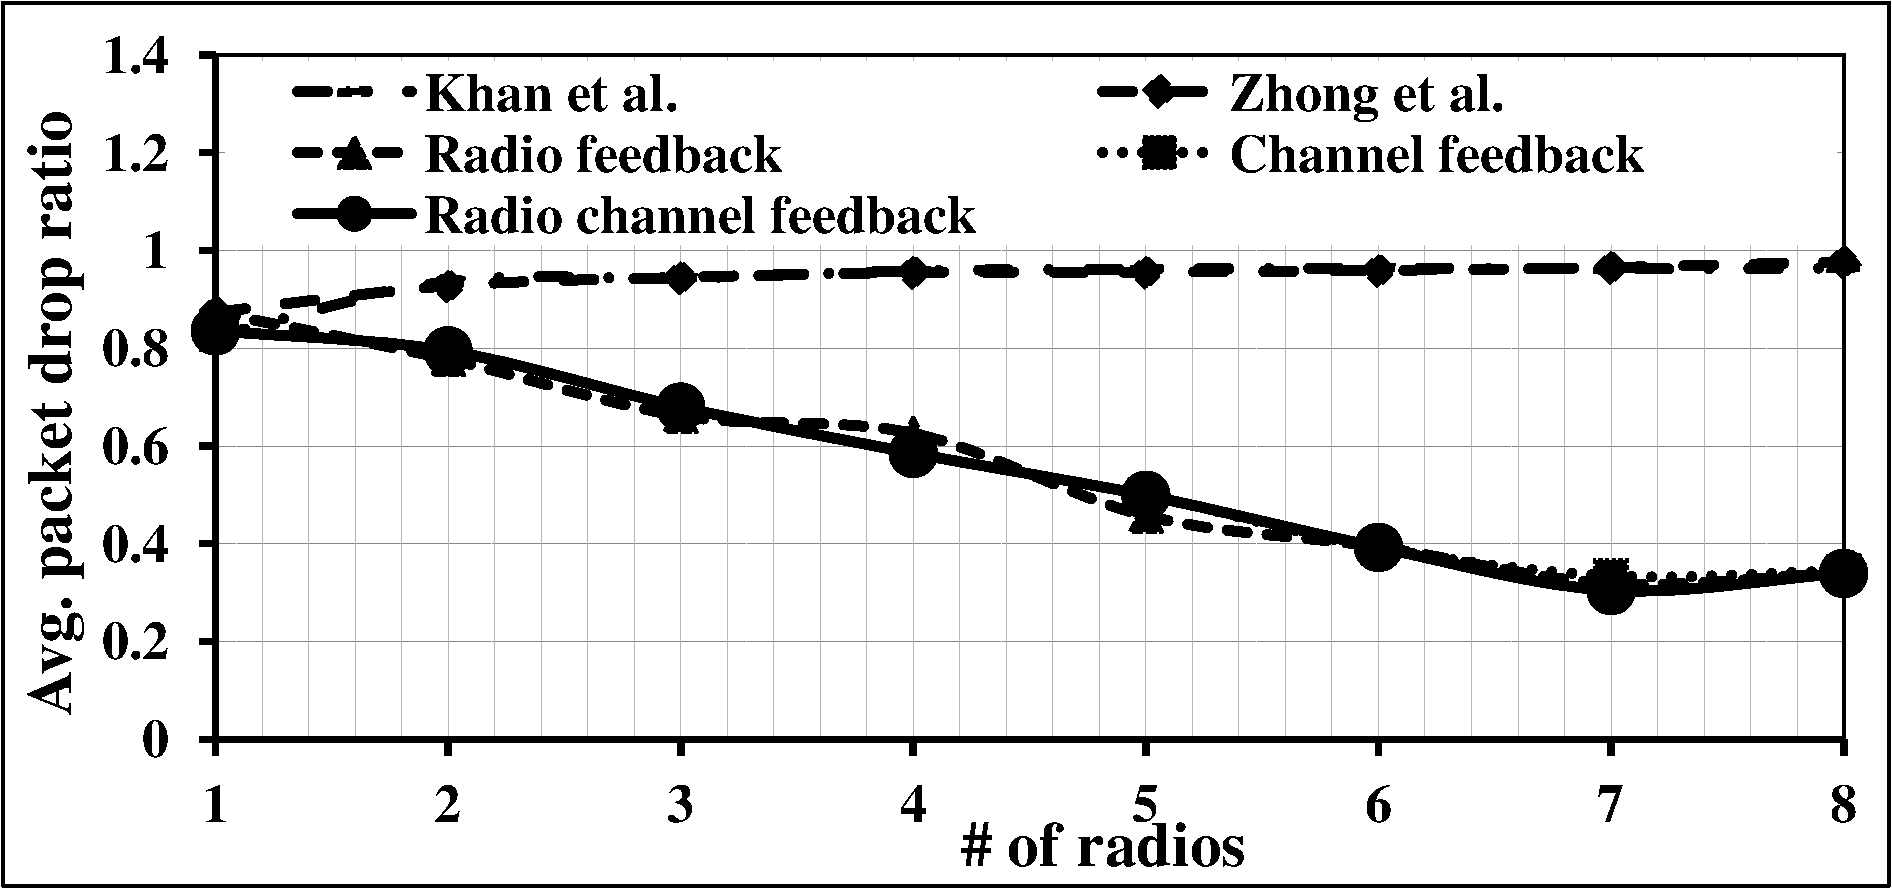
\includegraphics[width=\textwidth]{topology4/PacketDropRatio24d4}
        \caption{4Mbps application data rate}
        \label{fig:topology4P3}
    \end{subfigure}
    ~
    \begin{subfigure}[t]{0.625\textwidth}
        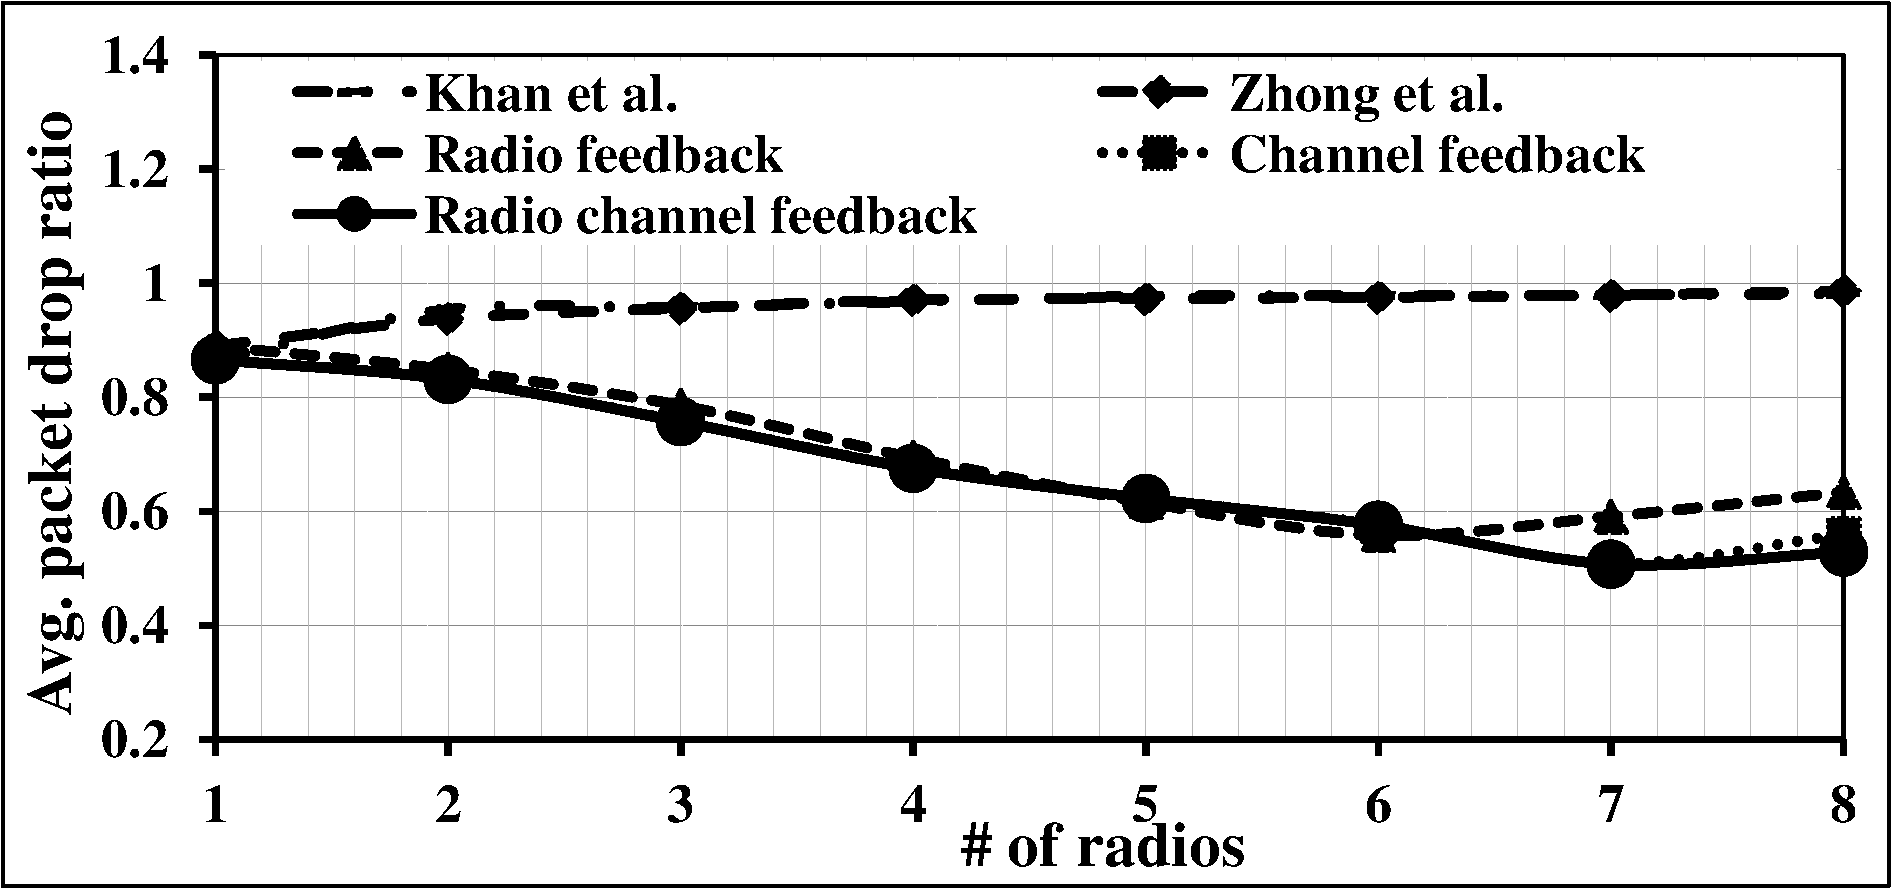
\includegraphics[width=\textwidth]{topology4/PacketDropRatio24d8}
        \caption{8Mbps application data rate}
        \label{fig:topology4P4}
    \end{subfigure}
    ~\\
    \begin{subfigure}[t]{0.625\textwidth}
        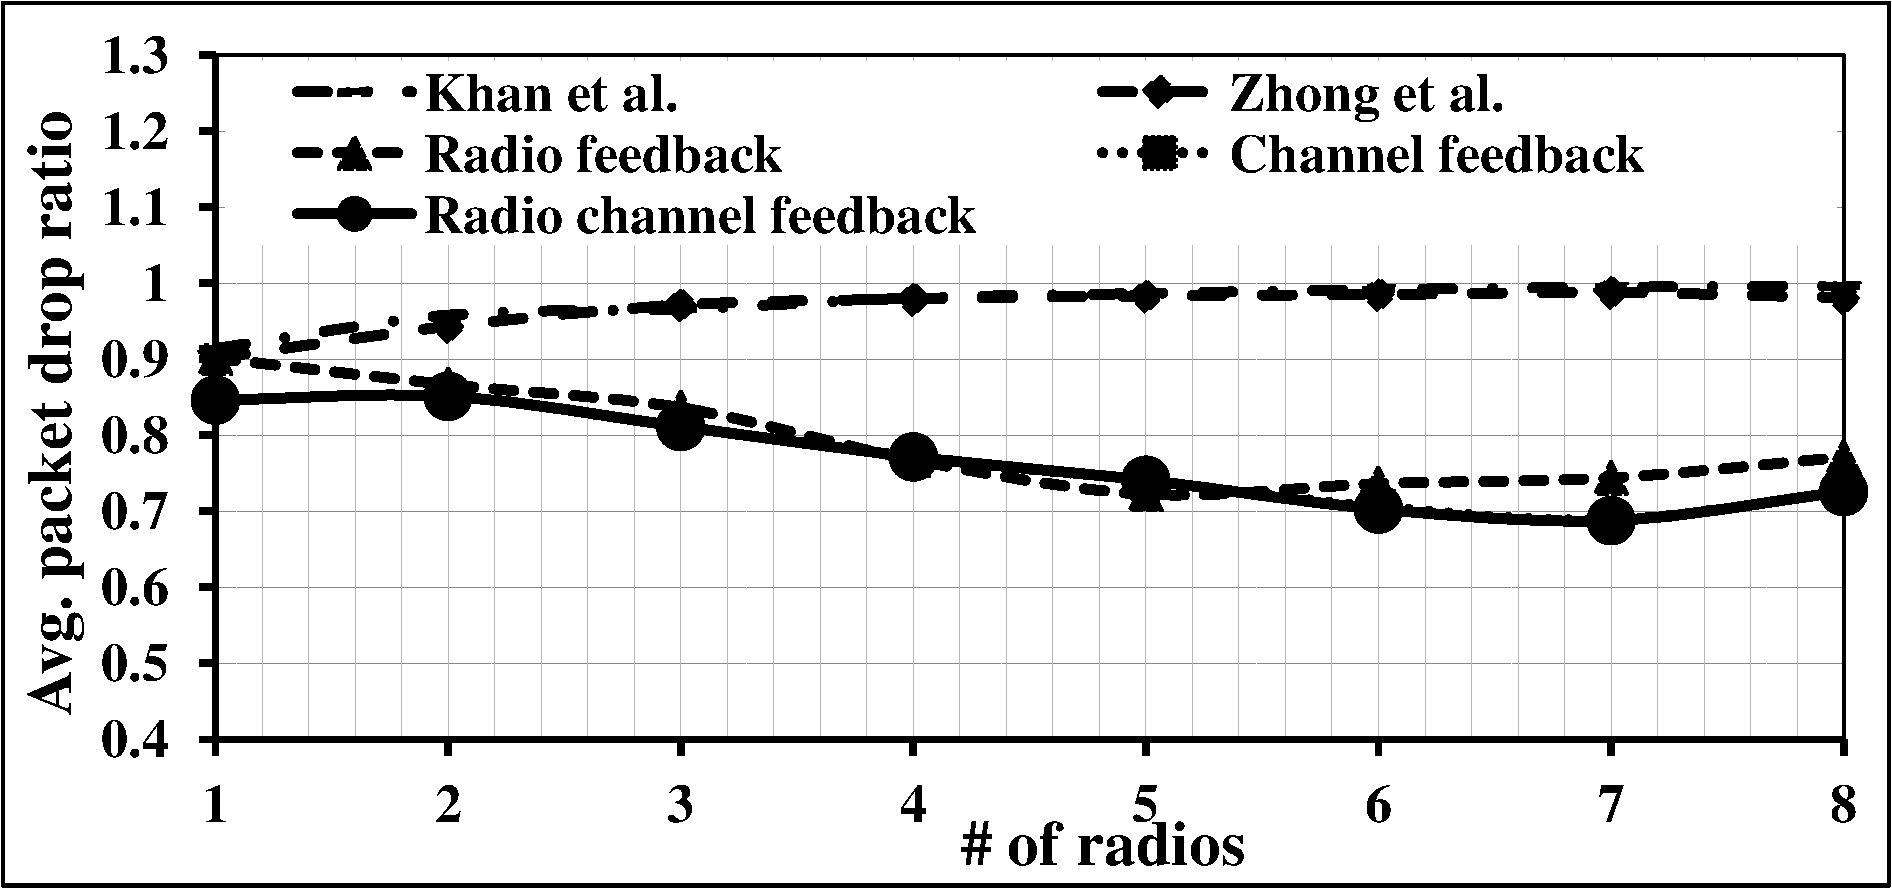
\includegraphics[width=\textwidth]{topology4/PacketDropRatio24d16}
        \caption{16Mbps application data rate}
        \label{fig:topology4P5}
    \end{subfigure}
    ~
    \begin{subfigure}[t]{0.625\textwidth}
        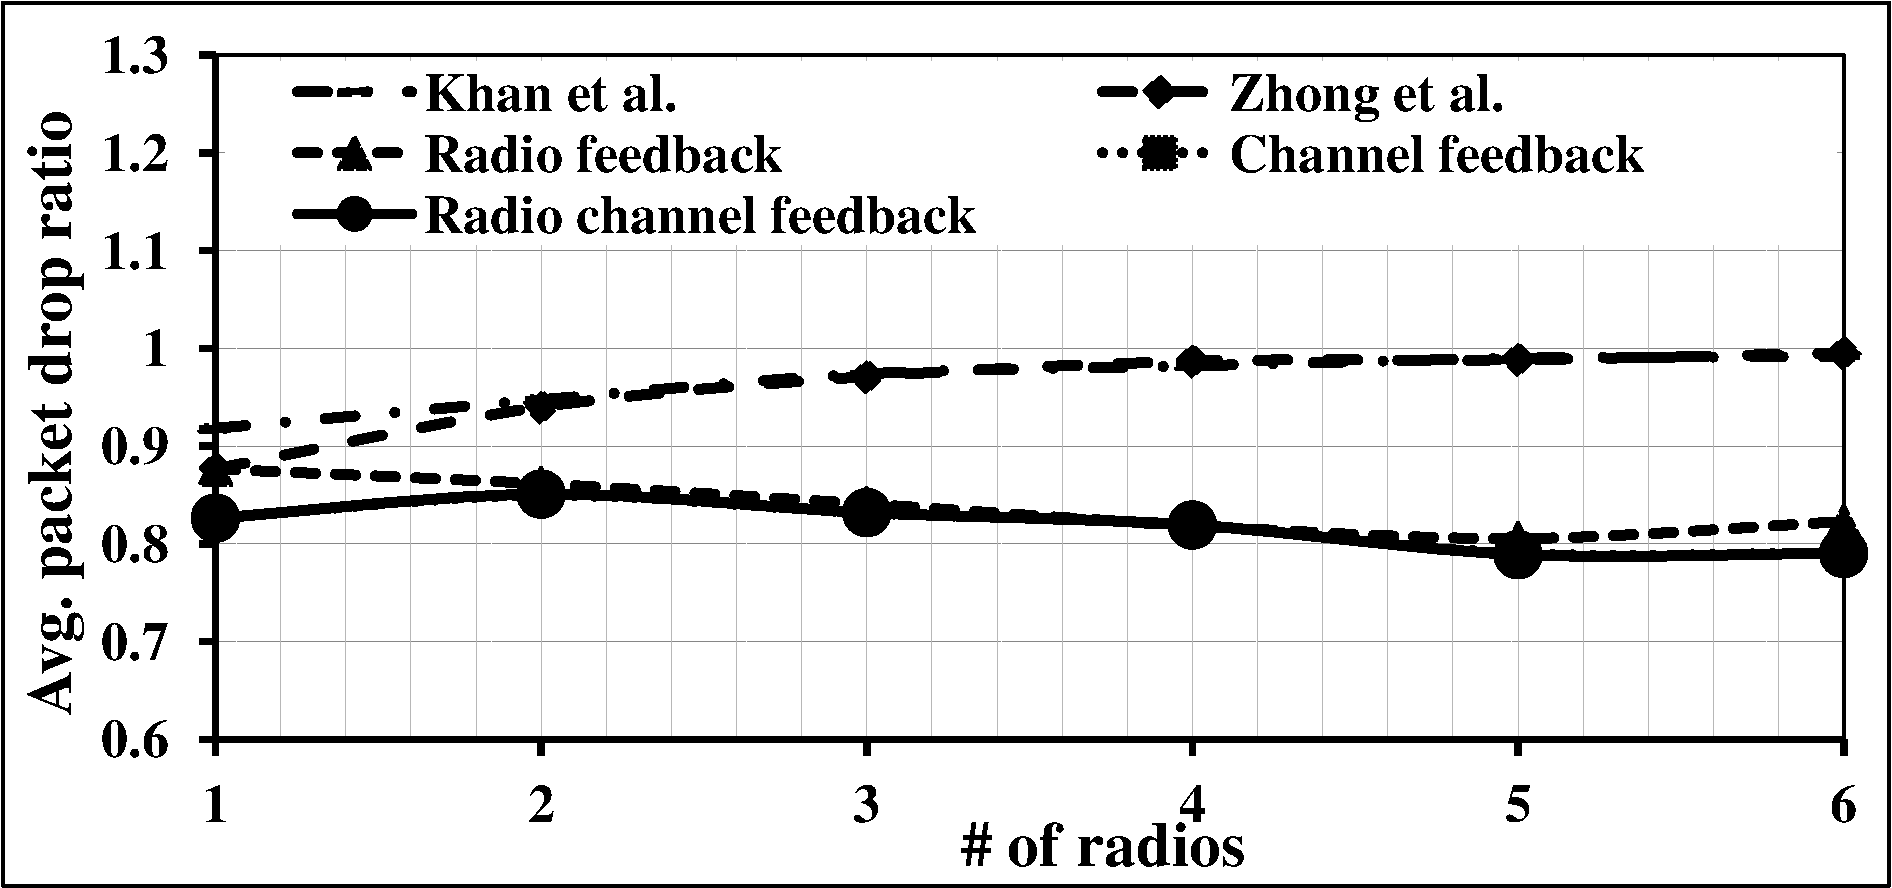
\includegraphics[width=\textwidth]{topology4/PacketDropRatio24d32}
        \caption{32Mbps application data rate}
        \label{fig:topology4P6}
    \end{subfigure}
    \caption{Average packet drop ratio with varying number of radios for various application data rates}
    \label{fig:topology4P}
\end{figure*}
\end{landscape}

\begin{figure*}[!htbp]
    \centering
    \begin{subfigure}[t]{0.45\textwidth}
        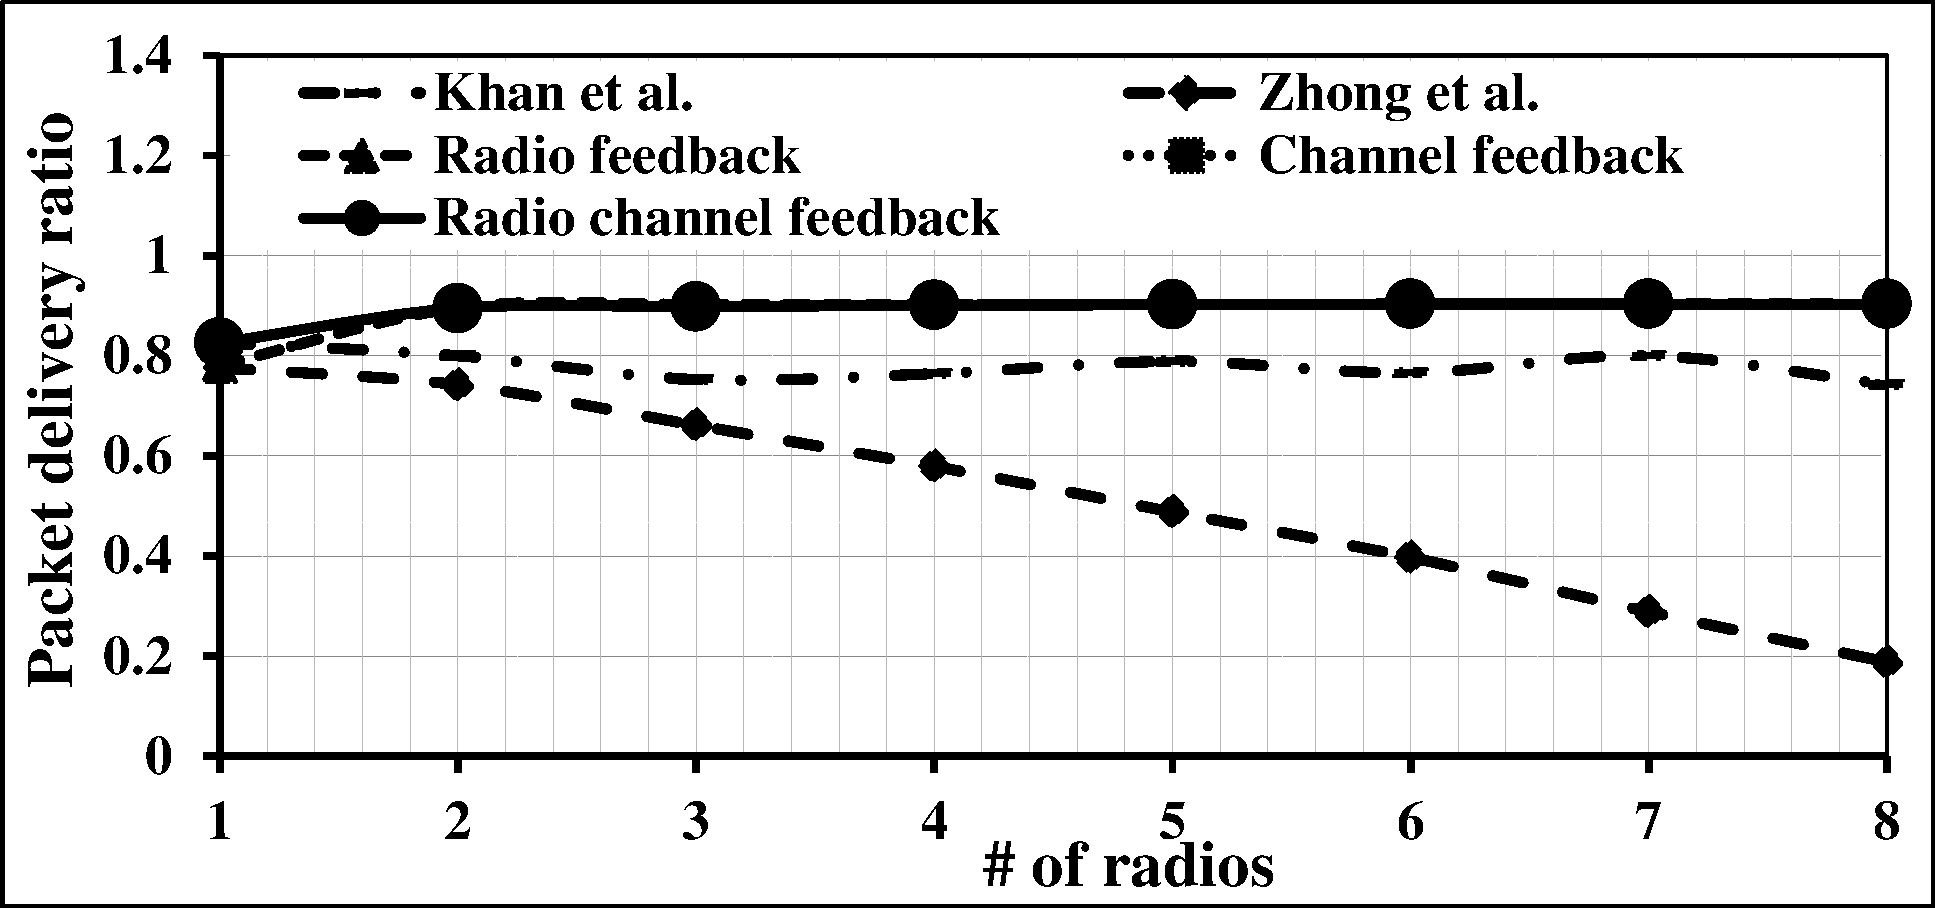
\includegraphics[width=\textwidth]{topology4/DeliveryRatio24d1}
        \caption{1Mbps application data rate}
        \label{fig:topology4PD1}
    \end{subfigure}
    ~
    \begin{subfigure}[t]{0.45\textwidth}
        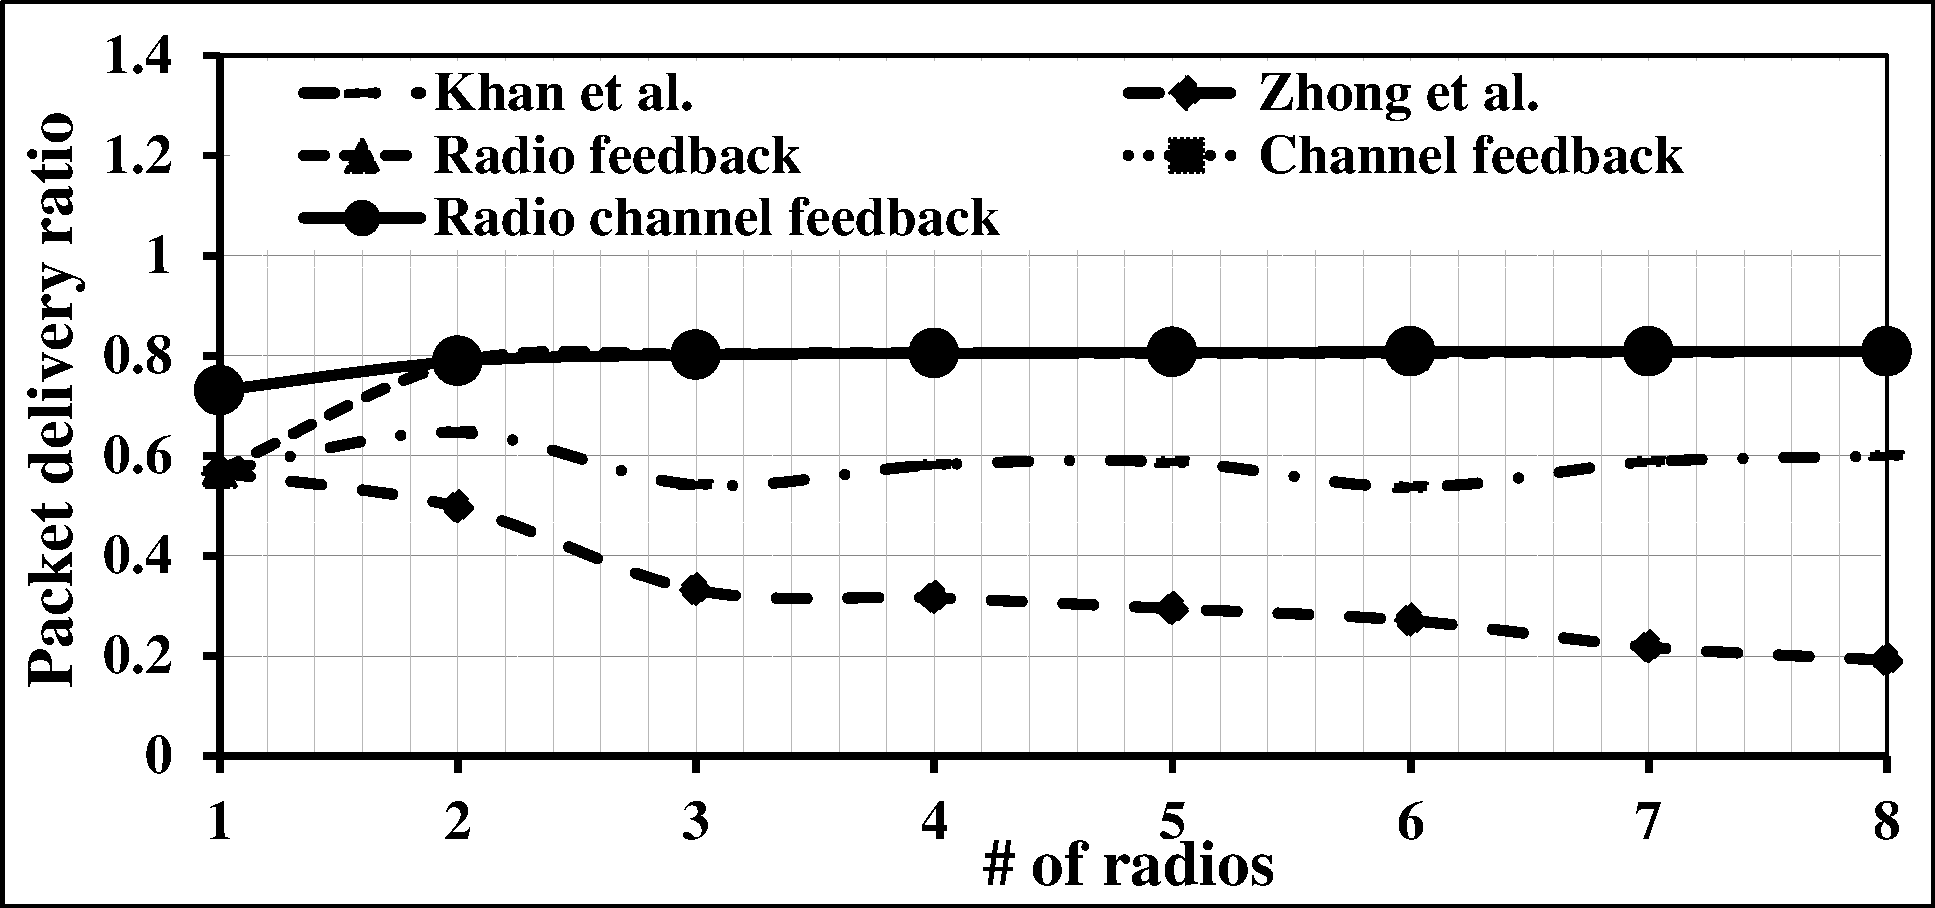
\includegraphics[width=\textwidth]{topology4/DeliveryRatio24d2}
        \caption{2Mbps application data rate}
        \label{fig:topology4PD2}
    \end{subfigure}
    ~\\
    \begin{subfigure}[t]{0.45\textwidth}
        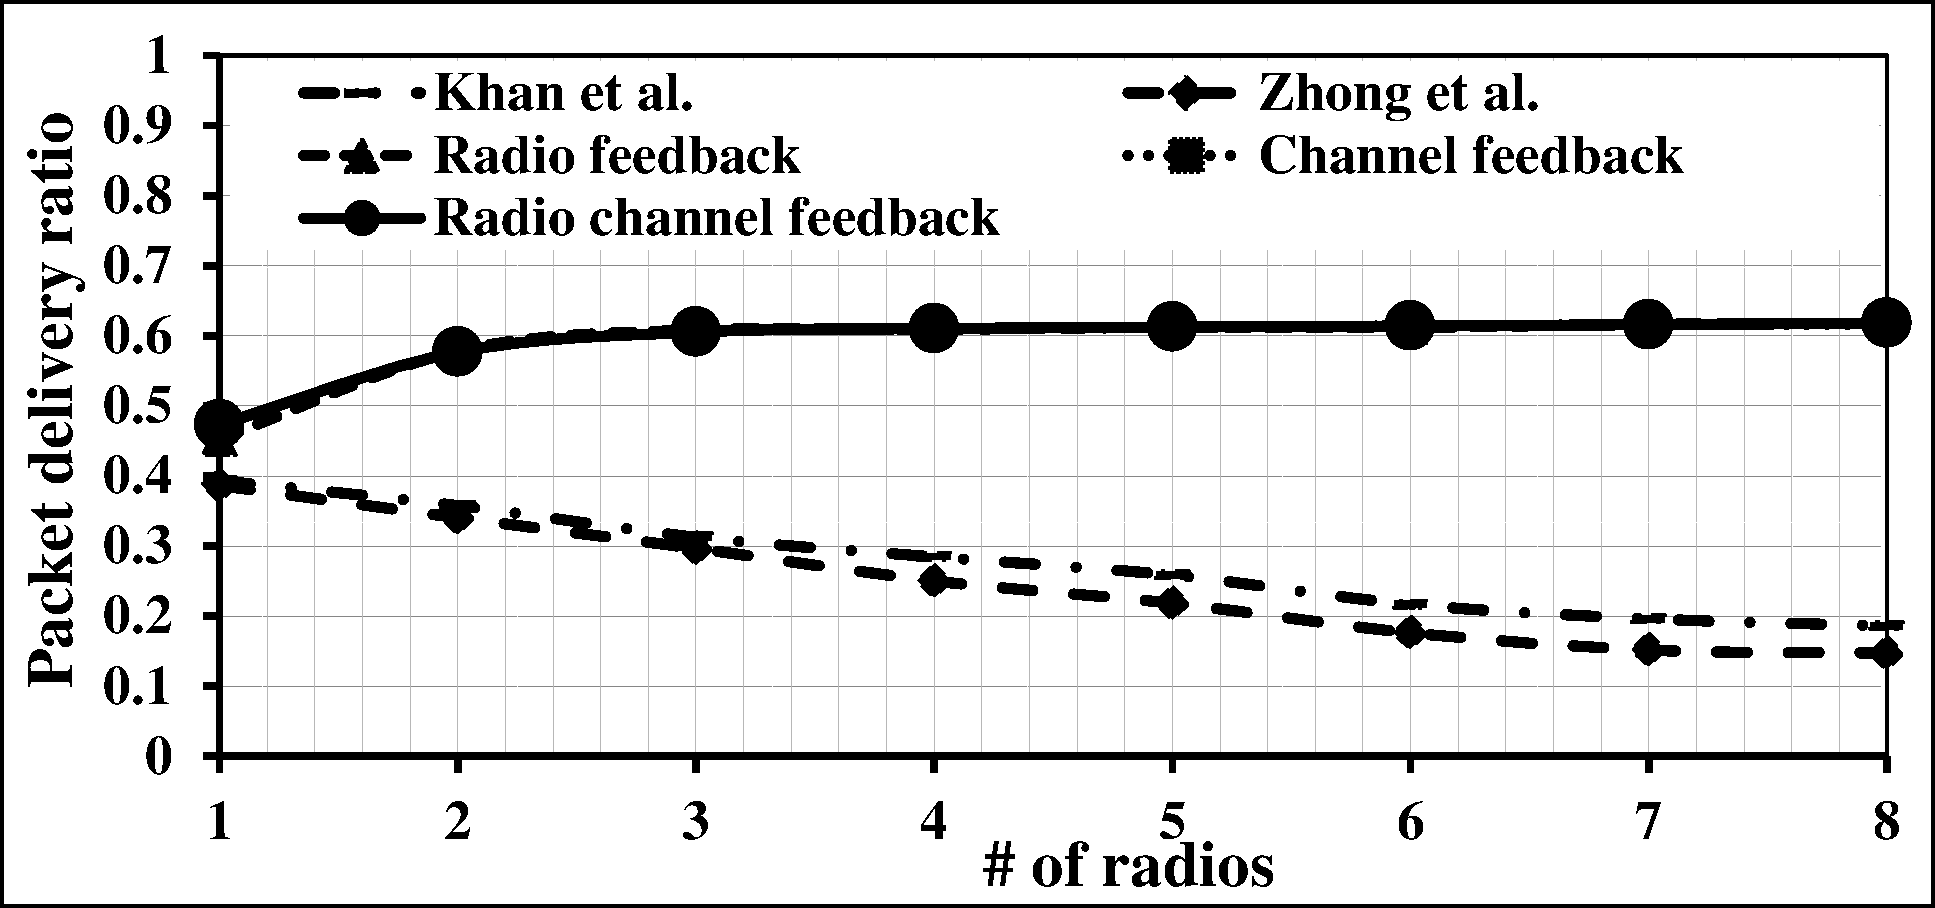
\includegraphics[width=\textwidth]{topology4/DeliveryRatio24d4}
        \caption{4Mbps application data rate}
        \label{fig:topology4PD3}
    \end{subfigure}
    ~
    \begin{subfigure}[t]{0.45\textwidth}
        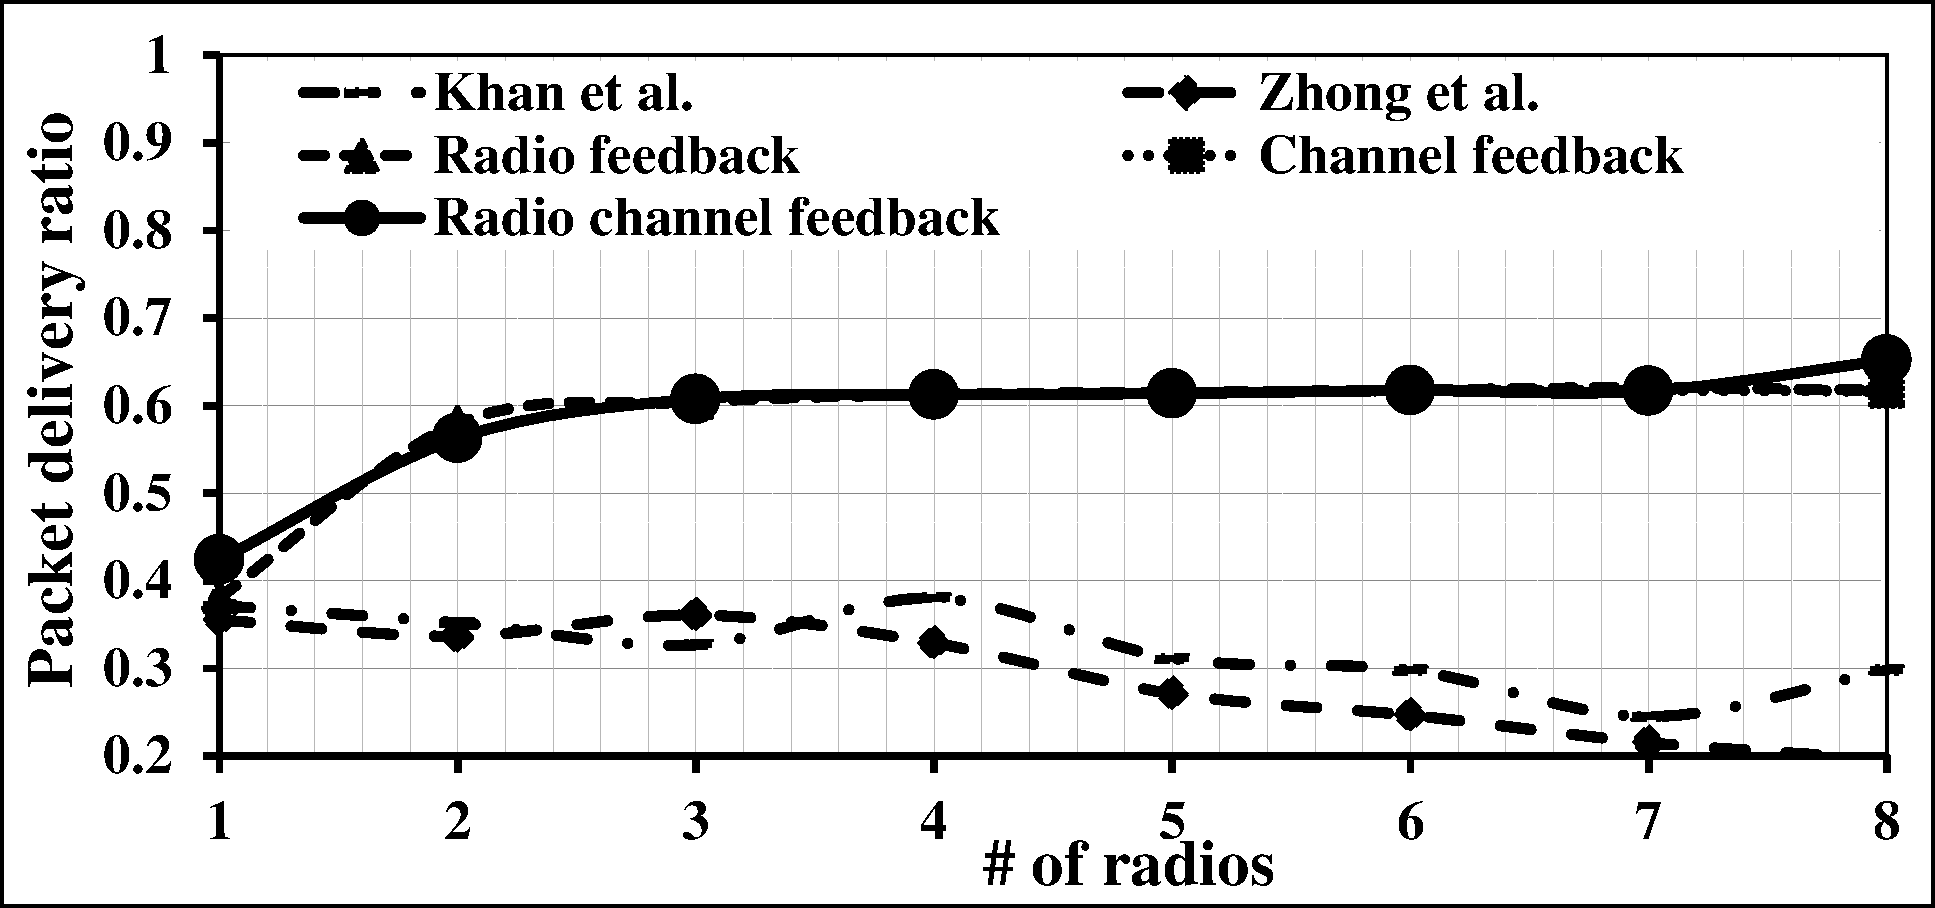
\includegraphics[width=\textwidth]{topology4/DeliveryRatio24d8}
        \caption{8Mbps application data rate}
        \label{fig:topology4PD4}
    \end{subfigure}
    ~\\
    \begin{subfigure}[t]{0.45\textwidth}
        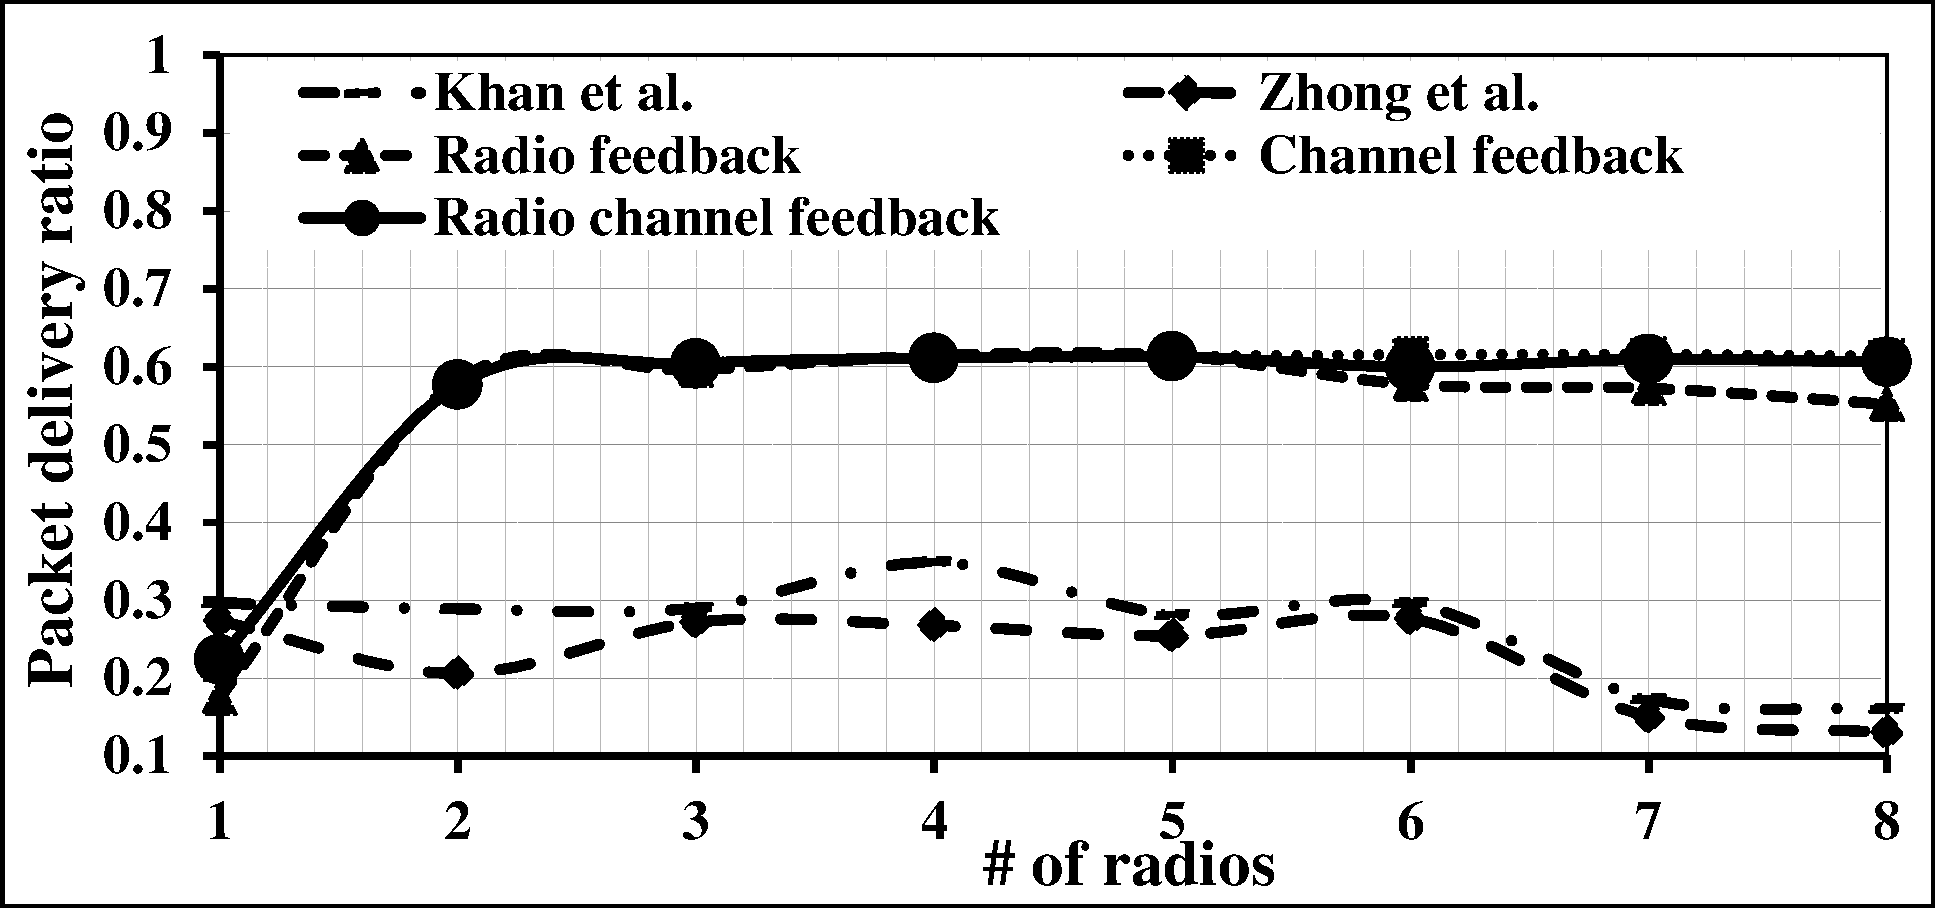
\includegraphics[width=\textwidth]{topology4/DeliveryRatio24d16}
        \caption{16Mbps application data rate}
        \label{fig:topology4PD5}
    \end{subfigure}
    ~
    \begin{subfigure}[t]{0.45\textwidth}
        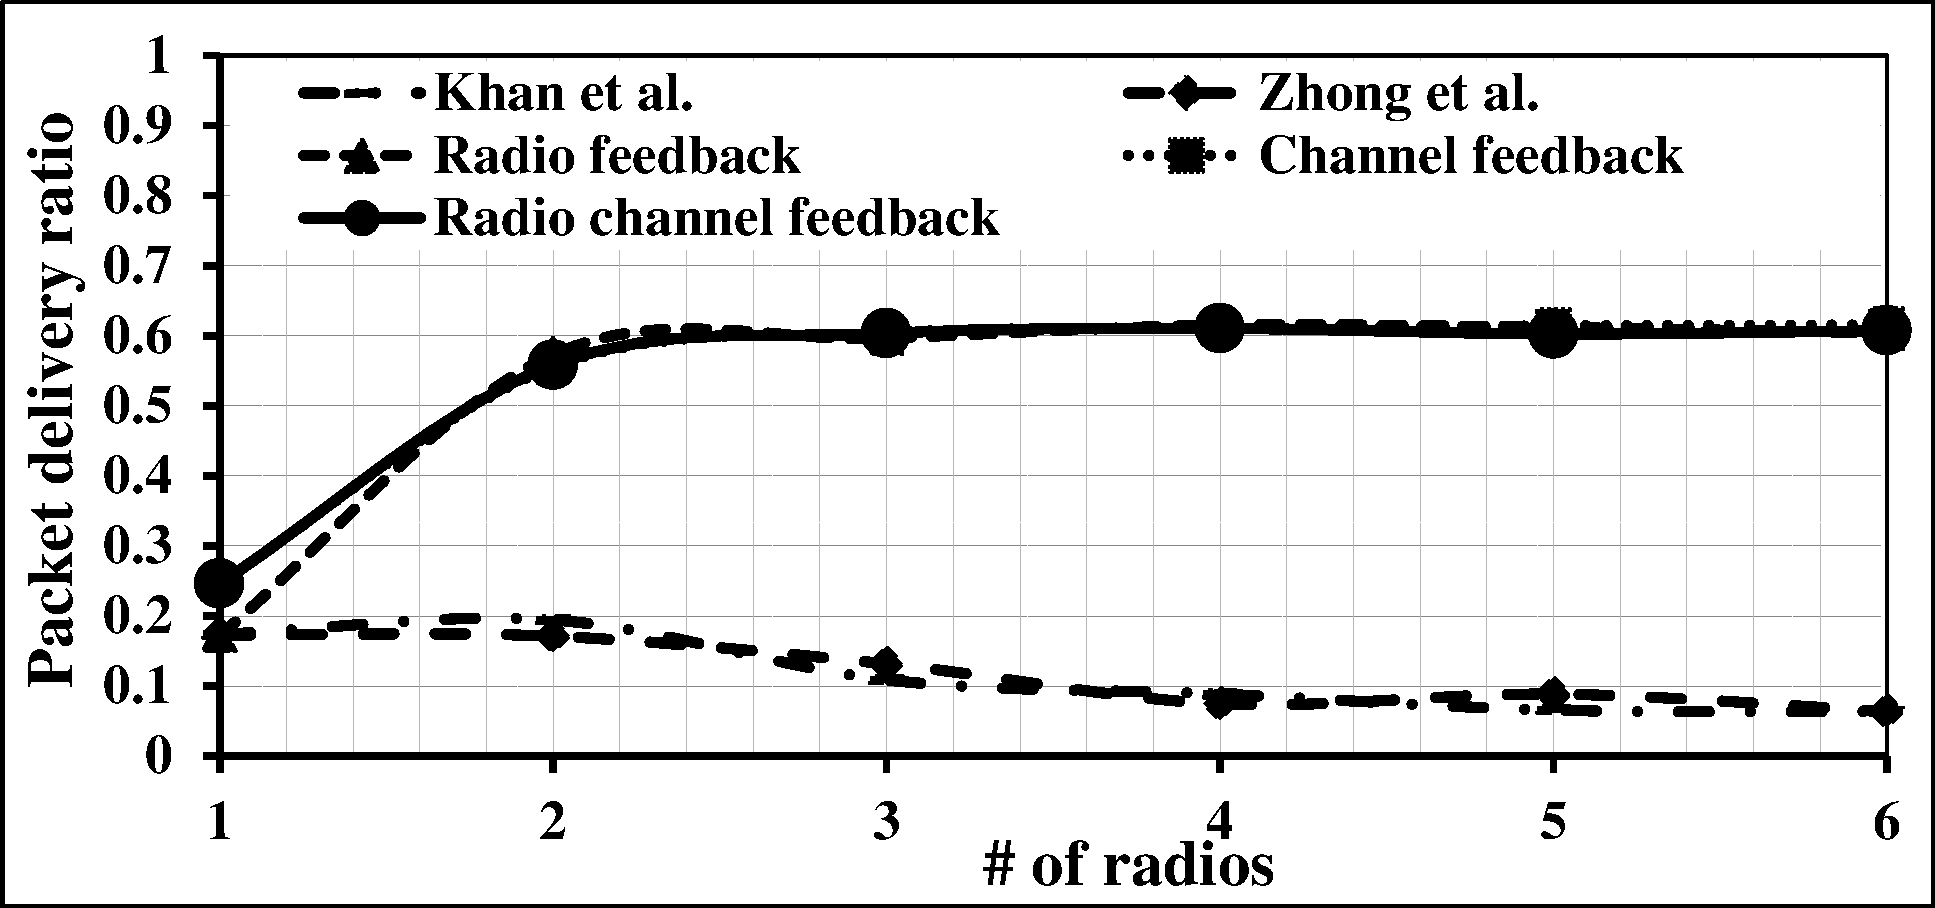
\includegraphics[width=\textwidth]{topology4/DeliveryRatio24d32}
        \caption{32Mbps application data rate}
        \label{fig:topology4PD6}
    \end{subfigure}
    \caption{Application layer packet delivery ratio with varying number of radios for various application data rates}
    \label{fig:topology4PD}
\end{figure*}


Fig.~\ref{fig:topology4T} depicts total network throughput for all the approaches in response to a variation in the number of radios for different application data rates. In most of the cases, our proposed approaches obtain significantly higher network throughput than the existing ones. Here, at lower data rates (1-8 Mbps), total network throughput increases with an increase in the number of radios. After reaching an optimal point, throughput starts degrading. At higher data rates (16 and 32 Mbps), the network throughput falls drastically from the single radio scenario and never again reaches the throughput obtained with single radio data transmission.

Fig.~\ref{fig:topology4D} illustrates that the feedback-based approaches experience significantly lower end-to-end delay than that achieved with the approach proposed by Zhong et al.~\cite{zhong2014capacity}. However, delay using our proposed approach is higher than that achieved with the approach proposed by Khan et al.~\cite{khan2015towards}. Here with our proposed approach, the delay becomes almost constant with an increase in the number of radios at lower application date rates (1-4Mbps). However, at higher data rates (8-32 Mbps), the delay rises with an increase in the number of radios per SU.

Fig.~\ref{fig:topology4P} compares the average packet drop ratio of our proposed approaches against that of the existing approaches.  As illustrated in \cref{fig:topology4P}, the feedback-based approach achieves significantly lower packet drop ratios than all the existing ones. The feedback-based approach is also able to reduce the packet drop ratio significantly at lower data rates (1-8 Mbps) with the exploitation of multiple radios. However, at higher application data rates (16 and 32 Mbps), most of the packets get dropped resulting in high drop ratios. This explains why the network throughput at higher data rate does not improve even after the introduction of multiple data transmission radios.

Fig.~\ref{fig:topology4PD} shows the application layer packet delivery ratio of our proposed approaches against that of the existing approaches. Due to the efficient exploitation of multiple radios, our proposed approaches obtain significantly better packet delivery ratio than that achieved with the existing appraoches.

Table~\ref{tab:topology4RadioImprovement}, \ref{tab:topology4ChannelImprovement}, and \ref{tab:topology4RadioChannelImprovement} summarize average performance improvement using feedback-based approaches in comparison to the approaches proposed by Khan et al.,~\cite{khan2015towards} and Zhong et al.~\cite{zhong2014capacity}. The tables shows that the proposed approach outperforms the existing approaches in terms of all the performance metrics except end-to-end delay. In terms of total network throughput, the proposed approach obtains an average of 51\% improvement over the two existing approaches. Moreover, the proposed approach decreases packet drop ratio on an average 35\% and increases application layer packet delivery ratio on an average 32\% compared to existing approaches. Even though, the feedback-based approach experiences the higher delay in some cases, in average, the delay is improved by 13\% on an average.
%\begin{figure*}[!htbp]
    \centering
    \begin{subfigure}[t]{0.45\textwidth}
        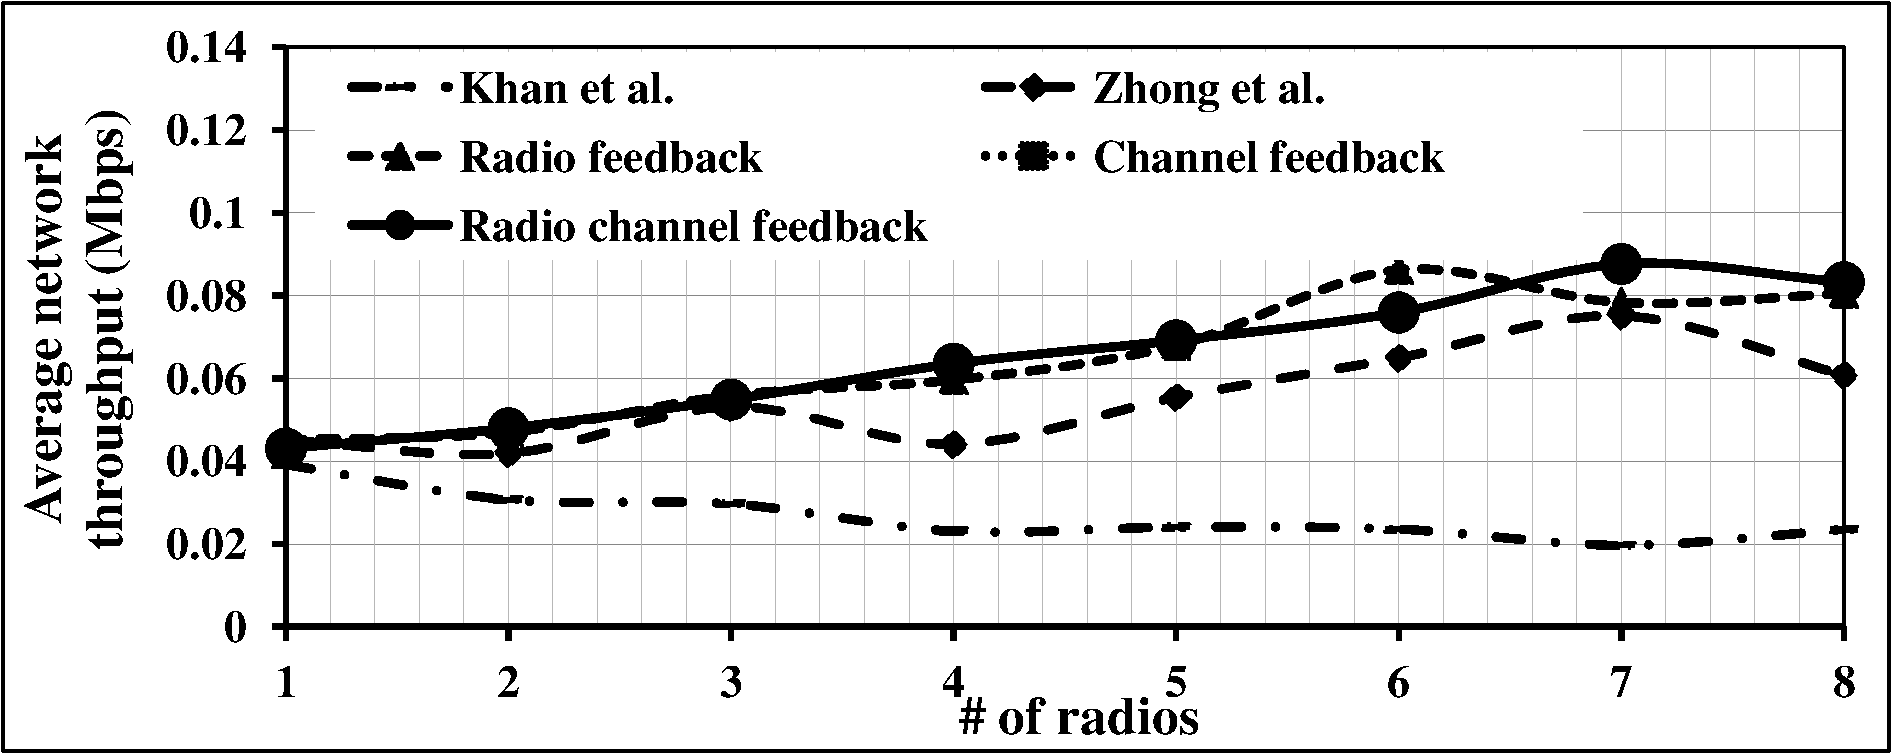
\includegraphics[width=\textwidth]{topology4/Throughput24d1}
        \caption{1Mbps application data rate}
        \label{fig:topology4T1}
    \end{subfigure}
    ~
    \begin{subfigure}[t]{0.45\textwidth}
        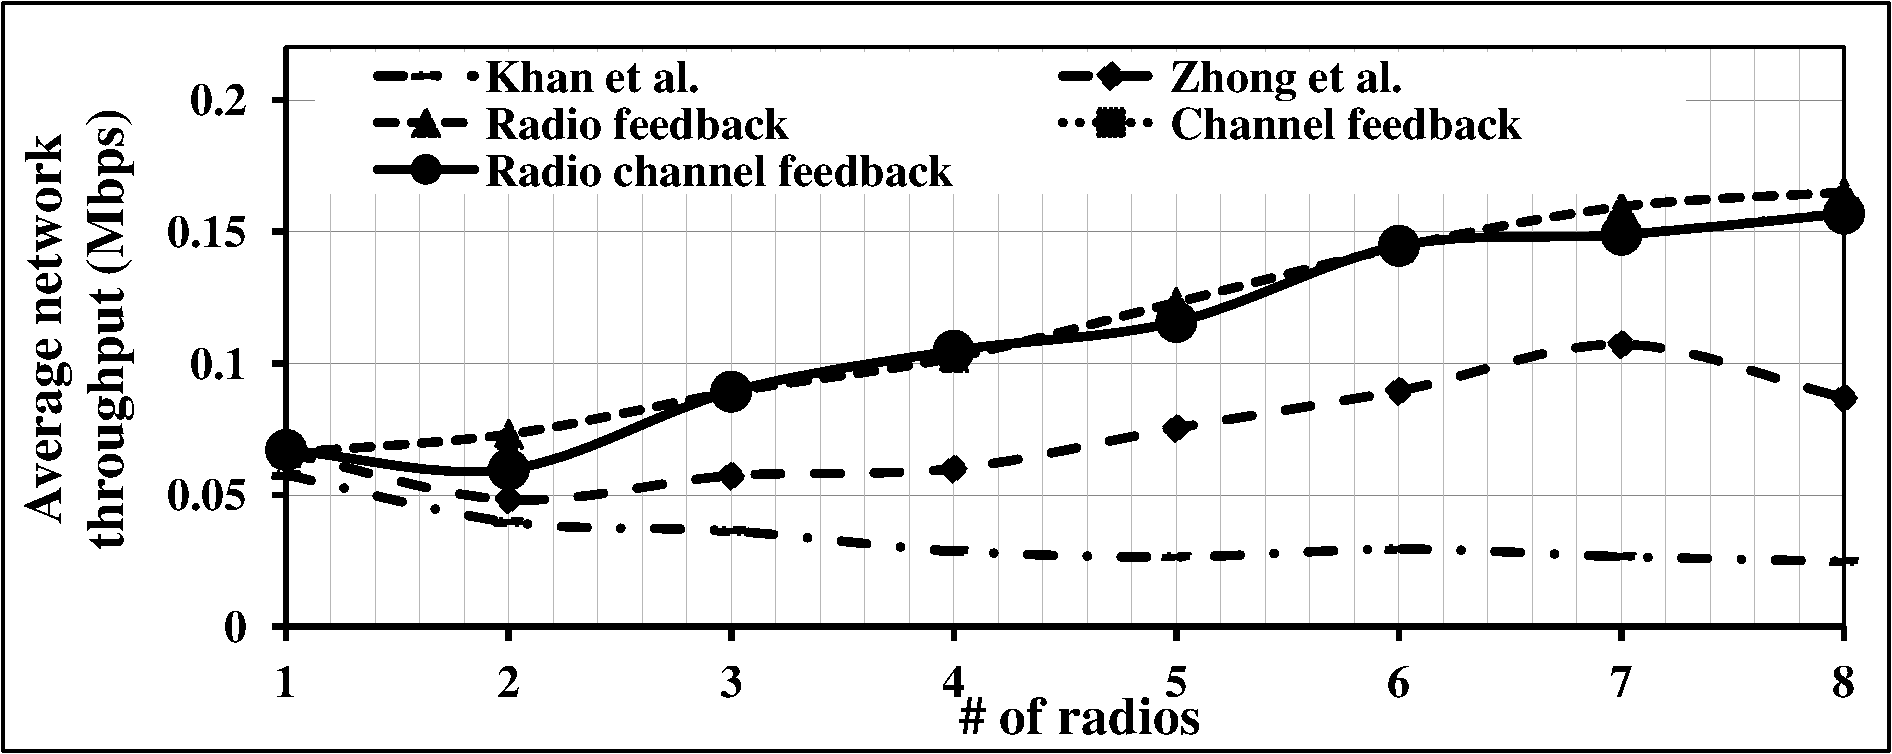
\includegraphics[width=\textwidth]{topology4/Throughput24d2}
        \caption{2Mbps application data rate}
        \label{fig:topology4T2}
    \end{subfigure}
    ~\\
    \begin{subfigure}[t]{0.45\textwidth}
        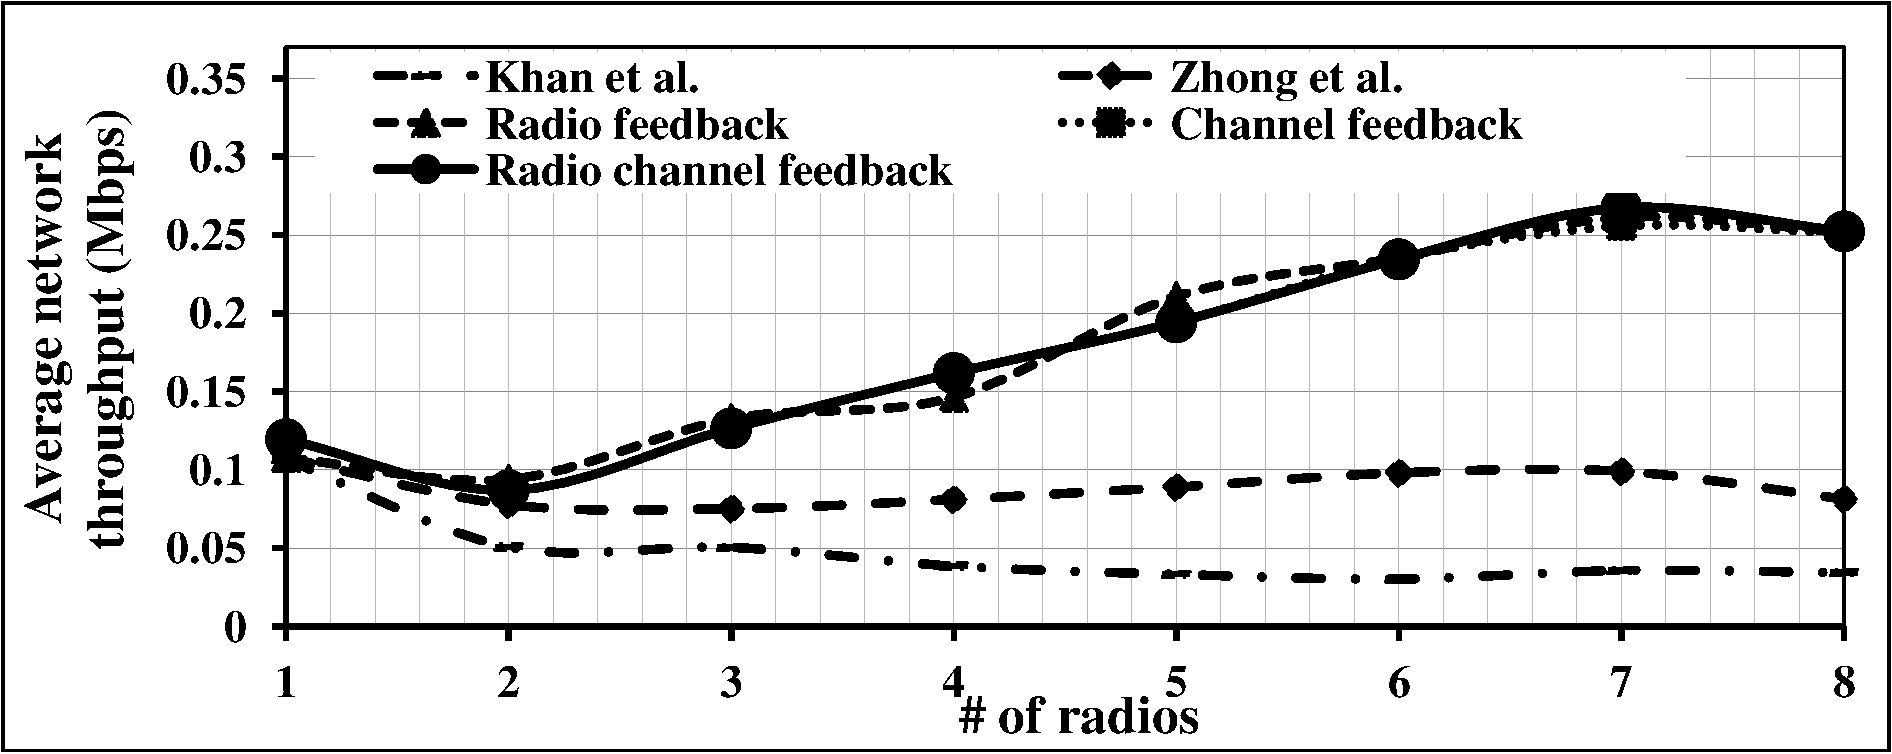
\includegraphics[width=\textwidth]{topology4/Throughput24d4}
        \caption{4Mbps application data rate}
        \label{fig:topology4T3}
    \end{subfigure}
    ~
    \begin{subfigure}[t]{0.45\textwidth}
        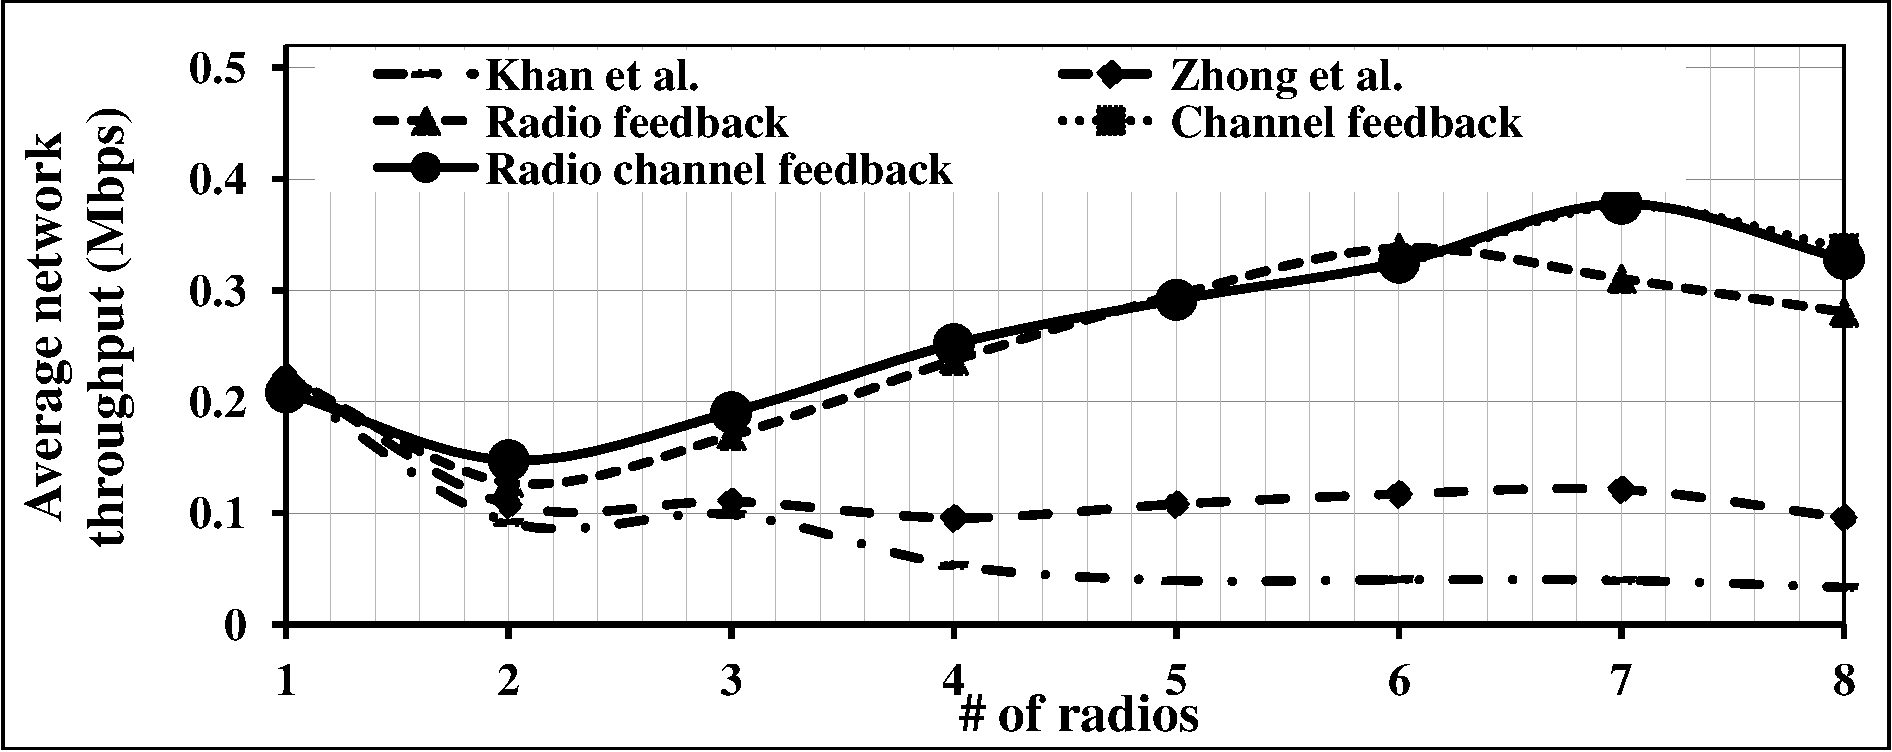
\includegraphics[width=\textwidth]{topology4/Throughput24d8}
        \caption{8Mbps application data rate}
        \label{fig:topology4T4}
    \end{subfigure}
    ~\\
    \begin{subfigure}[t]{0.45\textwidth}
        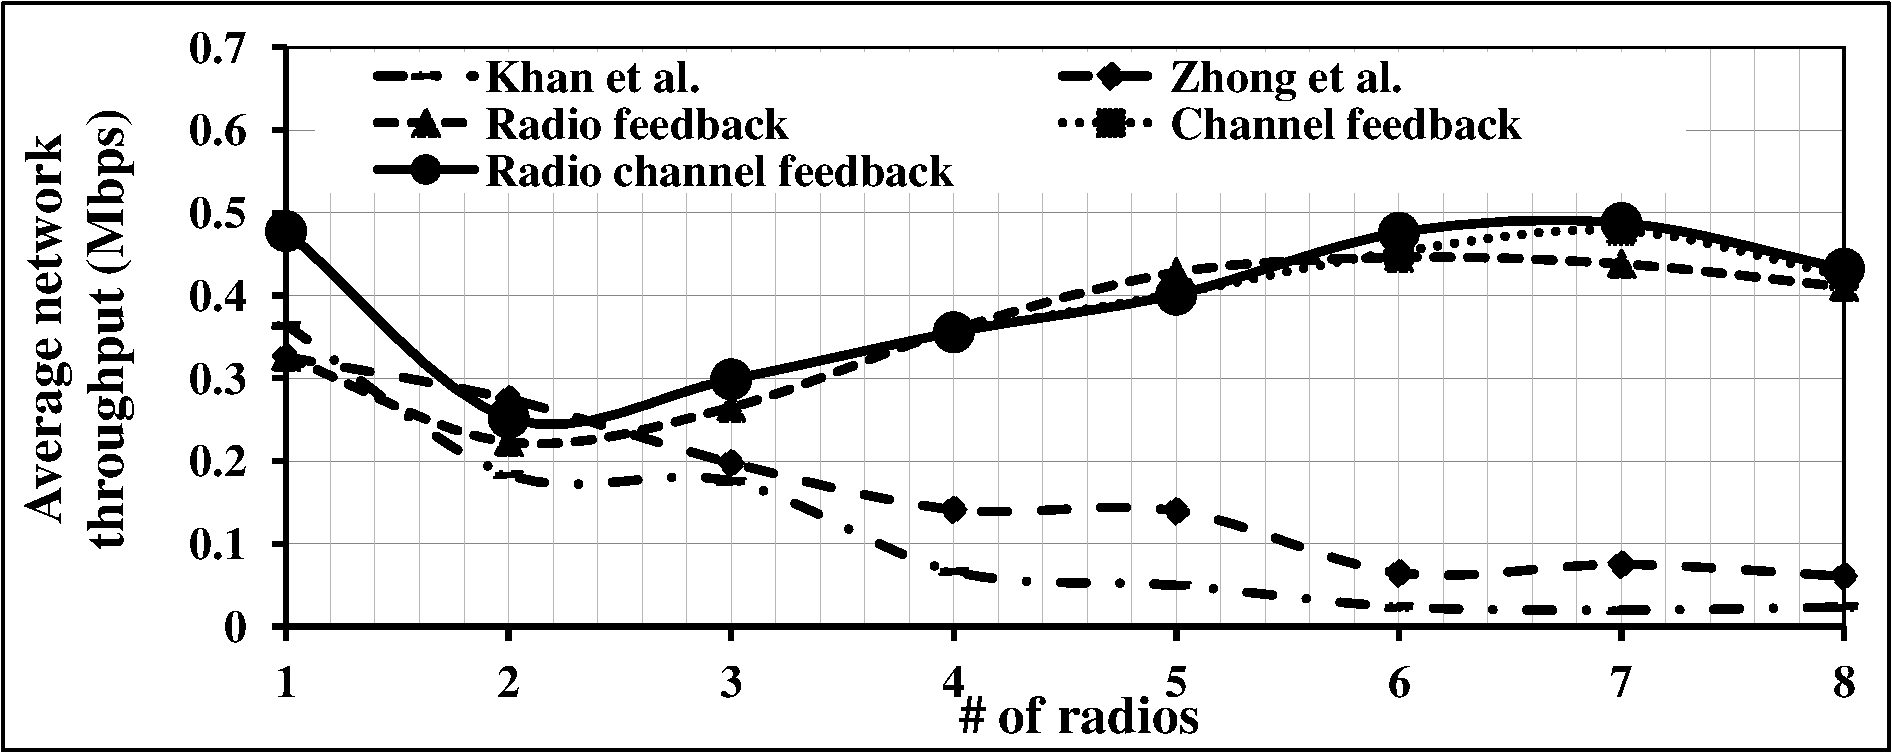
\includegraphics[width=\textwidth]{topology4/Throughput24d16}
        \caption{16Mbps application data rate}
        \label{fig:topology4T5}
    \end{subfigure}
    ~
    \begin{subfigure}[t]{0.45\textwidth}
        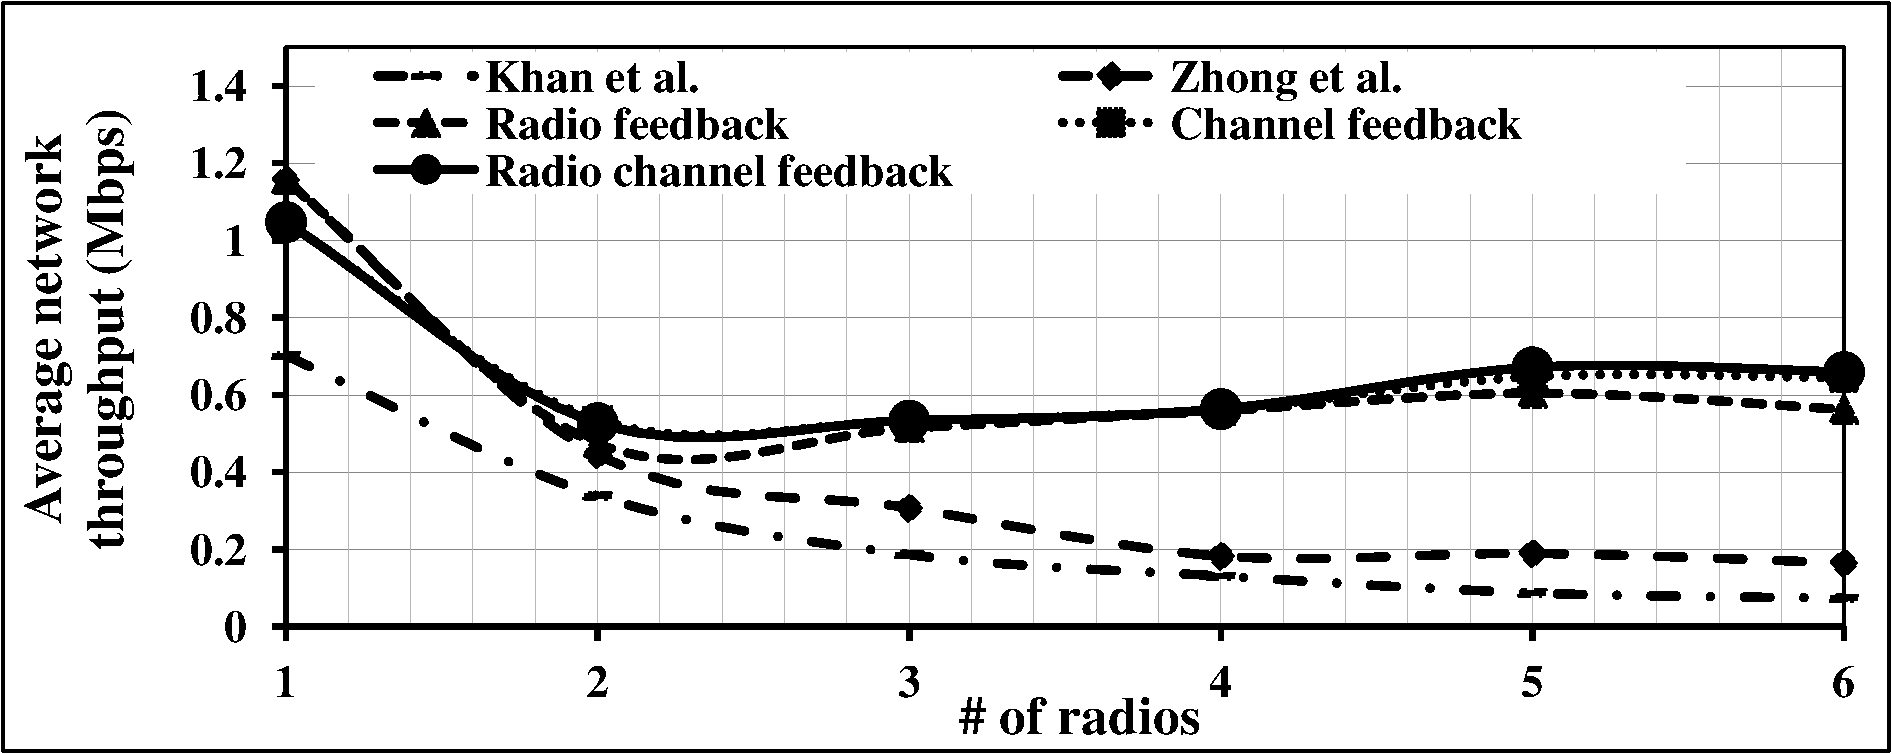
\includegraphics[width=\textwidth]{topology4/Throughput24d32}
        \caption{32Mbps application data rate}
        \label{fig:topology4T6}
    \end{subfigure}
    \caption{Average network throughput with varying number of radios for various application data rates}
    \label{fig:topology4T}
\end{figure*}

\begin{figure*}[!htbp]
    \centering
    \begin{subfigure}[t]{0.45\textwidth}
        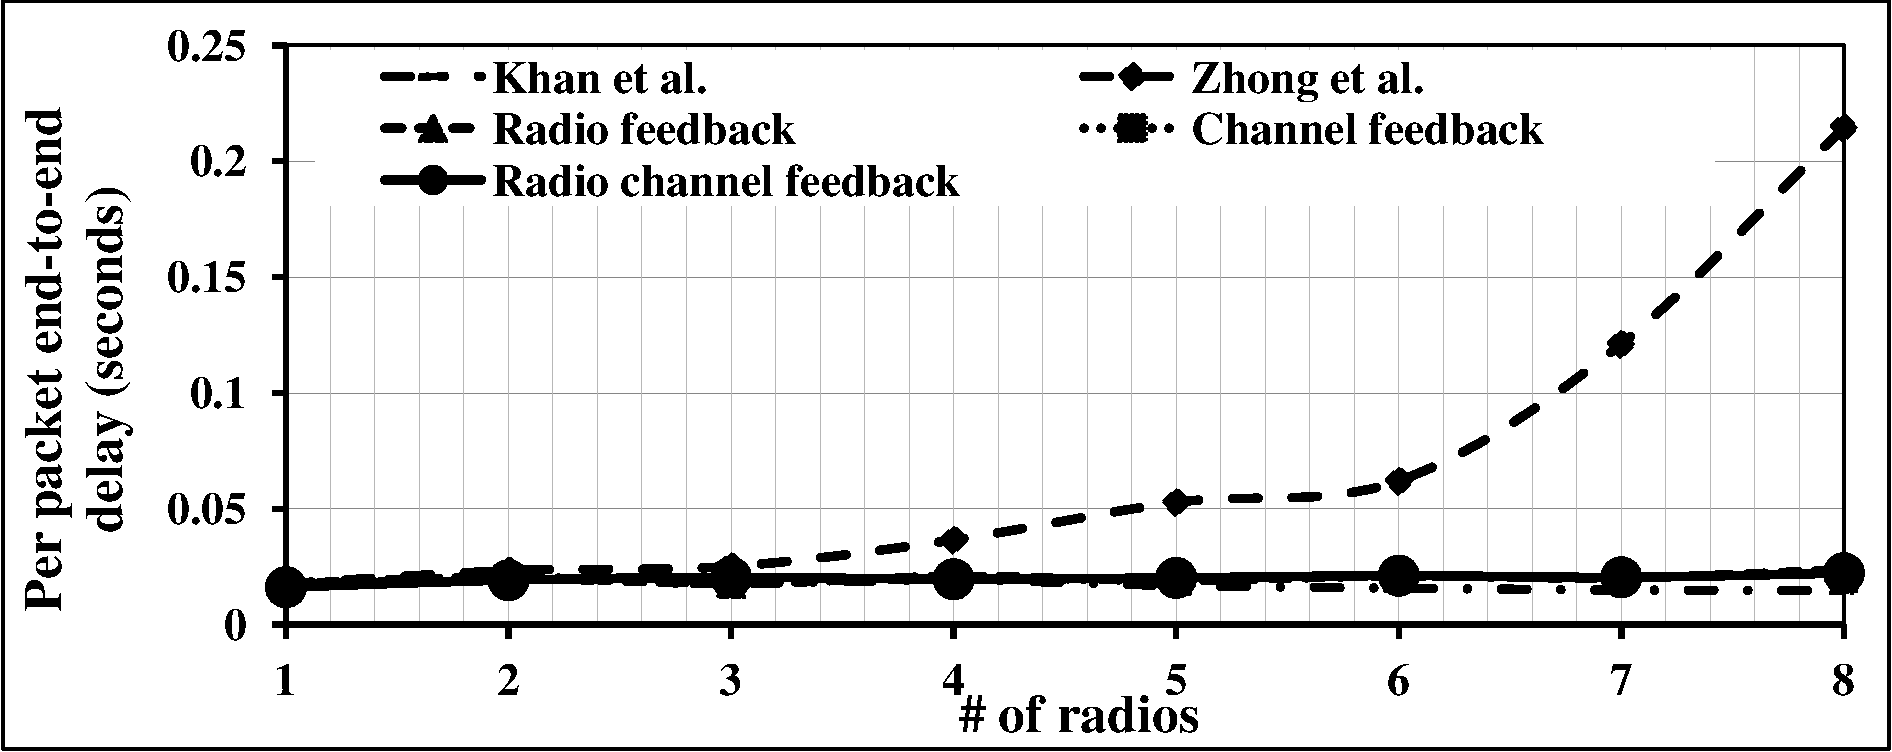
\includegraphics[width=\textwidth]{topology4/Delay24d1}
        \caption{1Mbps application data rate}
        \label{fig:topology4D1}
    \end{subfigure}
    ~
    \begin{subfigure}[t]{0.45\textwidth}
        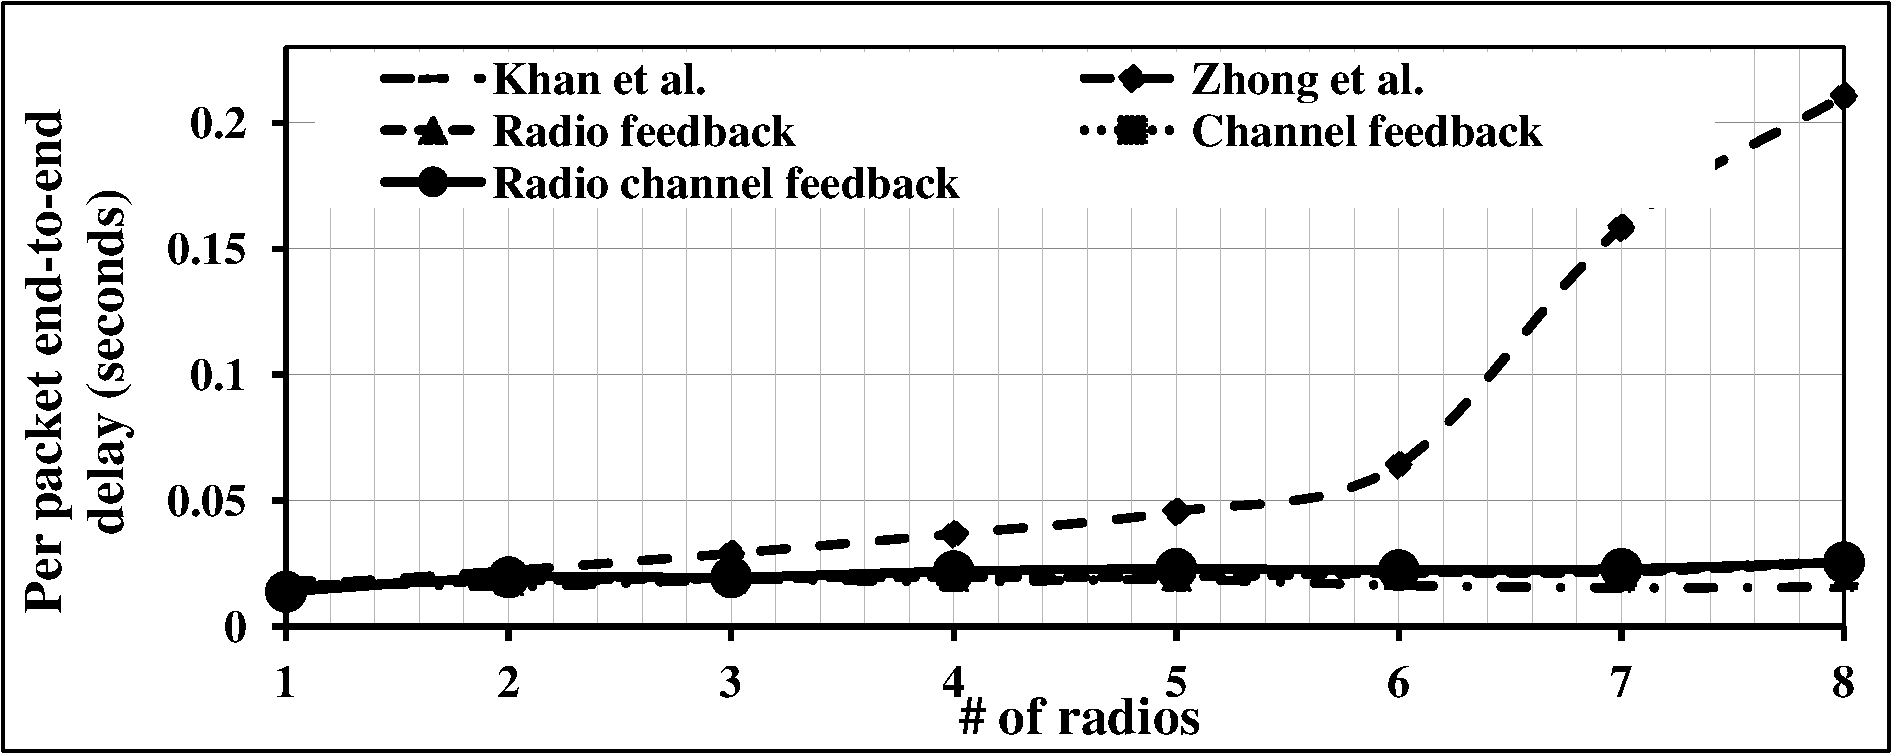
\includegraphics[width=\textwidth]{topology4/Delay24d2}
        \caption{2Mbps application data rate}
        \label{fig:topology4D2}
    \end{subfigure}
    ~\\
    \begin{subfigure}[t]{0.45\textwidth}
        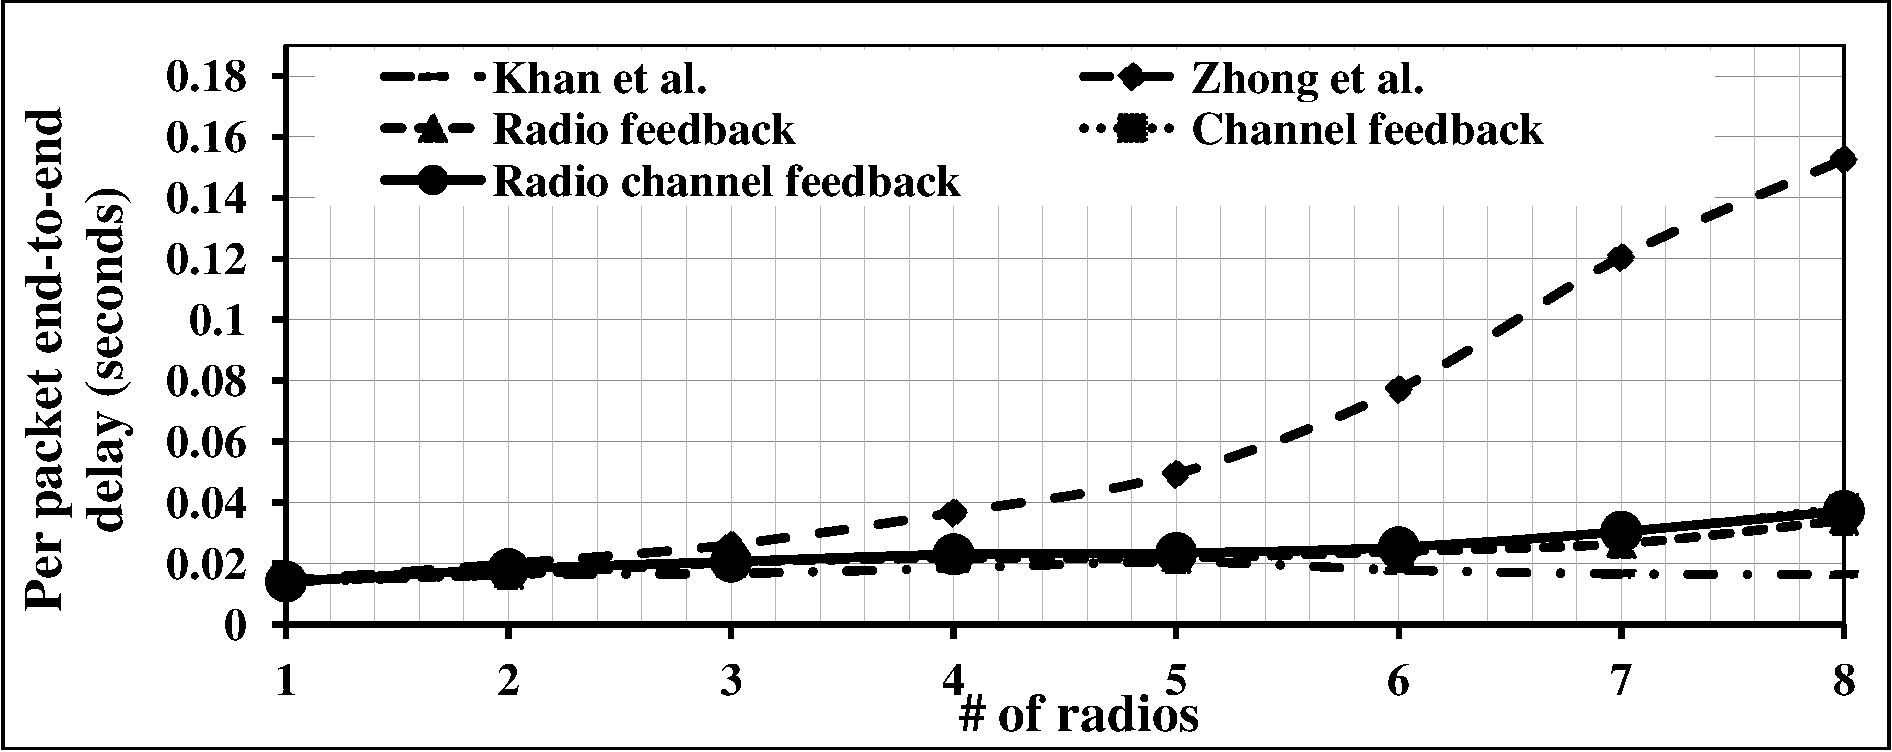
\includegraphics[width=\textwidth]{topology4/Delay24d4}
        \caption{4Mbps application data rate}
        \label{fig:topology4D3}
    \end{subfigure}
    ~
    \begin{subfigure}[t]{0.45\textwidth}
        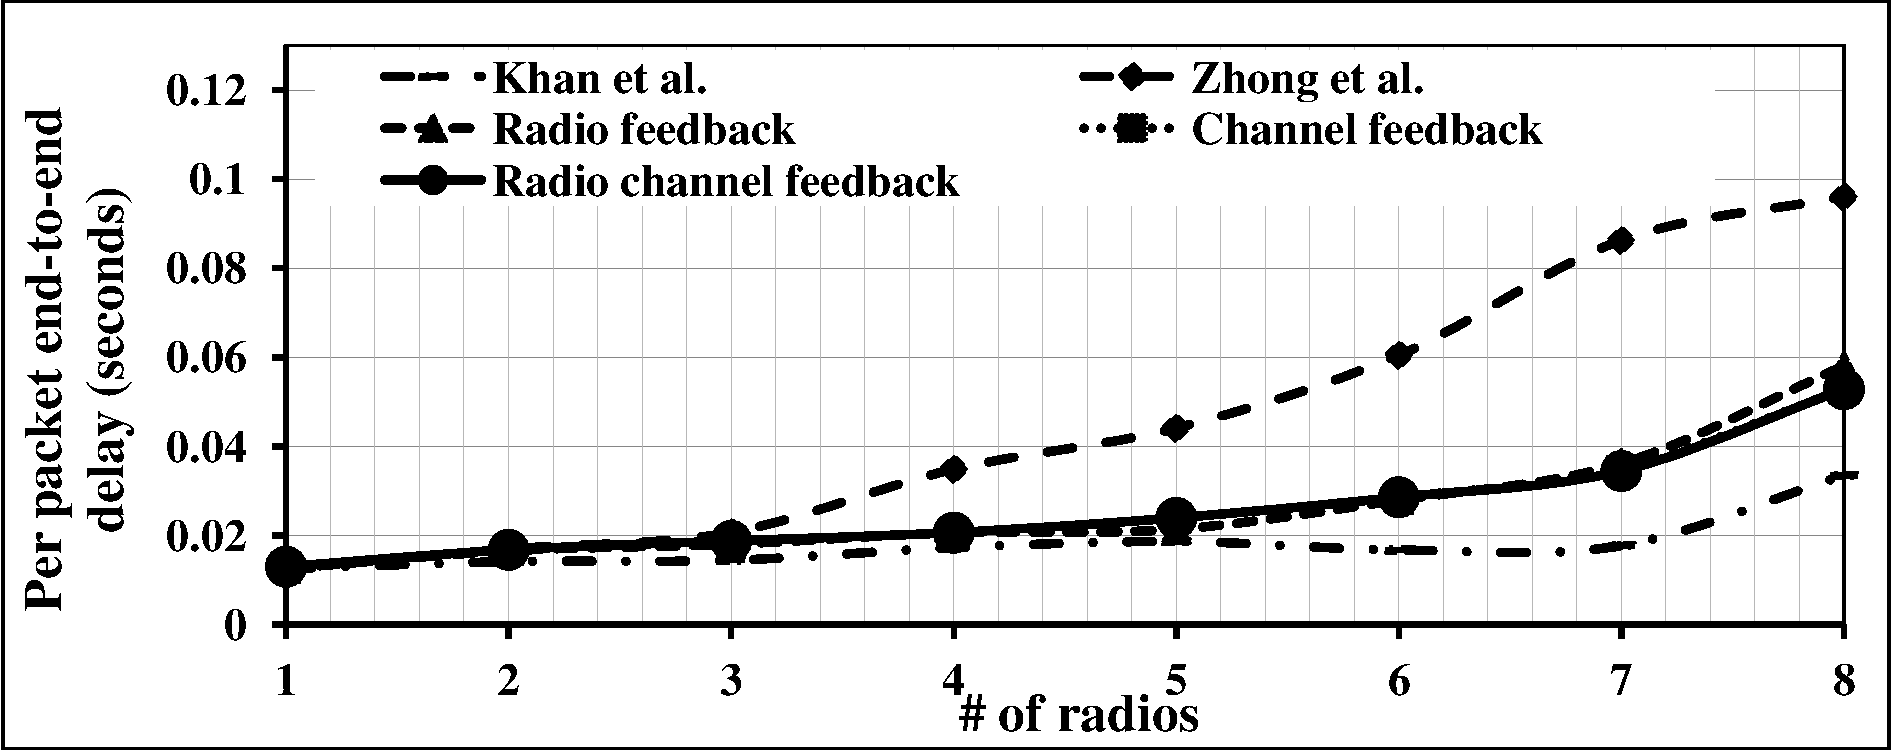
\includegraphics[width=\textwidth]{topology4/Delay24d8}
        \caption{8Mbps application data rate}
        \label{fig:topology4D4}
    \end{subfigure}
    ~\\
    \begin{subfigure}[t]{0.45\textwidth}
        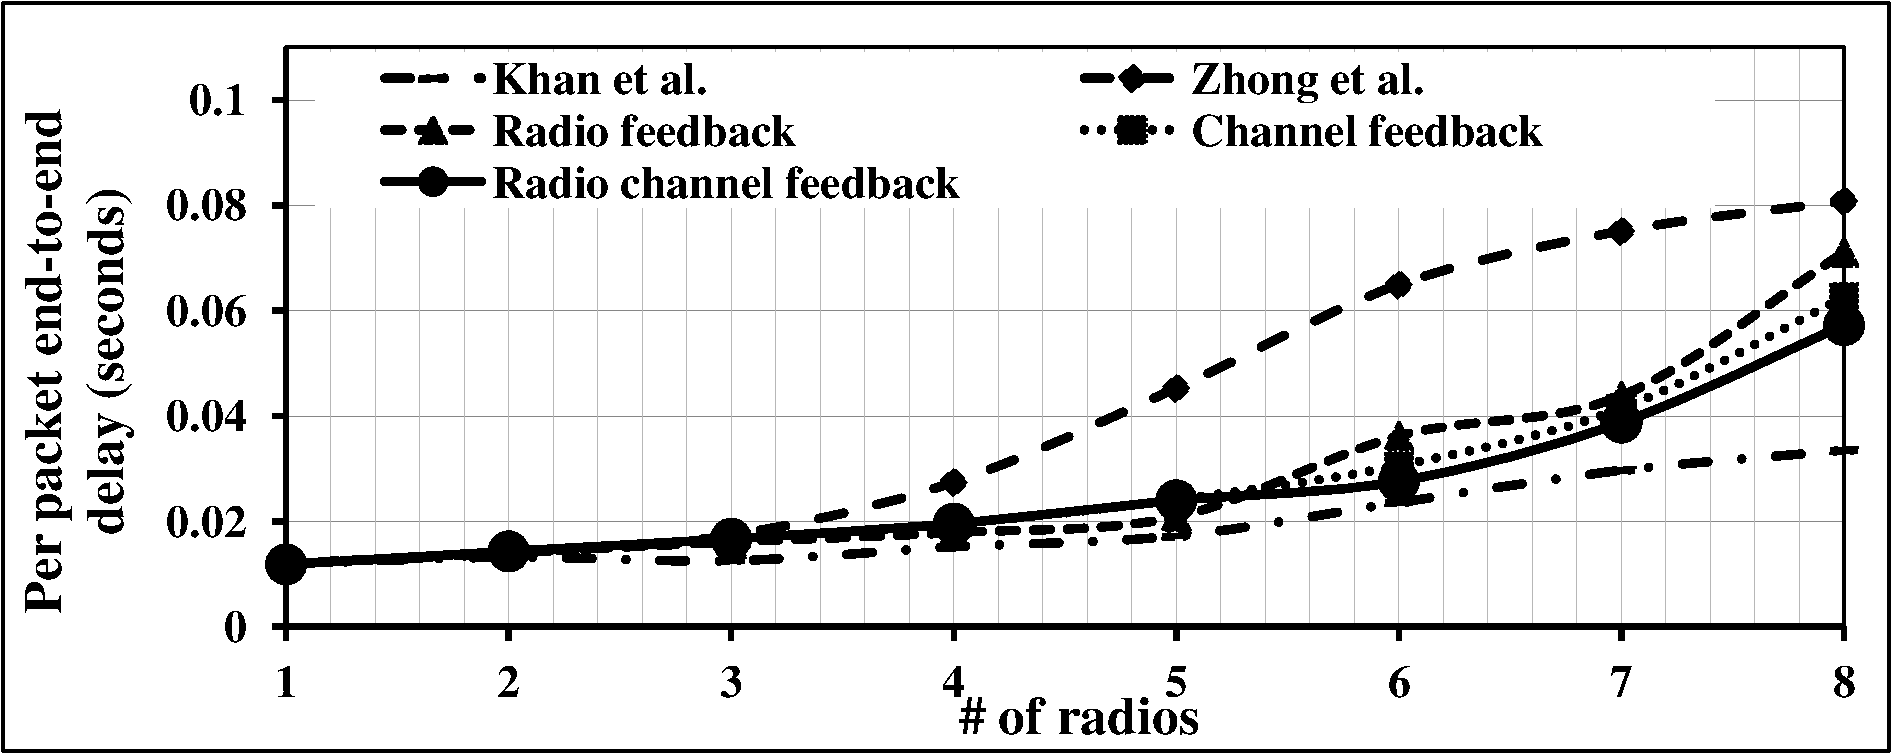
\includegraphics[width=\textwidth]{topology4/Delay24d16}
        \caption{16Mbps application data rate}
        \label{fig:topology4D5}
    \end{subfigure}
    ~
    \begin{subfigure}[t]{0.45\textwidth}
        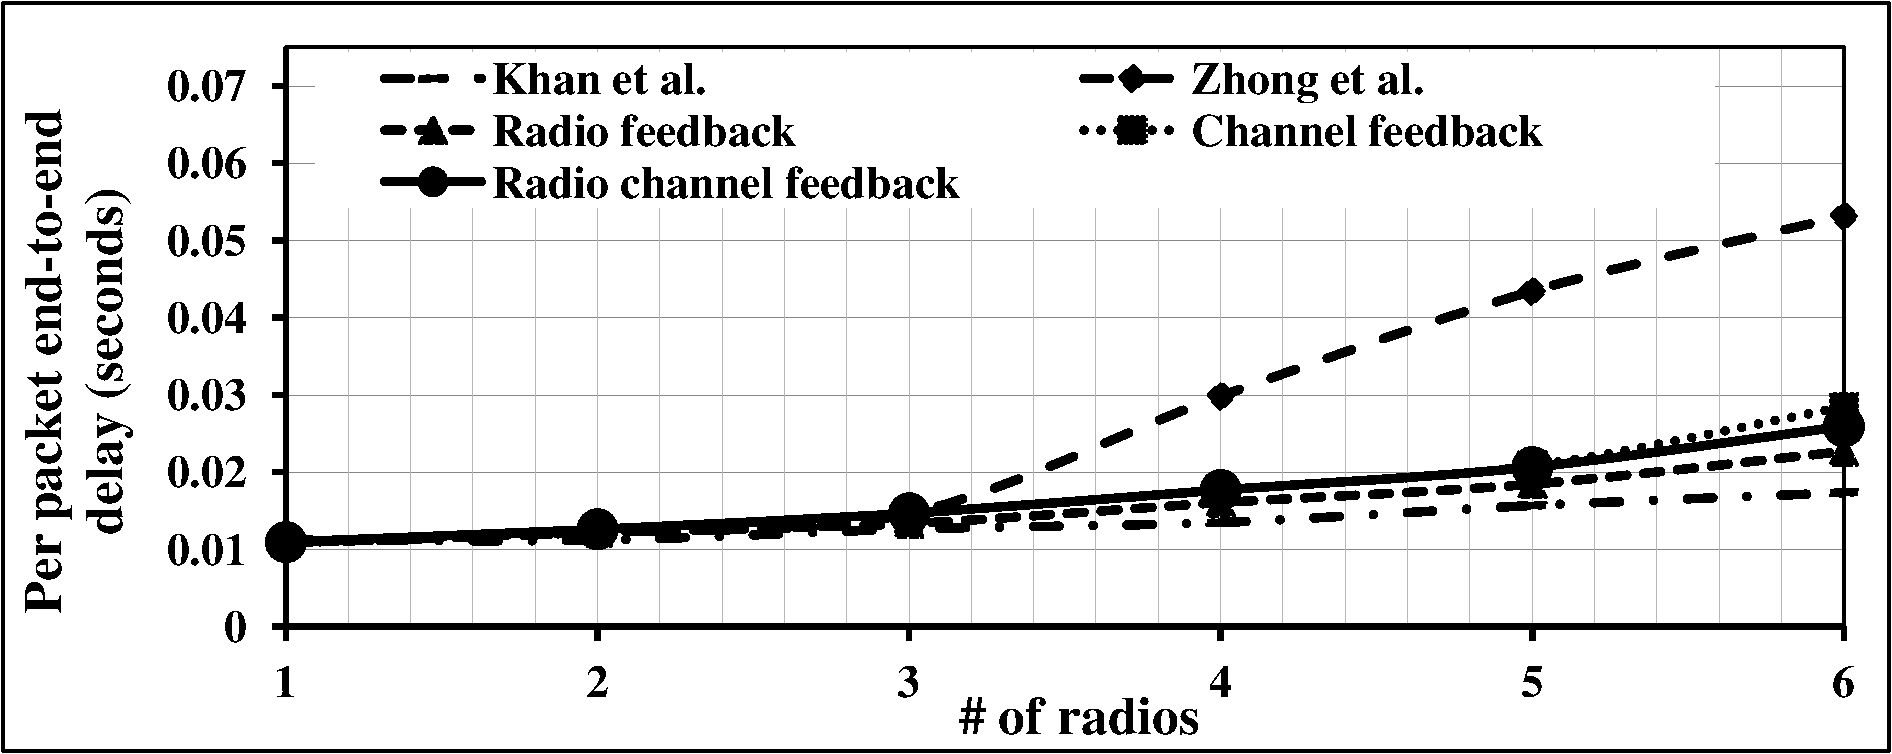
\includegraphics[width=\textwidth]{topology4/Delay24d32}
        \caption{32Mbps application data rate}
        \label{fig:topology4D6}
    \end{subfigure}
    \caption{Average end-to-end delay with varying number of radios for various application data rates}
    \label{fig:topology4D}
\end{figure*}

\begin{landscape}
\begin{figure*}[!htbp]
    \centering
    \begin{subfigure}[t]{0.625\textwidth}
        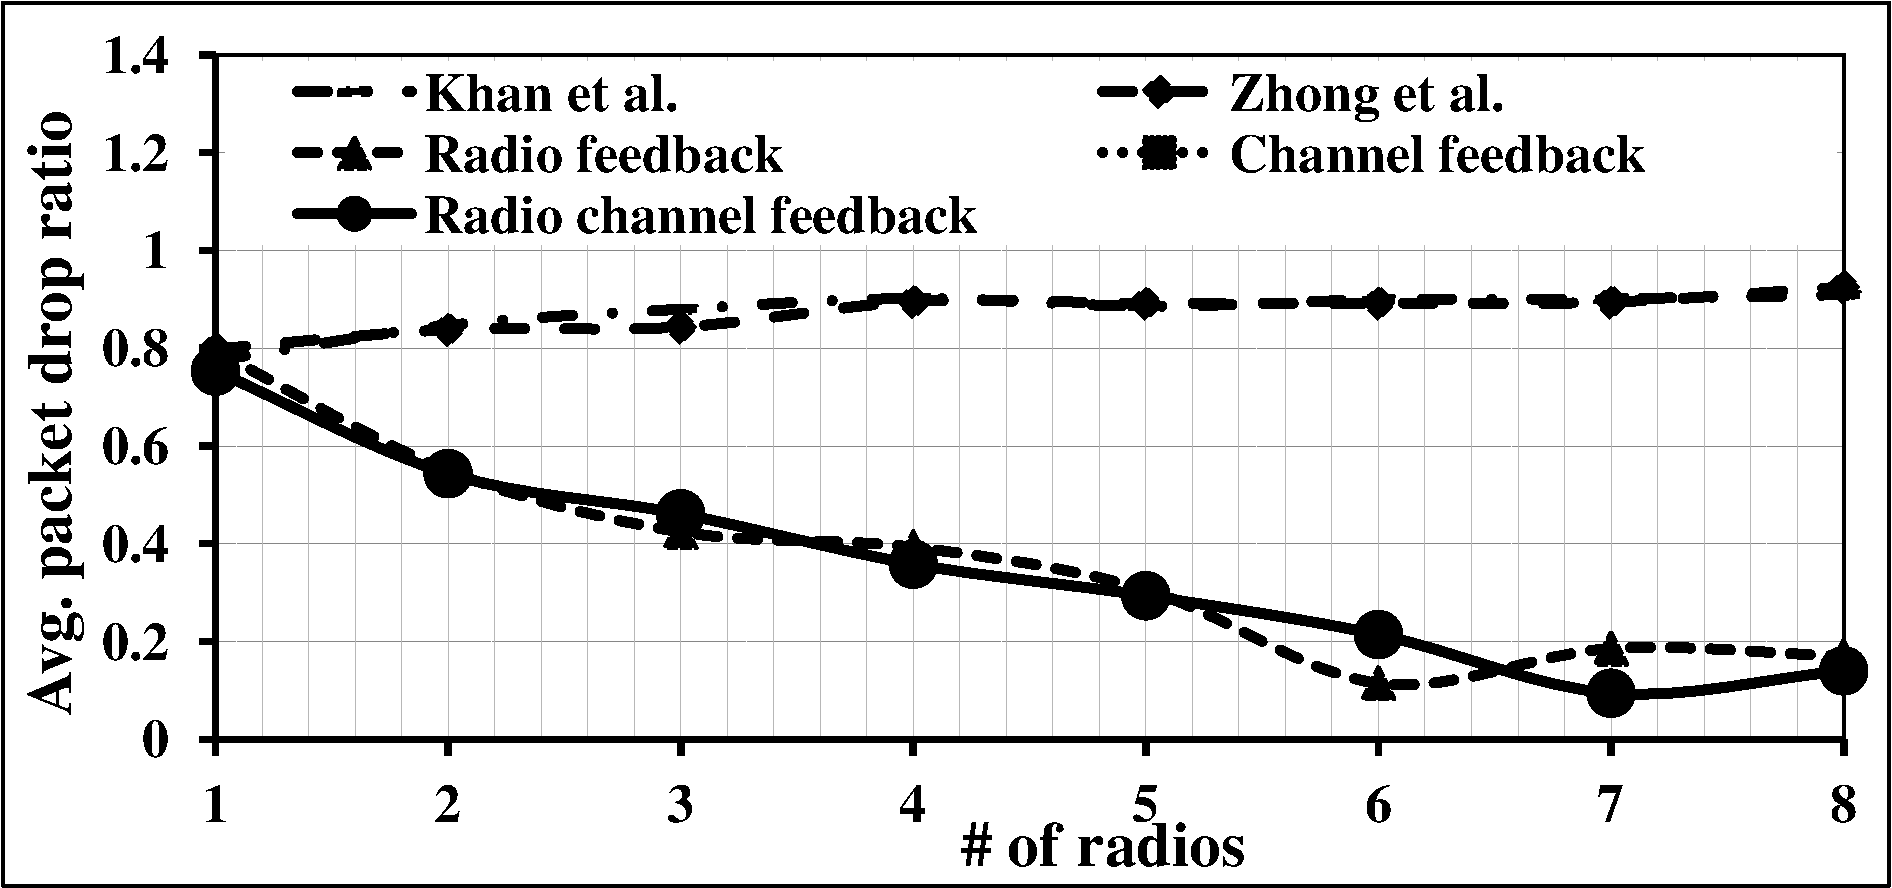
\includegraphics[width=\textwidth]{topology4/PacketDropRatio24d1}
        \caption{1Mbps application data rate}
        \label{fig:topology4P1}
    \end{subfigure}
    ~
    \begin{subfigure}[t]{0.625\textwidth}
        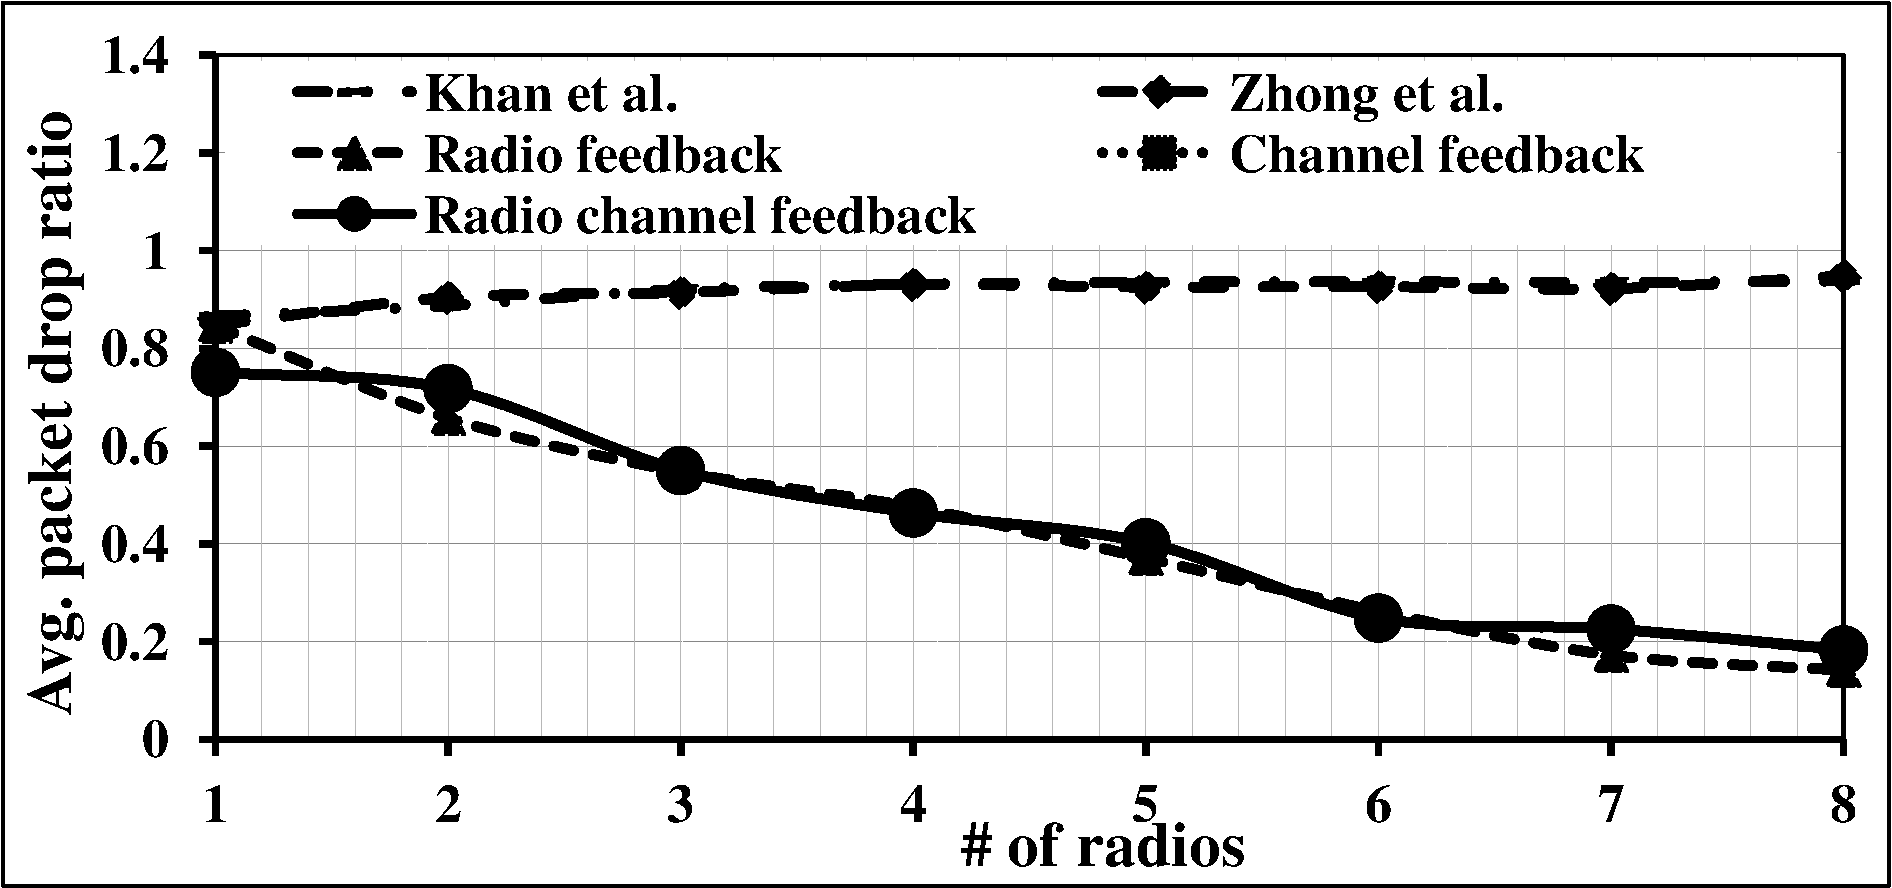
\includegraphics[width=\textwidth]{topology4/PacketDropRatio24d2}
        \caption{2Mbps application data rate}
        \label{fig:topology4P2}
    \end{subfigure}
    ~\\
    \begin{subfigure}[t]{0.625\textwidth}
        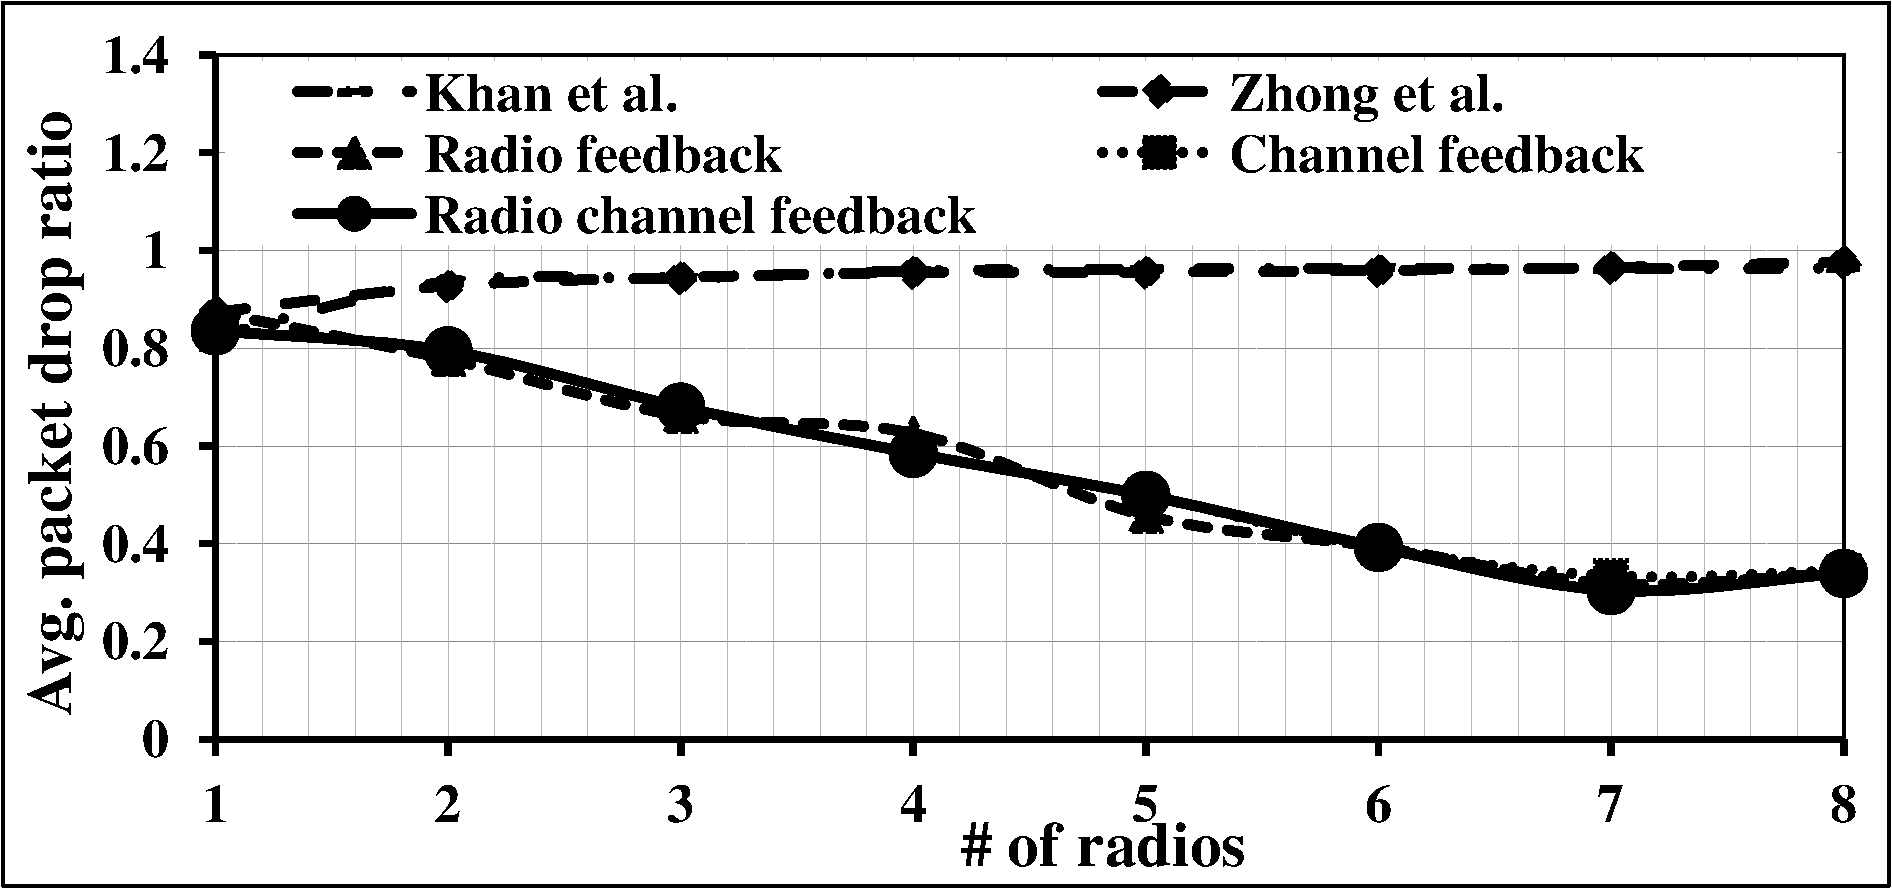
\includegraphics[width=\textwidth]{topology4/PacketDropRatio24d4}
        \caption{4Mbps application data rate}
        \label{fig:topology4P3}
    \end{subfigure}
    ~
    \begin{subfigure}[t]{0.625\textwidth}
        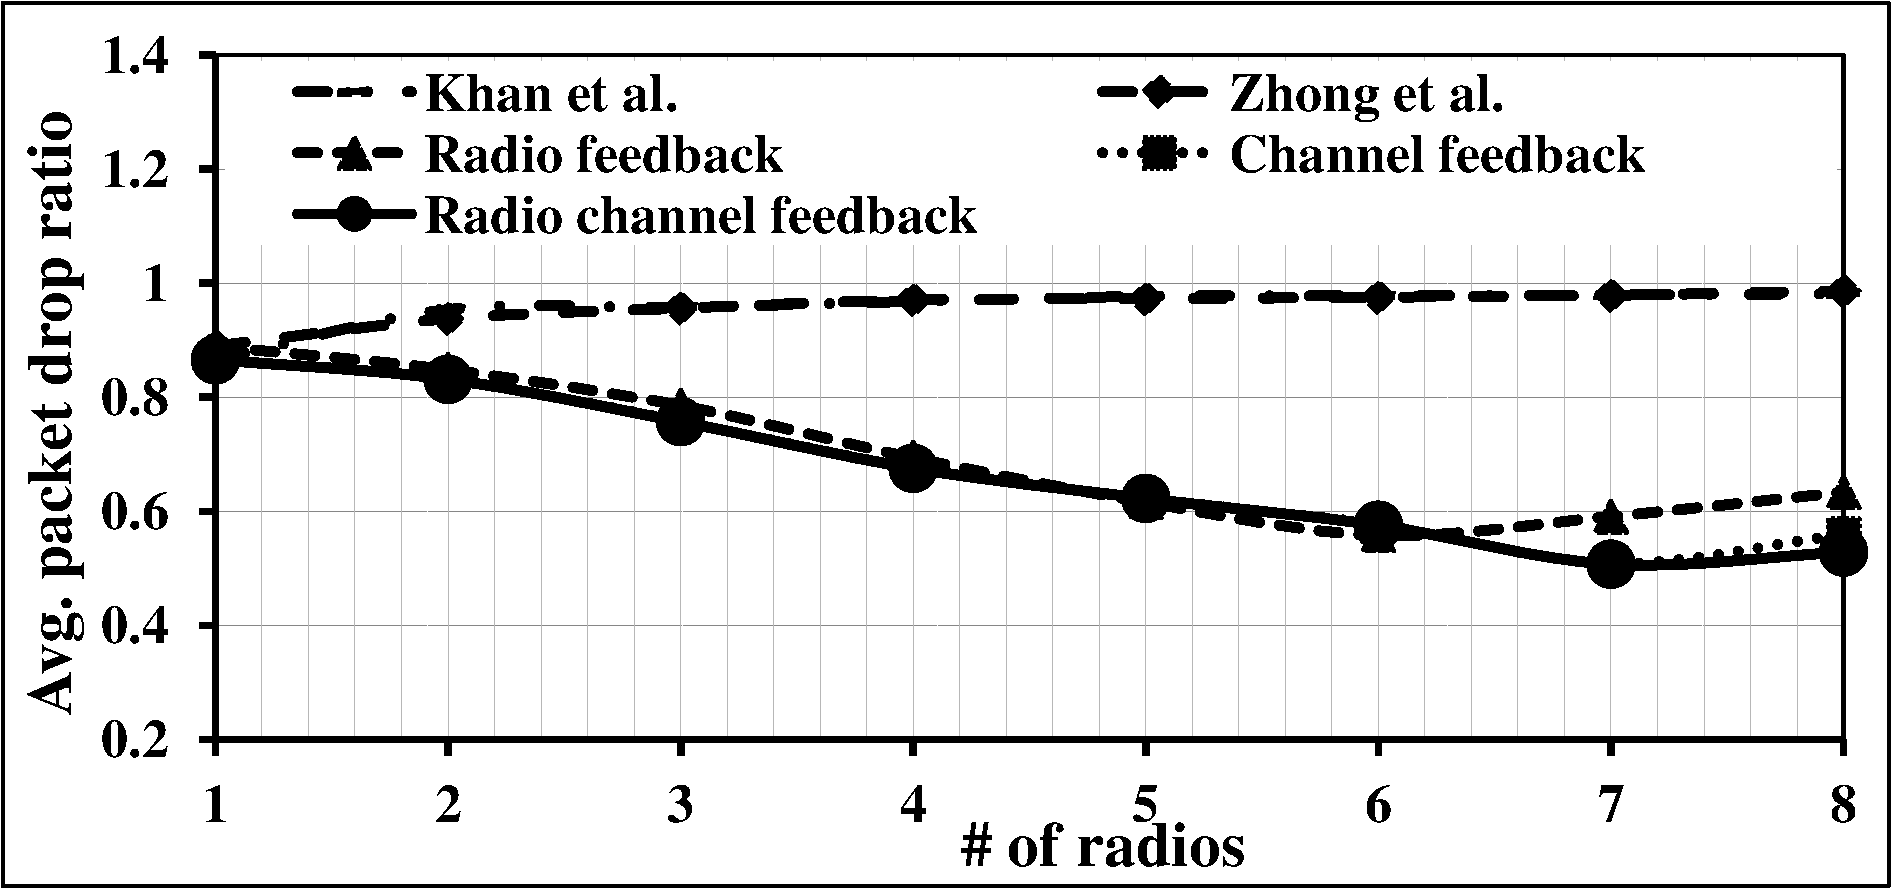
\includegraphics[width=\textwidth]{topology4/PacketDropRatio24d8}
        \caption{8Mbps application data rate}
        \label{fig:topology4P4}
    \end{subfigure}
    ~\\
    \begin{subfigure}[t]{0.625\textwidth}
        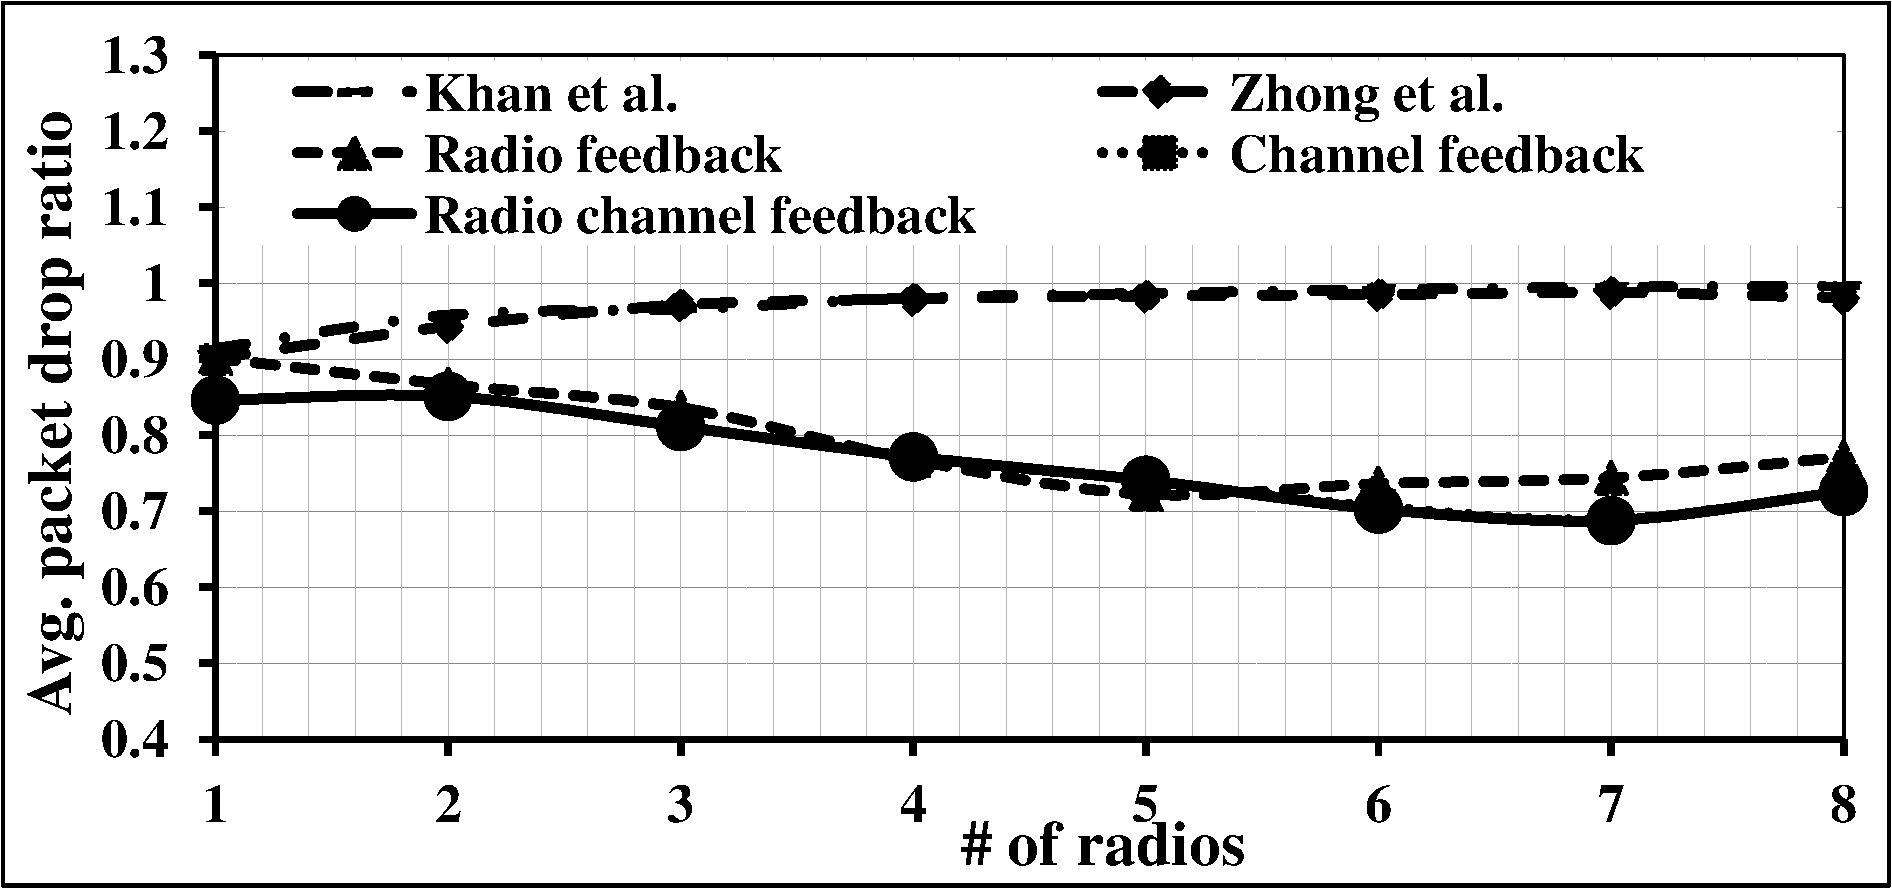
\includegraphics[width=\textwidth]{topology4/PacketDropRatio24d16}
        \caption{16Mbps application data rate}
        \label{fig:topology4P5}
    \end{subfigure}
    ~
    \begin{subfigure}[t]{0.625\textwidth}
        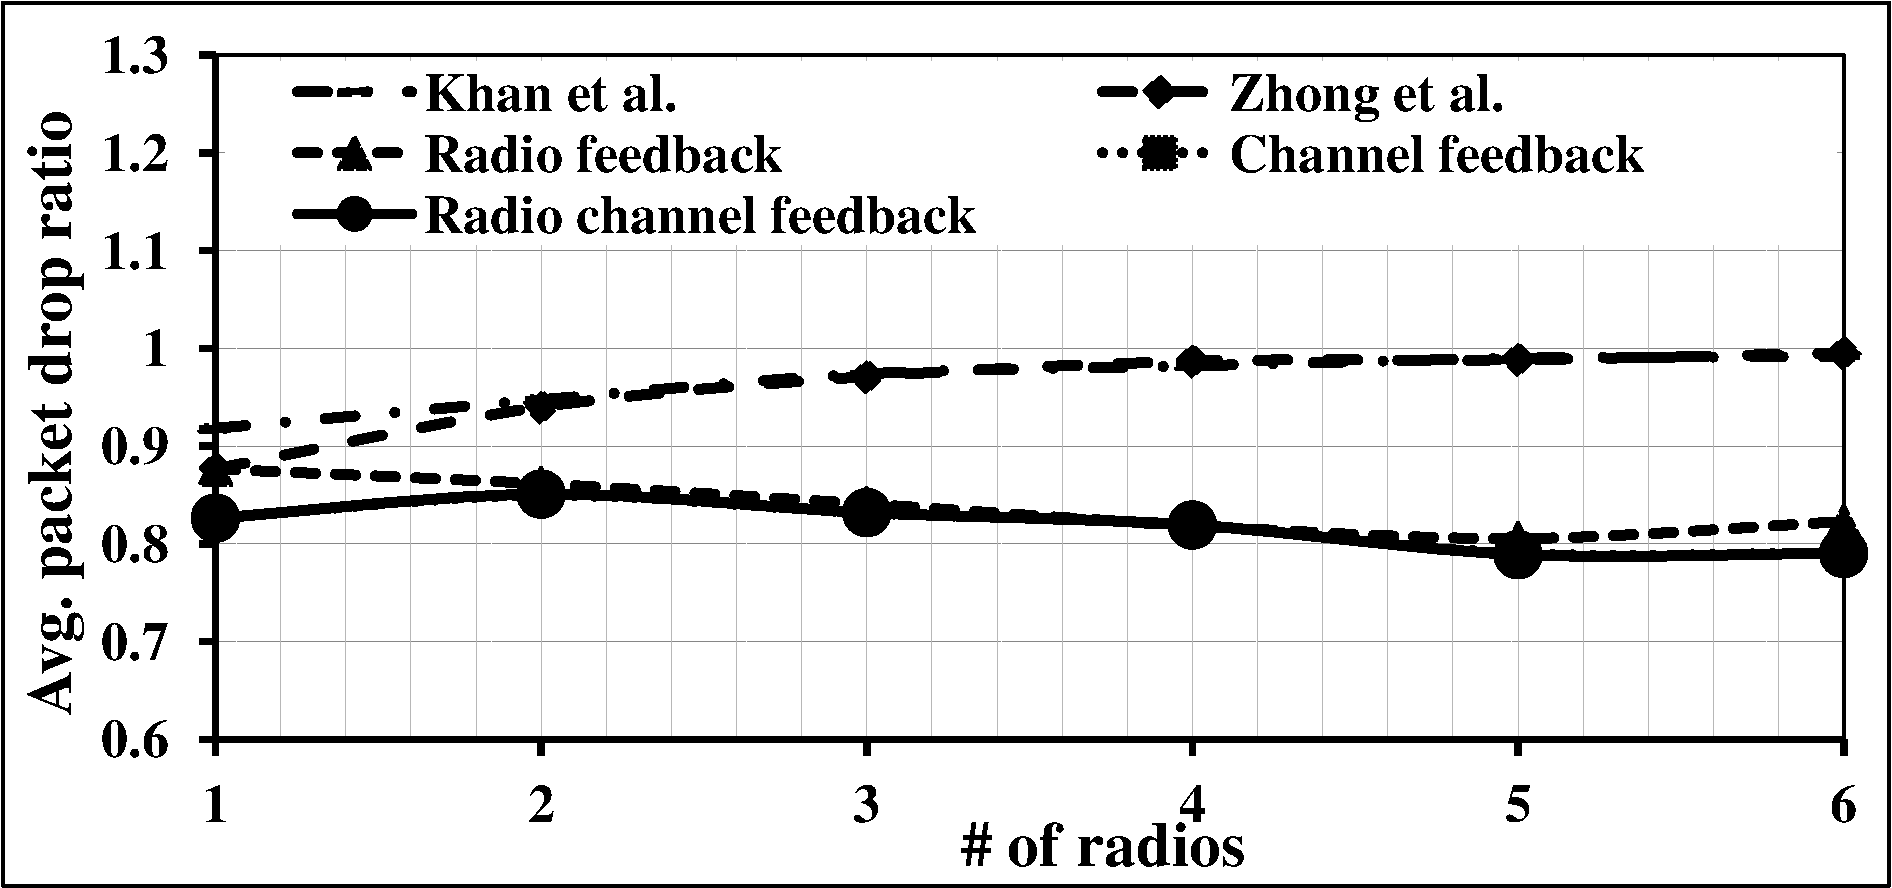
\includegraphics[width=\textwidth]{topology4/PacketDropRatio24d32}
        \caption{32Mbps application data rate}
        \label{fig:topology4P6}
    \end{subfigure}
    \caption{Average packet drop ratio with varying number of radios for various application data rates}
    \label{fig:topology4P}
\end{figure*}
\end{landscape}

\begin{figure*}[!htbp]
    \centering
    \begin{subfigure}[t]{0.45\textwidth}
        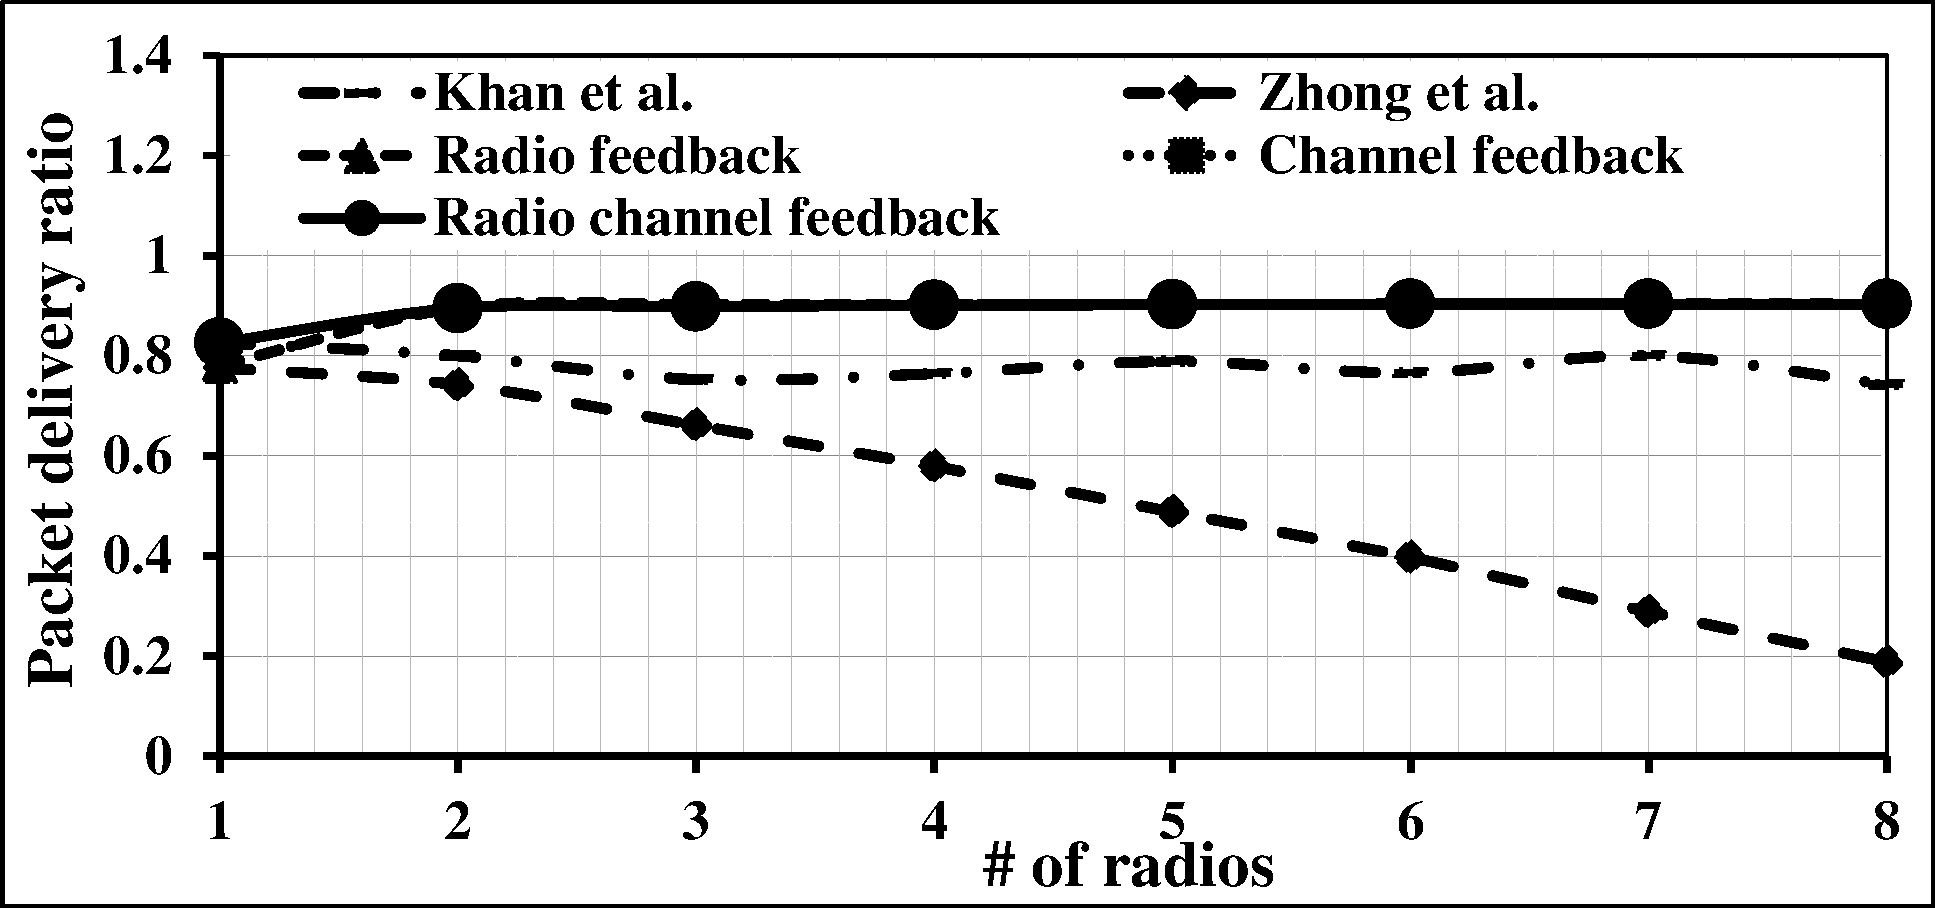
\includegraphics[width=\textwidth]{topology4/DeliveryRatio24d1}
        \caption{1Mbps application data rate}
        \label{fig:topology4PD1}
    \end{subfigure}
    ~
    \begin{subfigure}[t]{0.45\textwidth}
        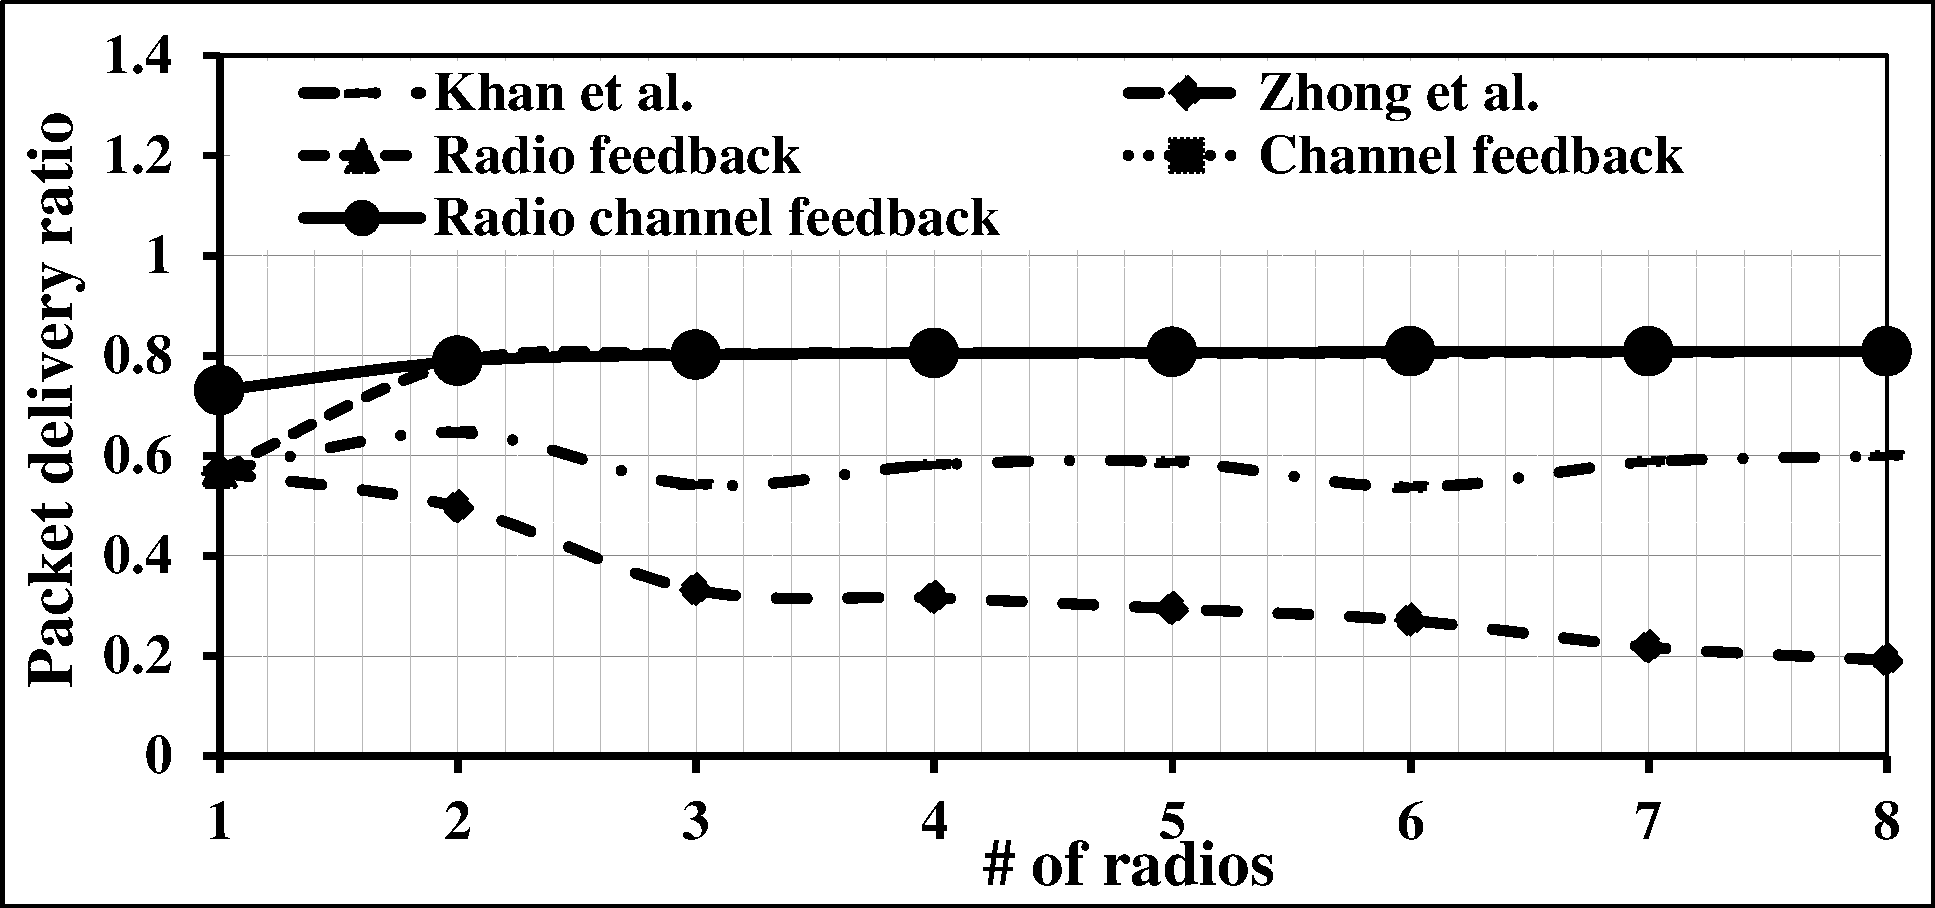
\includegraphics[width=\textwidth]{topology4/DeliveryRatio24d2}
        \caption{2Mbps application data rate}
        \label{fig:topology4PD2}
    \end{subfigure}
    ~\\
    \begin{subfigure}[t]{0.45\textwidth}
        \includegraphics[width=\textwidth]{topology4/DeliveryRatio24d4}
        \caption{4Mbps application data rate}
        \label{fig:topology4PD3}
    \end{subfigure}
    ~
    \begin{subfigure}[t]{0.45\textwidth}
        \includegraphics[width=\textwidth]{topology4/DeliveryRatio24d8}
        \caption{8Mbps application data rate}
        \label{fig:topology4PD4}
    \end{subfigure}
    ~\\
    \begin{subfigure}[t]{0.45\textwidth}
        \includegraphics[width=\textwidth]{topology4/DeliveryRatio24d16}
        \caption{16Mbps application data rate}
        \label{fig:topology4PD5}
    \end{subfigure}
    ~
    \begin{subfigure}[t]{0.45\textwidth}
        \includegraphics[width=\textwidth]{topology4/DeliveryRatio24d32}
        \caption{32Mbps application data rate}
        \label{fig:topology4PD6}
    \end{subfigure}
    \caption{Application layer packet delivery ratio with varying number of radios for various application data rates}
    \label{fig:topology4PD}
\end{figure*}



\begin{table}[!htb]
	\centering
    \caption{Performance improvement achieved using the radio feedback-based approach with respect to the approaches proposed by Khan et al.,~\cite{khan2015towards} and Zhong et al.,~\cite{zhong2014capacity}}
  \label{tab:topology4RadioImprovement}
  \renewcommand\multirowsetup{\centering}
    \begin{tabular}{|>{\centering} p{0.05\textwidth}|c|c|c|c|c|c|c|c|}
    \hline
    \multirow{2}{0.05\textwidth}{\newline \newline \newline Appli-\\cation data rate} & \multicolumn{2}{|p{0.08\textwidth}|}{\centering\% increase in throughput with respect to} & \multicolumn{2}{|p{0.08\textwidth}|}{\centering\% decrease in end-to-end delay with respect to} & \multicolumn{2}{|p{0.08\textwidth}|}{\centering\% decrease in packet drop ratio with respect to} & \multicolumn{2}{|p{0.08\textwidth}|}{\centering\% increase in application layer packet delivery ratio with respect to}\\
    \cline{2-9}
          & \multicolumn{1}{|p{0.025\textwidth}|}{\centering Khan et al.} & \multicolumn{1}{|p{0.025\textwidth}|}{\centering Zhong et al.} & \multicolumn{1}{|p{0.025\textwidth}|}{\centering Khan et al.} & \multicolumn{1}{|p{0.025\textwidth}|}{\centering Zhong et al.} & \multicolumn{1}{|p{0.03\textwidth}|}{\centering Khan et al.} & \multicolumn{1}{|p{0.025\textwidth}|}{\centering Zhong et al.} & \multicolumn{1}{|p{0.025\textwidth}|}{\centering Khan et al.} & \multicolumn{1}{|p{0.025\textwidth}|}{\centering Zhong et al.}\\
    \hline
    1Mbps & 55 & 14 & -9 & 48 & 57 & 57 & 12 & 12 \\\hline
    2Mbps & 64 & 33 & -10 & 50 & 52 & 54 & 24 & 27 \\\hline
    4Mbps & 66 & 44 & -16 & 45 & 40 & 41 & 52 & 52 \\\hline
    8Mbps & 63 & 46 & -17 & 32 & 26 & 26 & 42 & 43 \\\hline
    16Mbps & 62 & 48 & -16 & 24 & 18 & 18 & 40 & 46 \\\hline
    32Mbps & 63 & 42 & -13 & 28 & 13 & 12 & 69 & 73 \\\hline
    \end{tabular}%
\end{table}

\begin{table}[!htb]
	\centering
    \caption{Performance improvement achieved using the channel feedback-based approach with respect to the approaches proposed by Khan et al.,~\cite{khan2015towards} and Zhong et al.,~\cite{zhong2014capacity}}
  \label{tab:topology4ChannelImprovement}
  \renewcommand\multirowsetup{\centering}
    \begin{tabular}{|>{\centering} p{0.05\textwidth}|c|c|c|c|c|c|c|c|}
    \hline
    \multirow{2}{0.05\textwidth}{\newline \newline \newline Appli-\\cation data rate} & \multicolumn{2}{|p{0.08\textwidth}|}{\centering\% increase in throughput with respect to} & \multicolumn{2}{|p{0.08\textwidth}|}{\centering\% decrease in end-to-end delay with respect to} & \multicolumn{2}{|p{0.08\textwidth}|}{\centering\% decrease in packet drop ratio with respect to} & \multicolumn{2}{|p{0.08\textwidth}|}{\centering\% increase in application layer packet delivery ratio with respect to}\\
    \cline{2-9}
          & \multicolumn{1}{|p{0.025\textwidth}|}{\centering Khan et al.} & \multicolumn{1}{|p{0.025\textwidth}|}{\centering Zhong et al.} & \multicolumn{1}{|p{0.025\textwidth}|}{\centering Khan et al.} & \multicolumn{1}{|p{0.025\textwidth}|}{\centering Zhong et al.} & \multicolumn{1}{|p{0.03\textwidth}|}{\centering Khan et al.} & \multicolumn{1}{|p{0.025\textwidth}|}{\centering Zhong et al.} & \multicolumn{1}{|p{0.025\textwidth}|}{\centering Khan et al.} & \multicolumn{1}{|p{0.025\textwidth}|}{\centering Zhong et al.}\\
    \hline
    1Mbps & 55 & 15 & -8 & 49 & 58 & 58 & 12 & 41 \\\hline 
    2Mbps & 63 & 31 & -15 & 48 & 51 & 51 & 27 & 55 \\\hline 
    4Mbps & 66 & 44 & -11 & 42 & 40 & 38 & 52 & 52 \\\hline 
    8Mbps & 64 & 49 & -16 & 31 & 30 & 30 & 44 & 48\\\hline 
    16Mbps & 68 & 55 & -13 & 25 & 21 & 20 & 45 & 47 \\\hline 
    32Mbps & 64 & 44 & -16 & 23 & 15 & 15 & 73 & 68 \\\hline 
    \end{tabular}%
\end{table}

\begin{table}[!htb]
	\centering
    \caption{Performance improvement achieved using the radio channel feedback-based approach with respect to the approaches proposed by Khan et al.,~\cite{khan2015towards} and Zhong et al.,~\cite{zhong2014capacity}}
  \label{tab:topology4RadioChannelImprovement}
  \renewcommand\multirowsetup{\centering}
    \begin{tabular}{|>{\centering} p{0.05\textwidth}|c|c|c|c|c|c|c|c|}
    \hline
    \multirow{2}{0.05\textwidth}{\newline \newline \newline Appli-\\cation data rate} & \multicolumn{2}{|p{0.08\textwidth}|}{\centering\% increase in throughput with respect to} & \multicolumn{2}{|p{0.08\textwidth}|}{\centering\% decrease in end-to-end delay with respect to} & \multicolumn{2}{|p{0.08\textwidth}|}{\centering\% decrease in packet drop ratio with respect to} & \multicolumn{2}{|p{0.08\textwidth}|}{\centering\% increase in application layer packet delivery ratio with respect to}\\
    \cline{2-9}
          & \multicolumn{1}{|p{0.025\textwidth}|}{\centering Khan et al.} & \multicolumn{1}{|p{0.025\textwidth}|}{\centering Zhong et al.} & \multicolumn{1}{|p{0.025\textwidth}|}{\centering Khan et al.} & \multicolumn{1}{|p{0.025\textwidth}|}{\centering Zhong et al.} & \multicolumn{1}{|p{0.03\textwidth}|}{\centering Khan et al.} & \multicolumn{1}{|p{0.025\textwidth}|}{\centering Zhong et al.} & \multicolumn{1}{|p{0.025\textwidth}|}{\centering Khan et al.} & \multicolumn{1}{|p{0.025\textwidth}|}{\centering Zhong et al.}\\
    \hline 
    1Mbps & 55 & 15 & -18 & 49 & 58 & 58 & 42 & 42 \\\hline 
    2Mbps & 63 & 31 & -15 & 49 & 51 & 51 & 58 & 58 \\\hline 
    4Mbps & 66 & 44 & -17 & 42 & 40 & 41 & 57 & 57 \\\hline 
    8Mbps & 63 & 49 & -17 & 31 & 29 & 30 & 49 & 50 \\\hline 
    16Mbps & 68 & 55 & -14 & 27 & 21 & 20 & 53 & 52 \\\hline 
    32Mbps & 64 & 43 & -13 & 23 & 15 & 15 & 73 & 73 \\\hline 
    \end{tabular}%
    \vspace{-0.625cm}
\end{table}


\iffalse
% Table generated by Excel2LaTeX from sheet 'Sheet1'
\begin{table*}[!htbp]
  \centering
  \caption{Percentage improvement achieved using the feedback-based approach with respect to the approaches proposed by Khan et al.,~\cite{khan2015towards} and Zhong et al.,~\cite{zhong2014capacity}}
  \label{tab:topology4Improvement}
    \begin{tabular}{ccccccc}
    \toprule
    \multirow{2}[0]{*}{Application data rate} & \multicolumn{2}{p{0.2\textwidth}}{\% increase in total network througput w.r.t} & \multicolumn{2}{p{0.2\textwidth}}{\% decrease in per packet end-to-end delay w.r.t} & \multicolumn{2}{p{0.2\textwidth}}{\% decrease in packet drop ratio w.r.t} \\
          & \multicolumn{1}{l}{Khan et al.} & \multicolumn{1}{l}{Zhong et al.} & \multicolumn{1}{l}{Khan et al.} & \multicolumn{1}{l}{Zhong et al.} & \multicolumn{1}{l}{Khan et al.} & \multicolumn{1}{l}{Zhong et al.} \\
    \midrule
    1Mbps & 55.862076 & 16.77937765 & -15.155181 & 50.73693391 & 59.865701 & 59.8842253 \\
    2Mbps & 64.74406156 & 33.88792815 & -17.680018 & 51.43200614 & 53.816642 & 53.5899378 \\
    4Mbps & 67.37679147 & 45.85754947 & -30.950717 & 45.37420031 & 41.190572 & 41.8005298 \\
    8Mbps & 65.2701612 & 49.89498939 & -36.956627 & 33.28484049 & 29.774189 & 29.9230113 \\
    16Mbps & 68.48584166 & 55.17376536 & -24.008348 & 28.92168644 & 21.287883 & 20.6884369 \\
    32Mbps & 65.62299103 & 45.56263021 & -13.078491 & 28.3215896 & 15.364822 & 14.5973083 \\
    \bottomrule
    \end{tabular}%
\end{table*}%
\fi


\section{Simulation Findings}

Though we have performed discrete event simulations for various network topologies varying the number of secondary users from 12 to 40 with a granularity of 4, in this thesis, due to space limitation, we have presented the simulation results for only one topology with 24 secondary users. Our proposed approach for CMRNs obtains similar results in case of other seven network topologies as well. Based on these simulation results we obtain following findings:

\begin{itemize}
    \item Over all these topologies, our proposed feedback-based approach improves total network throughput 51\% on an average against that of existing approaches.
    \item Over all these topologies, our proposed feedback-based approach decreases packet drop ratio up to 35\% on an average against that of existing approaches.
    \item Among three variants of our proposed feedback-based approach, radio channel feedback approach marginally (3\%) performs better over other variants.
    \item For CMRNs, our proposed feedback-based approach increases throughput with an increase in number of radios for low to medium (1-8Mbps) data rates. For high data rates (16-32 Mbps), multiple radio introduction could not make significant impact on throughput and throughput usually degrades with an increase in number of radios.
    \item For CMRNs, our proposed feedback-based approach is able to make average end-to-end delay constant with an increase in number of radios for low to medium (1-8Mbps) data rates. For high data rates (16-32 Mbps), delay usually increases with an increase in number of radios.
    \item For CMRNs, our proposed feedback-based approach improves average packet drop ratio with an increase in number of radios for low to medium (1-16Mbps) data rates. For high data rate (32 Mbps), packet drop ratio remains constant with an increase in number of radios.
\end{itemize}

\endinput


%\chapter{Future Work}
We tried our best to perform extensive simulations to validate our proposed approach. However, we are aware of the limitations of simulation. At this time, we do not have any access to a real CR testbed. In future, we plan to validate our presented simulation model with CR testbed. We also plan to formulate analytical models in future. We will model the successful packet transmission probability and PU-free channel selection probability. From these two models, we will formulate the delay and throughput for the proposed MRCRNs architecture. Our proposed approach exploits multiple radios traversing multiple channels at the same time. However, multi-path communication via multiple cognitive radios would be another interesting field to study. In future, we would investigate the performance of MRCRNs exploiting multi-path communication.
\endinput


\chapter{Conclusion}
Cognitive radio networks suffer noteworthy throughput degradation with the introduction of multi-radio usage. We propose a feedback-based multi-radio exploitation approach for CRNs in this paper to overcome this throughput degradation. We implement the proposed approach in ns-3 to measure various performance metrics such as throughput, delay, packet delivery, and drop ratio over numerous network settings. Simulation results reveal that our proposed approach can significantly increase total network throughput and decrease packet drop ratio compared to other existing techniques. Furthermore, the feedback-based approach can be used to find the number of radios needed to experience a delicate tradeoff between network throughput and delay for applications maintaining different data rates. In future, we plan to formulate analytical models of our proposed approach and implement the approach in real testbed.
\endinput


\begin{landscape}
\appendix
\begin{landscape}
\begin{figure*}[!htbp]
    \centering
    \begin{subfigure}[t]{0.625\textwidth}
        \includegraphics[width=\textwidth]{alltopology/12Throughput24d1}
        \caption{1Mbps application data rate}
        \label{fig:alltopologyT1}
    \end{subfigure}
    ~
    \begin{subfigure}[t]{0.625\textwidth}
        \includegraphics[width=\textwidth]{alltopology/12Throughput24d2}
        \caption{2Mbps application data rate}
        \label{fig:alltopologyT2}
    \end{subfigure}
    ~\\
    \begin{subfigure}[t]{0.625\textwidth}
        \includegraphics[width=\textwidth]{alltopology/12Throughput24d4}
        \caption{4Mbps application data rate}
        \label{fig:alltopologyT3}
    \end{subfigure}
    ~
    \begin{subfigure}[t]{0.625\textwidth}
        \includegraphics[width=\textwidth]{alltopology/12Throughput24d8}
        \caption{8Mbps application data rate}
        \label{fig:alltopologyT4}
    \end{subfigure}
    ~\\
    \begin{subfigure}[t]{0.625\textwidth}
        \includegraphics[width=\textwidth]{alltopology/12Throughput24d16}
        \caption{16Mbps application data rate}
        \label{fig:alltopologyT5}
    \end{subfigure}
    ~
    \begin{subfigure}[t]{0.625\textwidth}
        \includegraphics[width=\textwidth]{alltopology/12Throughput24d32}
        \caption{32Mbps application data rate}
        \label{fig:alltopologyT6}
    \end{subfigure}
    \caption{Average network throughput with varying number of radios for various application data rates}
    \label{fig:alltopologyT}
\end{figure*}
\end{landscape}
\end{landscape}
\endinput

\bibliographystyle{unsrt}
%\bibliographystyle{ieeetr}
\bibliography{SystemModel}


\end{document}
